\documentclass[twoside]{book}

% Packages required by doxygen
\usepackage{fixltx2e}
\usepackage{calc}
\usepackage{doxygen}
\usepackage[export]{adjustbox} % also loads graphicx
\usepackage{graphicx}
\usepackage[utf8]{inputenc}
\usepackage{makeidx}
\usepackage{multicol}
\usepackage{multirow}
\PassOptionsToPackage{warn}{textcomp}
\usepackage{textcomp}
\usepackage[nointegrals]{wasysym}
\usepackage[table]{xcolor}

% Font selection
\usepackage[T1]{fontenc}
\usepackage[scaled=.90]{helvet}
\usepackage{courier}
\usepackage{amssymb}
\usepackage{sectsty}
\renewcommand{\familydefault}{\sfdefault}
\allsectionsfont{%
  \fontseries{bc}\selectfont%
  \color{darkgray}%
}
\renewcommand{\DoxyLabelFont}{%
  \fontseries{bc}\selectfont%
  \color{darkgray}%
}
\newcommand{\+}{\discretionary{\mbox{\scriptsize$\hookleftarrow$}}{}{}}

% Page & text layout
\usepackage{geometry}
\geometry{%
  a4paper,%
  top=2.5cm,%
  bottom=2.5cm,%
  left=2.5cm,%
  right=2.5cm%
}
\tolerance=750
\hfuzz=15pt
\hbadness=750
\setlength{\emergencystretch}{15pt}
\setlength{\parindent}{0cm}
\setlength{\parskip}{0.2cm}
\makeatletter
\renewcommand{\paragraph}{%
  \@startsection{paragraph}{4}{0ex}{-1.0ex}{1.0ex}{%
    \normalfont\normalsize\bfseries\SS@parafont%
  }%
}
\renewcommand{\subparagraph}{%
  \@startsection{subparagraph}{5}{0ex}{-1.0ex}{1.0ex}{%
    \normalfont\normalsize\bfseries\SS@subparafont%
  }%
}
\makeatother

% Headers & footers
\usepackage{fancyhdr}
\pagestyle{fancyplain}
\fancyhead[LE]{\fancyplain{}{\bfseries\thepage}}
\fancyhead[CE]{\fancyplain{}{}}
\fancyhead[RE]{\fancyplain{}{\bfseries\leftmark}}
\fancyhead[LO]{\fancyplain{}{\bfseries\rightmark}}
\fancyhead[CO]{\fancyplain{}{}}
\fancyhead[RO]{\fancyplain{}{\bfseries\thepage}}
\fancyfoot[LE]{\fancyplain{}{}}
\fancyfoot[CE]{\fancyplain{}{}}
\fancyfoot[RE]{\fancyplain{}{\bfseries\scriptsize Generated on Wed Jul 11 2018 09\+:37\+:24 for F\+L\+T\+\_\+\+H\+A\+Z by Doxygen }}
\fancyfoot[LO]{\fancyplain{}{\bfseries\scriptsize Generated on Wed Jul 11 2018 09\+:37\+:24 for F\+L\+T\+\_\+\+H\+A\+Z by Doxygen }}
\fancyfoot[CO]{\fancyplain{}{}}
\fancyfoot[RO]{\fancyplain{}{}}
\renewcommand{\footrulewidth}{0.4pt}
\renewcommand{\chaptermark}[1]{%
  \markboth{#1}{}%
}
\renewcommand{\sectionmark}[1]{%
  \markright{\thesection\ #1}%
}

% Indices & bibliography
\usepackage{natbib}
\usepackage[titles]{tocloft}
\setcounter{tocdepth}{3}
\setcounter{secnumdepth}{5}
\makeindex

% Hyperlinks (required, but should be loaded last)
\usepackage{ifpdf}
\ifpdf
  \usepackage[pdftex,pagebackref=true]{hyperref}
\else
  \usepackage[ps2pdf,pagebackref=true]{hyperref}
\fi
\hypersetup{%
  colorlinks=true,%
  linkcolor=blue,%
  citecolor=blue,%
  unicode%
}

% Custom commands
\newcommand{\clearemptydoublepage}{%
  \newpage{\pagestyle{empty}\cleardoublepage}%
}


%===== C O N T E N T S =====

\begin{document}

% Titlepage & ToC
\hypersetup{pageanchor=false,
             bookmarks=true,
             bookmarksnumbered=true,
             pdfencoding=unicode
            }
\pagenumbering{roman}
\begin{titlepage}
\vspace*{7cm}
\begin{center}%
{\Large F\+L\+T\+\_\+\+H\+A\+Z }\\
\vspace*{1cm}
{\large Generated by Doxygen 1.8.10}\\
\vspace*{0.5cm}
{\small Wed Jul 11 2018 09:37:24}\\
\end{center}
\end{titlepage}
\clearemptydoublepage
\tableofcontents
\clearemptydoublepage
\pagenumbering{arabic}
\hypersetup{pageanchor=true}

%--- Begin generated contents ---
\chapter{Modules Index}
\section{Modules List}
Here is a list of all modules with brief descriptions\+:\begin{DoxyCompactList}
\item\contentsline{section}{\hyperlink{namespaceconst__module}{const\+\_\+module} }{\pageref{namespaceconst__module}}{}
\item\contentsline{section}{\hyperlink{namespaceflt__module}{flt\+\_\+module} }{\pageref{namespaceflt__module}}{}
\item\contentsline{section}{\hyperlink{namespacegmpe__module}{gmpe\+\_\+module} }{\pageref{namespacegmpe__module}}{}
\item\contentsline{section}{\hyperlink{namespaceinput__module}{input\+\_\+module} }{\pageref{namespaceinput__module}}{}
\item\contentsline{section}{\hyperlink{namespaceutils}{utils} }{\pageref{namespaceutils}}{}
\end{DoxyCompactList}

\chapter{File Index}
\section{File List}
Here is a list of all files with brief descriptions\+:\begin{DoxyCompactList}
\item\contentsline{section}{\hyperlink{const__module_8f90}{const\+\_\+module.\+f90} }{\pageref{const__module_8f90}}{}
\item\contentsline{section}{\hyperlink{flt__module_8f90}{flt\+\_\+module.\+f90} }{\pageref{flt__module_8f90}}{}
\item\contentsline{section}{\hyperlink{_g_m_p_e__module_8f90}{G\+M\+P\+E\+\_\+module.\+f90} }{\pageref{_g_m_p_e__module_8f90}}{}
\item\contentsline{section}{\hyperlink{input__module_8f90}{input\+\_\+module.\+f90} }{\pageref{input__module_8f90}}{}
\item\contentsline{section}{\hyperlink{main__flt__haz_8f90}{main\+\_\+flt\+\_\+haz.\+f90} }{\pageref{main__flt__haz_8f90}}{}
\item\contentsline{section}{\hyperlink{utils_8f90}{utils.\+f90} }{\pageref{utils_8f90}}{}
\end{DoxyCompactList}

\chapter{Module Documentation}
\hypertarget{namespaceconst__module}{}\section{const\+\_\+module Module Reference}
\label{namespaceconst__module}\index{const\+\_\+module@{const\+\_\+module}}
\subsection*{Variables}
\begin{DoxyCompactItemize}
\item 
real(8), parameter \hyperlink{namespaceconst__module_a6e2d7a0e80dfe577ca95736d3e143899}{pi} = 3.\+14159265358979
\item 
real(8), parameter \hyperlink{namespaceconst__module_a87cf12ab3afb0ddc5f58492d1fb1d828}{deg2rad} = 0.\+0174532925199433
\item 
real(8), parameter \hyperlink{namespaceconst__module_a61843a48c8dec76293f423c682c8d772}{rad2deg} = 57.\+2957795130823
\item 
real(8), parameter \hyperlink{namespaceconst__module_aa70be203aa6a91ce3961b81a6eae1e60}{sqrt2\+\_\+inv} = 0.\+707106781186547
\item 
real(8), parameter \hyperlink{namespaceconst__module_ab766035166a55b031df25669f66e7b06}{earth\+\_\+r} = 6371.\+0
\item 
integer, parameter \hyperlink{namespaceconst__module_afdf6c6b7ffea232bbc86b7ffef8298dc}{ss} = 1
\item 
integer, parameter \hyperlink{namespaceconst__module_a2fac1c74f2a81234dec392f6ad1c73ea}{rv} = 2
\item 
integer, parameter \hyperlink{namespaceconst__module_a45c7ab4515e2c0068ca69e5f4fed8a51}{nm} = 3
\item 
integer, parameter \hyperlink{namespaceconst__module_a437f551584bfdf420d4b28c829759eb5}{na} = 4
\item 
integer, parameter \hyperlink{namespaceconst__module_a760935a100ba2e8695aa777f582d5a61}{wc94} = 1
\item 
integer, parameter \hyperlink{namespaceconst__module_a28954bb32bf9368bbb5569a257603c57}{peer} = 2
\item 
integer, parameter \hyperlink{namespaceconst__module_a6d9b6ff754fe58527edcaea132c3d736}{ceus} = 3
\item 
integer, parameter \hyperlink{namespaceconst__module_aac415d96f710c33f0228284d6f5504c9}{point} = 4
\item 
integer, parameter \hyperlink{namespaceconst__module_a7b2347a542b2eda2b6841e1d9fdf19f4}{exponential} = 1
\item 
integer, parameter \hyperlink{namespaceconst__module_ab9dc6742ce1e2309dd194ecdd254779d}{characteristic} = 2
\item 
integer, parameter \hyperlink{namespaceconst__module_a6bed9e9fc42a9b205a9214865ad145f5}{delta} = 3
\item 
integer, parameter \hyperlink{namespaceconst__module_ad7dece49d5a2db833c491ea2eed54f52}{deg} = 1
\item 
integer, parameter \hyperlink{namespaceconst__module_a4e8504d7945ca96447c578c95644bd5a}{km} = 2
\item 
integer, parameter \hyperlink{namespaceconst__module_a83696a36c5a2e83e44cbfbbc479717a9}{sadigh97} = 1
\item 
integer, parameter \hyperlink{namespaceconst__module_ac32c40069d129a7d06c22292afaae3ba}{cy14} = 2
\item 
integer, parameter \hyperlink{namespaceconst__module_a91a738fc17a72ffc4e34e5141cccc469}{uniform} = 1
\item 
integer, parameter \hyperlink{namespaceconst__module_a7e2946932c4a8471477923bc49aeafe4}{triangular} = 2
\item 
integer, parameter \hyperlink{namespaceconst__module_a8010dcce5207fede7f1da8dbde0b5be8}{normal} = 1
\item 
integer, parameter \hyperlink{namespaceconst__module_a3895bfacad51cb8237e9cae087b1663a}{trunc\+\_\+normal} = 2
\item 
integer, parameter \hyperlink{namespaceconst__module_a0a0ee9e64316ae52e9c539987c5d18d5}{heaviside} = 3
\end{DoxyCompactItemize}


\subsection{Variable Documentation}
\hypertarget{namespaceconst__module_a6d9b6ff754fe58527edcaea132c3d736}{}\index{const\+\_\+module@{const\+\_\+module}!ceus@{ceus}}
\index{ceus@{ceus}!const\+\_\+module@{const\+\_\+module}}
\subsubsection[{ceus}]{\setlength{\rightskip}{0pt plus 5cm}integer, parameter const\+\_\+module\+::ceus = 3}\label{namespaceconst__module_a6d9b6ff754fe58527edcaea132c3d736}
\hypertarget{namespaceconst__module_ab9dc6742ce1e2309dd194ecdd254779d}{}\index{const\+\_\+module@{const\+\_\+module}!characteristic@{characteristic}}
\index{characteristic@{characteristic}!const\+\_\+module@{const\+\_\+module}}
\subsubsection[{characteristic}]{\setlength{\rightskip}{0pt plus 5cm}integer, parameter const\+\_\+module\+::characteristic = 2}\label{namespaceconst__module_ab9dc6742ce1e2309dd194ecdd254779d}
\hypertarget{namespaceconst__module_ac32c40069d129a7d06c22292afaae3ba}{}\index{const\+\_\+module@{const\+\_\+module}!cy14@{cy14}}
\index{cy14@{cy14}!const\+\_\+module@{const\+\_\+module}}
\subsubsection[{cy14}]{\setlength{\rightskip}{0pt plus 5cm}integer, parameter const\+\_\+module\+::cy14 = 2}\label{namespaceconst__module_ac32c40069d129a7d06c22292afaae3ba}
\hypertarget{namespaceconst__module_ad7dece49d5a2db833c491ea2eed54f52}{}\index{const\+\_\+module@{const\+\_\+module}!deg@{deg}}
\index{deg@{deg}!const\+\_\+module@{const\+\_\+module}}
\subsubsection[{deg}]{\setlength{\rightskip}{0pt plus 5cm}integer, parameter const\+\_\+module\+::deg = 1}\label{namespaceconst__module_ad7dece49d5a2db833c491ea2eed54f52}
\hypertarget{namespaceconst__module_a87cf12ab3afb0ddc5f58492d1fb1d828}{}\index{const\+\_\+module@{const\+\_\+module}!deg2rad@{deg2rad}}
\index{deg2rad@{deg2rad}!const\+\_\+module@{const\+\_\+module}}
\subsubsection[{deg2rad}]{\setlength{\rightskip}{0pt plus 5cm}real(8), parameter const\+\_\+module\+::deg2rad = 0.\+0174532925199433}\label{namespaceconst__module_a87cf12ab3afb0ddc5f58492d1fb1d828}
\hypertarget{namespaceconst__module_a6bed9e9fc42a9b205a9214865ad145f5}{}\index{const\+\_\+module@{const\+\_\+module}!delta@{delta}}
\index{delta@{delta}!const\+\_\+module@{const\+\_\+module}}
\subsubsection[{delta}]{\setlength{\rightskip}{0pt plus 5cm}integer, parameter const\+\_\+module\+::delta = 3}\label{namespaceconst__module_a6bed9e9fc42a9b205a9214865ad145f5}
\hypertarget{namespaceconst__module_ab766035166a55b031df25669f66e7b06}{}\index{const\+\_\+module@{const\+\_\+module}!earth\+\_\+r@{earth\+\_\+r}}
\index{earth\+\_\+r@{earth\+\_\+r}!const\+\_\+module@{const\+\_\+module}}
\subsubsection[{earth\+\_\+r}]{\setlength{\rightskip}{0pt plus 5cm}real(8), parameter const\+\_\+module\+::earth\+\_\+r = 6371.\+0}\label{namespaceconst__module_ab766035166a55b031df25669f66e7b06}
\hypertarget{namespaceconst__module_a7b2347a542b2eda2b6841e1d9fdf19f4}{}\index{const\+\_\+module@{const\+\_\+module}!exponential@{exponential}}
\index{exponential@{exponential}!const\+\_\+module@{const\+\_\+module}}
\subsubsection[{exponential}]{\setlength{\rightskip}{0pt plus 5cm}integer, parameter const\+\_\+module\+::exponential = 1}\label{namespaceconst__module_a7b2347a542b2eda2b6841e1d9fdf19f4}
\hypertarget{namespaceconst__module_a0a0ee9e64316ae52e9c539987c5d18d5}{}\index{const\+\_\+module@{const\+\_\+module}!heaviside@{heaviside}}
\index{heaviside@{heaviside}!const\+\_\+module@{const\+\_\+module}}
\subsubsection[{heaviside}]{\setlength{\rightskip}{0pt plus 5cm}integer, parameter const\+\_\+module\+::heaviside = 3}\label{namespaceconst__module_a0a0ee9e64316ae52e9c539987c5d18d5}
\hypertarget{namespaceconst__module_a4e8504d7945ca96447c578c95644bd5a}{}\index{const\+\_\+module@{const\+\_\+module}!km@{km}}
\index{km@{km}!const\+\_\+module@{const\+\_\+module}}
\subsubsection[{km}]{\setlength{\rightskip}{0pt plus 5cm}integer, parameter const\+\_\+module\+::km = 2}\label{namespaceconst__module_a4e8504d7945ca96447c578c95644bd5a}
\hypertarget{namespaceconst__module_a437f551584bfdf420d4b28c829759eb5}{}\index{const\+\_\+module@{const\+\_\+module}!na@{na}}
\index{na@{na}!const\+\_\+module@{const\+\_\+module}}
\subsubsection[{na}]{\setlength{\rightskip}{0pt plus 5cm}integer, parameter const\+\_\+module\+::na = 4}\label{namespaceconst__module_a437f551584bfdf420d4b28c829759eb5}
\hypertarget{namespaceconst__module_a45c7ab4515e2c0068ca69e5f4fed8a51}{}\index{const\+\_\+module@{const\+\_\+module}!nm@{nm}}
\index{nm@{nm}!const\+\_\+module@{const\+\_\+module}}
\subsubsection[{nm}]{\setlength{\rightskip}{0pt plus 5cm}integer, parameter const\+\_\+module\+::nm = 3}\label{namespaceconst__module_a45c7ab4515e2c0068ca69e5f4fed8a51}
\hypertarget{namespaceconst__module_a8010dcce5207fede7f1da8dbde0b5be8}{}\index{const\+\_\+module@{const\+\_\+module}!normal@{normal}}
\index{normal@{normal}!const\+\_\+module@{const\+\_\+module}}
\subsubsection[{normal}]{\setlength{\rightskip}{0pt plus 5cm}integer, parameter const\+\_\+module\+::normal = 1}\label{namespaceconst__module_a8010dcce5207fede7f1da8dbde0b5be8}
\hypertarget{namespaceconst__module_a28954bb32bf9368bbb5569a257603c57}{}\index{const\+\_\+module@{const\+\_\+module}!peer@{peer}}
\index{peer@{peer}!const\+\_\+module@{const\+\_\+module}}
\subsubsection[{peer}]{\setlength{\rightskip}{0pt plus 5cm}integer, parameter const\+\_\+module\+::peer = 2}\label{namespaceconst__module_a28954bb32bf9368bbb5569a257603c57}
\hypertarget{namespaceconst__module_a6e2d7a0e80dfe577ca95736d3e143899}{}\index{const\+\_\+module@{const\+\_\+module}!pi@{pi}}
\index{pi@{pi}!const\+\_\+module@{const\+\_\+module}}
\subsubsection[{pi}]{\setlength{\rightskip}{0pt plus 5cm}real(8), parameter const\+\_\+module\+::pi = 3.\+14159265358979}\label{namespaceconst__module_a6e2d7a0e80dfe577ca95736d3e143899}
\hypertarget{namespaceconst__module_aac415d96f710c33f0228284d6f5504c9}{}\index{const\+\_\+module@{const\+\_\+module}!point@{point}}
\index{point@{point}!const\+\_\+module@{const\+\_\+module}}
\subsubsection[{point}]{\setlength{\rightskip}{0pt plus 5cm}integer, parameter const\+\_\+module\+::point = 4}\label{namespaceconst__module_aac415d96f710c33f0228284d6f5504c9}
\hypertarget{namespaceconst__module_a61843a48c8dec76293f423c682c8d772}{}\index{const\+\_\+module@{const\+\_\+module}!rad2deg@{rad2deg}}
\index{rad2deg@{rad2deg}!const\+\_\+module@{const\+\_\+module}}
\subsubsection[{rad2deg}]{\setlength{\rightskip}{0pt plus 5cm}real(8), parameter const\+\_\+module\+::rad2deg = 57.\+2957795130823}\label{namespaceconst__module_a61843a48c8dec76293f423c682c8d772}
\hypertarget{namespaceconst__module_a2fac1c74f2a81234dec392f6ad1c73ea}{}\index{const\+\_\+module@{const\+\_\+module}!rv@{rv}}
\index{rv@{rv}!const\+\_\+module@{const\+\_\+module}}
\subsubsection[{rv}]{\setlength{\rightskip}{0pt plus 5cm}integer, parameter const\+\_\+module\+::rv = 2}\label{namespaceconst__module_a2fac1c74f2a81234dec392f6ad1c73ea}
\hypertarget{namespaceconst__module_a83696a36c5a2e83e44cbfbbc479717a9}{}\index{const\+\_\+module@{const\+\_\+module}!sadigh97@{sadigh97}}
\index{sadigh97@{sadigh97}!const\+\_\+module@{const\+\_\+module}}
\subsubsection[{sadigh97}]{\setlength{\rightskip}{0pt plus 5cm}integer, parameter const\+\_\+module\+::sadigh97 = 1}\label{namespaceconst__module_a83696a36c5a2e83e44cbfbbc479717a9}
\hypertarget{namespaceconst__module_aa70be203aa6a91ce3961b81a6eae1e60}{}\index{const\+\_\+module@{const\+\_\+module}!sqrt2\+\_\+inv@{sqrt2\+\_\+inv}}
\index{sqrt2\+\_\+inv@{sqrt2\+\_\+inv}!const\+\_\+module@{const\+\_\+module}}
\subsubsection[{sqrt2\+\_\+inv}]{\setlength{\rightskip}{0pt plus 5cm}real(8), parameter const\+\_\+module\+::sqrt2\+\_\+inv = 0.\+707106781186547}\label{namespaceconst__module_aa70be203aa6a91ce3961b81a6eae1e60}
\hypertarget{namespaceconst__module_afdf6c6b7ffea232bbc86b7ffef8298dc}{}\index{const\+\_\+module@{const\+\_\+module}!ss@{ss}}
\index{ss@{ss}!const\+\_\+module@{const\+\_\+module}}
\subsubsection[{ss}]{\setlength{\rightskip}{0pt plus 5cm}integer, parameter const\+\_\+module\+::ss = 1}\label{namespaceconst__module_afdf6c6b7ffea232bbc86b7ffef8298dc}
\hypertarget{namespaceconst__module_a7e2946932c4a8471477923bc49aeafe4}{}\index{const\+\_\+module@{const\+\_\+module}!triangular@{triangular}}
\index{triangular@{triangular}!const\+\_\+module@{const\+\_\+module}}
\subsubsection[{triangular}]{\setlength{\rightskip}{0pt plus 5cm}integer, parameter const\+\_\+module\+::triangular = 2}\label{namespaceconst__module_a7e2946932c4a8471477923bc49aeafe4}
\hypertarget{namespaceconst__module_a3895bfacad51cb8237e9cae087b1663a}{}\index{const\+\_\+module@{const\+\_\+module}!trunc\+\_\+normal@{trunc\+\_\+normal}}
\index{trunc\+\_\+normal@{trunc\+\_\+normal}!const\+\_\+module@{const\+\_\+module}}
\subsubsection[{trunc\+\_\+normal}]{\setlength{\rightskip}{0pt plus 5cm}integer, parameter const\+\_\+module\+::trunc\+\_\+normal = 2}\label{namespaceconst__module_a3895bfacad51cb8237e9cae087b1663a}
\hypertarget{namespaceconst__module_a91a738fc17a72ffc4e34e5141cccc469}{}\index{const\+\_\+module@{const\+\_\+module}!uniform@{uniform}}
\index{uniform@{uniform}!const\+\_\+module@{const\+\_\+module}}
\subsubsection[{uniform}]{\setlength{\rightskip}{0pt plus 5cm}integer, parameter const\+\_\+module\+::uniform = 1}\label{namespaceconst__module_a91a738fc17a72ffc4e34e5141cccc469}
\hypertarget{namespaceconst__module_a760935a100ba2e8695aa777f582d5a61}{}\index{const\+\_\+module@{const\+\_\+module}!wc94@{wc94}}
\index{wc94@{wc94}!const\+\_\+module@{const\+\_\+module}}
\subsubsection[{wc94}]{\setlength{\rightskip}{0pt plus 5cm}integer, parameter const\+\_\+module\+::wc94 = 1}\label{namespaceconst__module_a760935a100ba2e8695aa777f582d5a61}

\hypertarget{namespaceflt__module}{}\section{flt\+\_\+module Module Reference}
\label{namespaceflt__module}\index{flt\+\_\+module@{flt\+\_\+module}}
\subsection*{Functions/\+Subroutines}
\begin{DoxyCompactItemize}
\item 
subroutine \hyperlink{namespaceflt__module_a36fbe983f26cb385897a0f3b3a69b374}{mag\+\_\+freq\+\_\+distribution} ()
\item 
subroutine \hyperlink{namespaceflt__module_adf3a48955b957b3900c168b85a7e3a7f}{unit\+\_\+conversion} ()
\item 
subroutine \hyperlink{namespaceflt__module_abdb1848f76f2f97490cbb813742463bb}{caldepthprob} ()
\item 
subroutine \hyperlink{namespaceflt__module_a7c28beda425cae19654ab1d770575fa9}{deg2km\+\_\+model} ()
\item 
subroutine \hyperlink{namespaceflt__module_a5fa0cac3fd11ee99069c21930a0e2fa4}{align\+\_\+model} ()
\item 
subroutine \hyperlink{namespaceflt__module_a70e82d6c4a8cbb15e934c5b846b3f2fd}{flt\+\_\+ini} ()
\item 
subroutine \hyperlink{namespaceflt__module_aea512cba753c29d842ade7e80af288dc}{cal\+\_\+p\+\_\+locd\+\_\+arr} ()
\item 
subroutine \hyperlink{namespaceflt__module_ae0fae05513f5a50898cdd23f18cee48e}{cal\+\_\+coor\+\_\+d} ()
\item 
subroutine \hyperlink{namespaceflt__module_a5e554053b0a794d5027652daae033cbb}{rupture\+\_\+location} ()
\item 
subroutine \hyperlink{namespaceflt__module_a4df7cbbee97b24416c4834d0da1d86f5}{locate\+\_\+rupture} (S1\+\_\+local, S2\+\_\+local, \hyperlink{namespaceflt__module_afbf76baeddad45d761cc805c838b369a}{rup\+\_\+coor})
\item 
subroutine \hyperlink{namespaceflt__module_a03121e683f2ec0d996e20de582b4a47c}{mw2arup} ()
\end{DoxyCompactItemize}
\subsection*{Variables}
\begin{DoxyCompactItemize}
\item 
real(8), dimension(\+:), allocatable \hyperlink{namespaceflt__module_aca5726712ea516198b181e7cb2f58a79}{flt\+\_\+len\+\_\+seg}
\item 
real(8), dimension(\+:), allocatable \hyperlink{namespaceflt__module_afe7ee1528f7162ad84a3517be2962885}{flt\+\_\+az\+\_\+seg}
\item 
real(8), dimension(\+:,\+:), allocatable \hyperlink{namespaceflt__module_a5f040c388185e1ef250084d5c59d41e9}{flt\+\_\+coor}
\item 
real(8), dimension(\+:), allocatable \hyperlink{namespaceflt__module_ade0f97d7261ffc38567aa16de68c1583}{flt\+\_\+s\+\_\+corner}
\item 
real(8), dimension(2) \hyperlink{namespaceflt__module_a2aeddbabcca2c320d94712a5ef502b79}{site\+\_\+coor}
\item 
real(8), dimension(\+:), allocatable \hyperlink{namespaceflt__module_ab5c2fb389cfd0080d938d50ef55e28ef}{rup\+\_\+top}
\item 
real(8), dimension(\+:,\+:), allocatable \hyperlink{namespaceflt__module_afbf76baeddad45d761cc805c838b369a}{rup\+\_\+coor}
\item 
real(8), dimension(\+:,\+:), allocatable \hyperlink{namespaceflt__module_a46387202eab4affb664fabc1dfbc3523}{coor\+\_\+d}
\item 
real(8), dimension(\+:), allocatable \hyperlink{namespaceflt__module_a388db17b48dfcaeb0b4c53d1a23f83b6}{s1}
\item 
real(8), dimension(\+:), allocatable \hyperlink{namespaceflt__module_a774958e9c5ad266c9faed76a724e27ac}{s2}
\item 
real(8), dimension(\+:), allocatable \hyperlink{namespaceflt__module_a3ae9412ace7bafcdc16443a1de523c08}{p\+\_\+locd\+\_\+arr}
\item 
real(8), dimension(\+:), allocatable \hyperlink{namespaceflt__module_a758f2d6ebaadfe7af02eddd7ab5e4bdd}{mag\+\_\+inc\+\_\+0}
\item 
real(8), dimension(\+:), allocatable \hyperlink{namespaceflt__module_a3aa16b477093fff931adc3d47efb4391}{rate\+\_\+inc\+\_\+0}
\item 
real(8), dimension(\+:), allocatable \hyperlink{namespaceflt__module_af9892b4dca9fdd6644278654eb95f0d2}{mag\+\_\+inc}
\item 
real(8), dimension(\+:), allocatable \hyperlink{namespaceflt__module_af4abd22305b27392695e298e409485eb}{rate\+\_\+inc}
\item 
real(8) \hyperlink{namespaceflt__module_a5afcf609fce08da82c3c6f3c6ae623d1}{flt\+\_\+area}
\item 
real(8) \hyperlink{namespaceflt__module_a4bc1d05951c8d1ad1263099b2168fc52}{flt\+\_\+len}
\item 
real(8) \hyperlink{namespaceflt__module_a0a0ca2180f3d4b230a85f4e74898c1ab}{flt\+\_\+wid}
\item 
real(8) \hyperlink{namespaceflt__module_a5f628ae600d8550ab693d874d7a26bb0}{flt\+\_\+strike\+\_\+deg}
\item 
real(8) \hyperlink{namespaceflt__module_a618a9014909e559bdbedf80be8a159a3}{flt\+\_\+strike\+\_\+rad}
\item 
real(8) \hyperlink{namespaceflt__module_ad4dbd8fe640ed7c127b993e51b31c2cb}{step\+\_\+d}
\item 
real(8) \hyperlink{namespaceflt__module_aac3ac3d5dda31c71db0f70b6c04bde99}{step\+\_\+s}
\item 
real(8) \hyperlink{namespaceflt__module_a5a750dfe01760a5134b5cd98aa924b01}{step\+\_\+d\+\_\+trial}
\item 
real(8) \hyperlink{namespaceflt__module_abbc6ad6d8104d02669bab58b22654f6b}{step\+\_\+s\+\_\+trial}
\item 
real(8) \hyperlink{namespaceflt__module_aa83583fdd38e91b447b8fbf1ae9f833c}{rup\+\_\+len}
\item 
real(8) \hyperlink{namespaceflt__module_a5cbe7cb918ea3ecbe35270bdcc9ab63d}{rup\+\_\+wid}
\item 
real(8) \hyperlink{namespaceflt__module_aec90f89a37148a6fe2fa52df737b51ef}{rup\+\_\+area}
\item 
real(8) \hyperlink{namespaceflt__module_acb649d537953bd575e6bbded75b6c99b}{rup\+\_\+len\+\_\+trial}
\item 
real(8) \hyperlink{namespaceflt__module_a6cefaab59a5e1f02e62505b132fe9384}{rup\+\_\+wid\+\_\+trial}
\item 
real(8) \hyperlink{namespaceflt__module_af824d404f5d8ef8f21222c648b493389}{rup\+\_\+area\+\_\+trial}
\item 
integer \hyperlink{namespaceflt__module_a82fbb8ec3230fb344b2e8970e95398e3}{n\+\_\+locd}
\item 
integer \hyperlink{namespaceflt__module_ab114b19843b4c7f6c795898a67157717}{i\+\_\+locd}
\item 
integer \hyperlink{namespaceflt__module_a544a94f997804736b60b9989c7489732}{n\+\_\+locs}
\item 
integer \hyperlink{namespaceflt__module_ab04ec1f028778d49315cb1d0f6e80941}{i\+\_\+locs}
\item 
integer \hyperlink{namespaceflt__module_ab23ea8eb58ad8e18929cf668eb01f663}{n\+\_\+cor}
\item 
integer \hyperlink{namespaceflt__module_a74639d2c8f137bceff8db7f162301d8c}{i\+\_\+seg}
\item 
real(8) \hyperlink{namespaceflt__module_a3a9896b28d0823ab1f9c8bda7380c0d9}{step\+\_\+d\+\_\+v}
\item 
real(8) \hyperlink{namespaceflt__module_a2bbb6ee47643b88f63a980bf4f075ad5}{step\+\_\+d\+\_\+h}
\item 
real(8) \hyperlink{namespaceflt__module_afaa001d959f566926be3b2e7383fa244}{step\+\_\+d\+\_\+hc}
\item 
real(8) \hyperlink{namespaceflt__module_a5e5aaec050d5c1fa09b359dc2b162532}{step\+\_\+d\+\_\+hs}
\item 
real(8) \hyperlink{namespaceflt__module_ac1c817f0b45b42ee735df0300075b47e}{p\+\_\+locs}
\item 
real(8) \hyperlink{namespaceflt__module_a9a55926b369374d66caf682a539d8acf}{p\+\_\+locd}
\item 
real(8) \hyperlink{namespaceflt__module_a9e6d611f8124986d8547149562e07e40}{ftop}
\item 
real(8) \hyperlink{namespaceflt__module_aa0b3754bd3b678669c3b99f861359208}{mw}
\item 
real(8) \hyperlink{namespaceflt__module_ac0a06739ec2f31f13ad0b2213797e9c7}{rate}
\item 
real(8) \hyperlink{namespaceflt__module_aacc666d4125c94c8ff0b54e1a6fac18b}{rrup}
\item 
real(8) \hyperlink{namespaceflt__module_a61bb108f64be27cd6e6b621bd0d2be66}{rjb}
\item 
real(8) \hyperlink{namespaceflt__module_a8fa2cff4d9d0c963d1d2e99f399211c5}{rx}
\item 
integer \hyperlink{namespaceflt__module_a5e6a726815330fe30804c2cfb77e2651}{i\+\_\+mag}
\item 
integer \hyperlink{namespaceflt__module_ac480b7d0327ba835996ed5a35a3c6ec4}{n\+\_\+mag}
\item 
integer \hyperlink{namespaceflt__module_a922b2ed6f3dff53fad4a824cde4270fd}{i\+\_\+mag\+\_\+bin}
\item 
integer \hyperlink{namespaceflt__module_a9480fc2f60b62f2eb903d45f90e0dc73}{i\+\_\+dist\+\_\+bin}
\item 
integer \hyperlink{namespaceflt__module_a4bb764374a373b9dea720cedee5f208a}{i\+\_\+eps\+\_\+bin}
\item 
integer \hyperlink{namespaceflt__module_aa1dd9d9c50f40c03cb2d3e6772366e77}{i\+\_\+freq}
\item 
integer \hyperlink{namespaceflt__module_ae179cb5e3d011707ce0742d9c49df852}{i\+\_\+inten}
\item 
real(8) \hyperlink{namespaceflt__module_ab88c9c308585340c18213d3778e152a9}{tin}
\end{DoxyCompactItemize}


\subsection{Function/\+Subroutine Documentation}
\hypertarget{namespaceflt__module_a5fa0cac3fd11ee99069c21930a0e2fa4}{}\index{flt\+\_\+module@{flt\+\_\+module}!align\+\_\+model@{align\+\_\+model}}
\index{align\+\_\+model@{align\+\_\+model}!flt\+\_\+module@{flt\+\_\+module}}
\subsubsection[{align\+\_\+model()}]{\setlength{\rightskip}{0pt plus 5cm}subroutine flt\+\_\+module\+::align\+\_\+model (
\begin{DoxyParamCaption}
{}
\end{DoxyParamCaption}
)}\label{namespaceflt__module_a5fa0cac3fd11ee99069c21930a0e2fa4}
\hypertarget{namespaceflt__module_ae0fae05513f5a50898cdd23f18cee48e}{}\index{flt\+\_\+module@{flt\+\_\+module}!cal\+\_\+coor\+\_\+d@{cal\+\_\+coor\+\_\+d}}
\index{cal\+\_\+coor\+\_\+d@{cal\+\_\+coor\+\_\+d}!flt\+\_\+module@{flt\+\_\+module}}
\subsubsection[{cal\+\_\+coor\+\_\+d()}]{\setlength{\rightskip}{0pt plus 5cm}subroutine flt\+\_\+module\+::cal\+\_\+coor\+\_\+d (
\begin{DoxyParamCaption}
{}
\end{DoxyParamCaption}
)}\label{namespaceflt__module_ae0fae05513f5a50898cdd23f18cee48e}
\hypertarget{namespaceflt__module_aea512cba753c29d842ade7e80af288dc}{}\index{flt\+\_\+module@{flt\+\_\+module}!cal\+\_\+p\+\_\+locd\+\_\+arr@{cal\+\_\+p\+\_\+locd\+\_\+arr}}
\index{cal\+\_\+p\+\_\+locd\+\_\+arr@{cal\+\_\+p\+\_\+locd\+\_\+arr}!flt\+\_\+module@{flt\+\_\+module}}
\subsubsection[{cal\+\_\+p\+\_\+locd\+\_\+arr()}]{\setlength{\rightskip}{0pt plus 5cm}subroutine flt\+\_\+module\+::cal\+\_\+p\+\_\+locd\+\_\+arr (
\begin{DoxyParamCaption}
{}
\end{DoxyParamCaption}
)}\label{namespaceflt__module_aea512cba753c29d842ade7e80af288dc}


Here is the call graph for this function\+:
\nopagebreak
\begin{figure}[H]
\begin{center}
\leavevmode
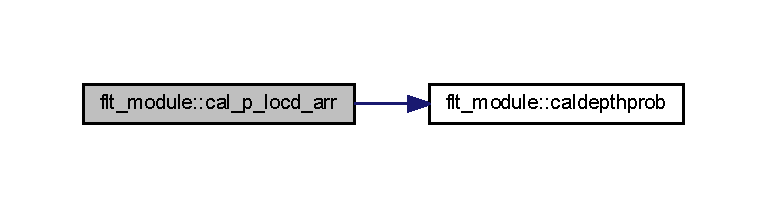
\includegraphics[width=350pt]{namespaceflt__module_aea512cba753c29d842ade7e80af288dc_cgraph}
\end{center}
\end{figure}


\hypertarget{namespaceflt__module_abdb1848f76f2f97490cbb813742463bb}{}\index{flt\+\_\+module@{flt\+\_\+module}!caldepthprob@{caldepthprob}}
\index{caldepthprob@{caldepthprob}!flt\+\_\+module@{flt\+\_\+module}}
\subsubsection[{caldepthprob()}]{\setlength{\rightskip}{0pt plus 5cm}subroutine flt\+\_\+module\+::caldepthprob (
\begin{DoxyParamCaption}
{}
\end{DoxyParamCaption}
)}\label{namespaceflt__module_abdb1848f76f2f97490cbb813742463bb}
\hypertarget{namespaceflt__module_a7c28beda425cae19654ab1d770575fa9}{}\index{flt\+\_\+module@{flt\+\_\+module}!deg2km\+\_\+model@{deg2km\+\_\+model}}
\index{deg2km\+\_\+model@{deg2km\+\_\+model}!flt\+\_\+module@{flt\+\_\+module}}
\subsubsection[{deg2km\+\_\+model()}]{\setlength{\rightskip}{0pt plus 5cm}subroutine flt\+\_\+module\+::deg2km\+\_\+model (
\begin{DoxyParamCaption}
{}
\end{DoxyParamCaption}
)}\label{namespaceflt__module_a7c28beda425cae19654ab1d770575fa9}


Here is the call graph for this function\+:
\nopagebreak
\begin{figure}[H]
\begin{center}
\leavevmode
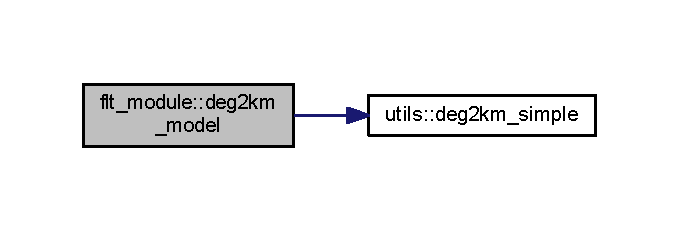
\includegraphics[width=326pt]{namespaceflt__module_a7c28beda425cae19654ab1d770575fa9_cgraph}
\end{center}
\end{figure}


\hypertarget{namespaceflt__module_a70e82d6c4a8cbb15e934c5b846b3f2fd}{}\index{flt\+\_\+module@{flt\+\_\+module}!flt\+\_\+ini@{flt\+\_\+ini}}
\index{flt\+\_\+ini@{flt\+\_\+ini}!flt\+\_\+module@{flt\+\_\+module}}
\subsubsection[{flt\+\_\+ini()}]{\setlength{\rightskip}{0pt plus 5cm}subroutine flt\+\_\+module\+::flt\+\_\+ini (
\begin{DoxyParamCaption}
{}
\end{DoxyParamCaption}
)}\label{namespaceflt__module_a70e82d6c4a8cbb15e934c5b846b3f2fd}


Here is the call graph for this function\+:
\nopagebreak
\begin{figure}[H]
\begin{center}
\leavevmode
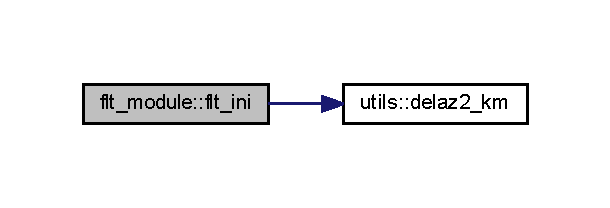
\includegraphics[width=293pt]{namespaceflt__module_a70e82d6c4a8cbb15e934c5b846b3f2fd_cgraph}
\end{center}
\end{figure}


\hypertarget{namespaceflt__module_a4df7cbbee97b24416c4834d0da1d86f5}{}\index{flt\+\_\+module@{flt\+\_\+module}!locate\+\_\+rupture@{locate\+\_\+rupture}}
\index{locate\+\_\+rupture@{locate\+\_\+rupture}!flt\+\_\+module@{flt\+\_\+module}}
\subsubsection[{locate\+\_\+rupture(\+S1\+\_\+local, S2\+\_\+local, rup\+\_\+coor)}]{\setlength{\rightskip}{0pt plus 5cm}subroutine flt\+\_\+module\+::locate\+\_\+rupture (
\begin{DoxyParamCaption}
\item[{real(8), intent(in)}]{S1\+\_\+local, }
\item[{real(8), intent(in)}]{S2\+\_\+local, }
\item[{real(8), dimension(\+:,\+:), intent(out), allocatable}]{rup\+\_\+coor}
\end{DoxyParamCaption}
)}\label{namespaceflt__module_a4df7cbbee97b24416c4834d0da1d86f5}
\hypertarget{namespaceflt__module_a36fbe983f26cb385897a0f3b3a69b374}{}\index{flt\+\_\+module@{flt\+\_\+module}!mag\+\_\+freq\+\_\+distribution@{mag\+\_\+freq\+\_\+distribution}}
\index{mag\+\_\+freq\+\_\+distribution@{mag\+\_\+freq\+\_\+distribution}!flt\+\_\+module@{flt\+\_\+module}}
\subsubsection[{mag\+\_\+freq\+\_\+distribution()}]{\setlength{\rightskip}{0pt plus 5cm}subroutine flt\+\_\+module\+::mag\+\_\+freq\+\_\+distribution (
\begin{DoxyParamCaption}
{}
\end{DoxyParamCaption}
)}\label{namespaceflt__module_a36fbe983f26cb385897a0f3b3a69b374}


Here is the call graph for this function\+:
\nopagebreak
\begin{figure}[H]
\begin{center}
\leavevmode
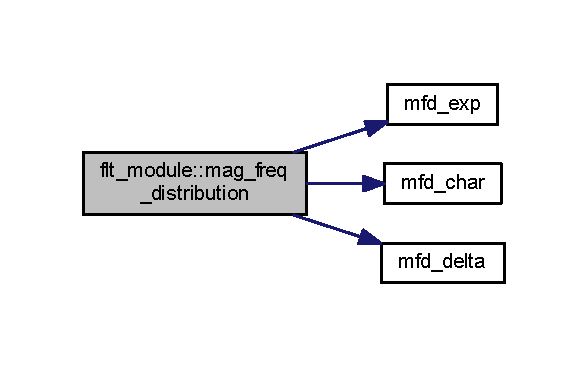
\includegraphics[width=282pt]{namespaceflt__module_a36fbe983f26cb385897a0f3b3a69b374_cgraph}
\end{center}
\end{figure}


\hypertarget{namespaceflt__module_a03121e683f2ec0d996e20de582b4a47c}{}\index{flt\+\_\+module@{flt\+\_\+module}!mw2arup@{mw2arup}}
\index{mw2arup@{mw2arup}!flt\+\_\+module@{flt\+\_\+module}}
\subsubsection[{mw2arup()}]{\setlength{\rightskip}{0pt plus 5cm}subroutine flt\+\_\+module\+::mw2arup (
\begin{DoxyParamCaption}
{}
\end{DoxyParamCaption}
)}\label{namespaceflt__module_a03121e683f2ec0d996e20de582b4a47c}
\hypertarget{namespaceflt__module_a5e554053b0a794d5027652daae033cbb}{}\index{flt\+\_\+module@{flt\+\_\+module}!rupture\+\_\+location@{rupture\+\_\+location}}
\index{rupture\+\_\+location@{rupture\+\_\+location}!flt\+\_\+module@{flt\+\_\+module}}
\subsubsection[{rupture\+\_\+location()}]{\setlength{\rightskip}{0pt plus 5cm}subroutine flt\+\_\+module\+::rupture\+\_\+location (
\begin{DoxyParamCaption}
{}
\end{DoxyParamCaption}
)}\label{namespaceflt__module_a5e554053b0a794d5027652daae033cbb}


Here is the call graph for this function\+:
\nopagebreak
\begin{figure}[H]
\begin{center}
\leavevmode
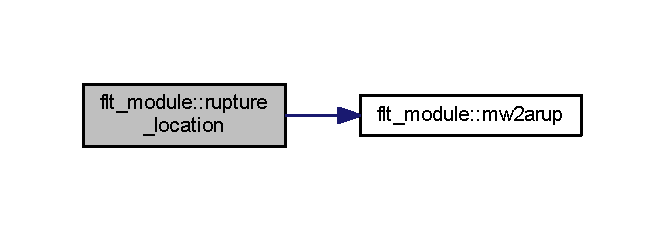
\includegraphics[width=319pt]{namespaceflt__module_a5e554053b0a794d5027652daae033cbb_cgraph}
\end{center}
\end{figure}


\hypertarget{namespaceflt__module_adf3a48955b957b3900c168b85a7e3a7f}{}\index{flt\+\_\+module@{flt\+\_\+module}!unit\+\_\+conversion@{unit\+\_\+conversion}}
\index{unit\+\_\+conversion@{unit\+\_\+conversion}!flt\+\_\+module@{flt\+\_\+module}}
\subsubsection[{unit\+\_\+conversion()}]{\setlength{\rightskip}{0pt plus 5cm}subroutine flt\+\_\+module\+::unit\+\_\+conversion (
\begin{DoxyParamCaption}
{}
\end{DoxyParamCaption}
)}\label{namespaceflt__module_adf3a48955b957b3900c168b85a7e3a7f}


Here is the call graph for this function\+:
\nopagebreak
\begin{figure}[H]
\begin{center}
\leavevmode
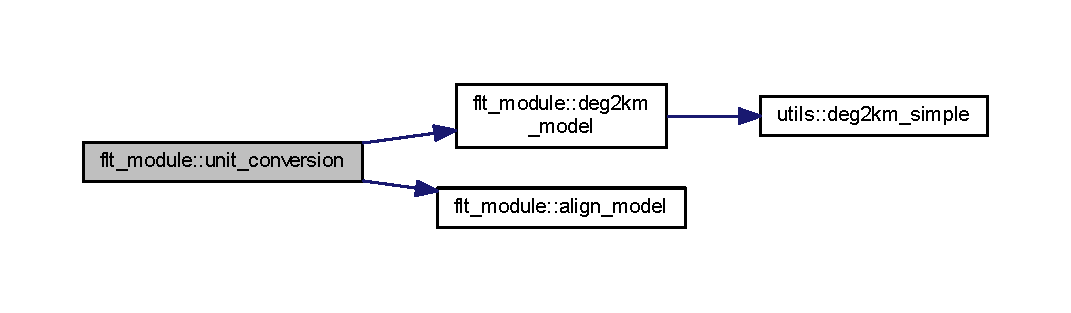
\includegraphics[width=350pt]{namespaceflt__module_adf3a48955b957b3900c168b85a7e3a7f_cgraph}
\end{center}
\end{figure}




\subsection{Variable Documentation}
\hypertarget{namespaceflt__module_a46387202eab4affb664fabc1dfbc3523}{}\index{flt\+\_\+module@{flt\+\_\+module}!coor\+\_\+d@{coor\+\_\+d}}
\index{coor\+\_\+d@{coor\+\_\+d}!flt\+\_\+module@{flt\+\_\+module}}
\subsubsection[{coor\+\_\+d}]{\setlength{\rightskip}{0pt plus 5cm}real(8), dimension(\+:,\+:), allocatable flt\+\_\+module\+::coor\+\_\+d}\label{namespaceflt__module_a46387202eab4affb664fabc1dfbc3523}
\hypertarget{namespaceflt__module_a5afcf609fce08da82c3c6f3c6ae623d1}{}\index{flt\+\_\+module@{flt\+\_\+module}!flt\+\_\+area@{flt\+\_\+area}}
\index{flt\+\_\+area@{flt\+\_\+area}!flt\+\_\+module@{flt\+\_\+module}}
\subsubsection[{flt\+\_\+area}]{\setlength{\rightskip}{0pt plus 5cm}real(8) flt\+\_\+module\+::flt\+\_\+area}\label{namespaceflt__module_a5afcf609fce08da82c3c6f3c6ae623d1}
\hypertarget{namespaceflt__module_afe7ee1528f7162ad84a3517be2962885}{}\index{flt\+\_\+module@{flt\+\_\+module}!flt\+\_\+az\+\_\+seg@{flt\+\_\+az\+\_\+seg}}
\index{flt\+\_\+az\+\_\+seg@{flt\+\_\+az\+\_\+seg}!flt\+\_\+module@{flt\+\_\+module}}
\subsubsection[{flt\+\_\+az\+\_\+seg}]{\setlength{\rightskip}{0pt plus 5cm}real(8), dimension(\+:), allocatable flt\+\_\+module\+::flt\+\_\+az\+\_\+seg}\label{namespaceflt__module_afe7ee1528f7162ad84a3517be2962885}
\hypertarget{namespaceflt__module_a5f040c388185e1ef250084d5c59d41e9}{}\index{flt\+\_\+module@{flt\+\_\+module}!flt\+\_\+coor@{flt\+\_\+coor}}
\index{flt\+\_\+coor@{flt\+\_\+coor}!flt\+\_\+module@{flt\+\_\+module}}
\subsubsection[{flt\+\_\+coor}]{\setlength{\rightskip}{0pt plus 5cm}real(8), dimension(\+:,\+:), allocatable flt\+\_\+module\+::flt\+\_\+coor}\label{namespaceflt__module_a5f040c388185e1ef250084d5c59d41e9}
\hypertarget{namespaceflt__module_a4bc1d05951c8d1ad1263099b2168fc52}{}\index{flt\+\_\+module@{flt\+\_\+module}!flt\+\_\+len@{flt\+\_\+len}}
\index{flt\+\_\+len@{flt\+\_\+len}!flt\+\_\+module@{flt\+\_\+module}}
\subsubsection[{flt\+\_\+len}]{\setlength{\rightskip}{0pt plus 5cm}real(8) flt\+\_\+module\+::flt\+\_\+len}\label{namespaceflt__module_a4bc1d05951c8d1ad1263099b2168fc52}
\hypertarget{namespaceflt__module_aca5726712ea516198b181e7cb2f58a79}{}\index{flt\+\_\+module@{flt\+\_\+module}!flt\+\_\+len\+\_\+seg@{flt\+\_\+len\+\_\+seg}}
\index{flt\+\_\+len\+\_\+seg@{flt\+\_\+len\+\_\+seg}!flt\+\_\+module@{flt\+\_\+module}}
\subsubsection[{flt\+\_\+len\+\_\+seg}]{\setlength{\rightskip}{0pt plus 5cm}real(8), dimension(\+:), allocatable flt\+\_\+module\+::flt\+\_\+len\+\_\+seg}\label{namespaceflt__module_aca5726712ea516198b181e7cb2f58a79}
\hypertarget{namespaceflt__module_ade0f97d7261ffc38567aa16de68c1583}{}\index{flt\+\_\+module@{flt\+\_\+module}!flt\+\_\+s\+\_\+corner@{flt\+\_\+s\+\_\+corner}}
\index{flt\+\_\+s\+\_\+corner@{flt\+\_\+s\+\_\+corner}!flt\+\_\+module@{flt\+\_\+module}}
\subsubsection[{flt\+\_\+s\+\_\+corner}]{\setlength{\rightskip}{0pt plus 5cm}real(8), dimension(\+:), allocatable flt\+\_\+module\+::flt\+\_\+s\+\_\+corner}\label{namespaceflt__module_ade0f97d7261ffc38567aa16de68c1583}
\hypertarget{namespaceflt__module_a5f628ae600d8550ab693d874d7a26bb0}{}\index{flt\+\_\+module@{flt\+\_\+module}!flt\+\_\+strike\+\_\+deg@{flt\+\_\+strike\+\_\+deg}}
\index{flt\+\_\+strike\+\_\+deg@{flt\+\_\+strike\+\_\+deg}!flt\+\_\+module@{flt\+\_\+module}}
\subsubsection[{flt\+\_\+strike\+\_\+deg}]{\setlength{\rightskip}{0pt plus 5cm}real(8) flt\+\_\+module\+::flt\+\_\+strike\+\_\+deg}\label{namespaceflt__module_a5f628ae600d8550ab693d874d7a26bb0}
\hypertarget{namespaceflt__module_a618a9014909e559bdbedf80be8a159a3}{}\index{flt\+\_\+module@{flt\+\_\+module}!flt\+\_\+strike\+\_\+rad@{flt\+\_\+strike\+\_\+rad}}
\index{flt\+\_\+strike\+\_\+rad@{flt\+\_\+strike\+\_\+rad}!flt\+\_\+module@{flt\+\_\+module}}
\subsubsection[{flt\+\_\+strike\+\_\+rad}]{\setlength{\rightskip}{0pt plus 5cm}real(8) flt\+\_\+module\+::flt\+\_\+strike\+\_\+rad}\label{namespaceflt__module_a618a9014909e559bdbedf80be8a159a3}
\hypertarget{namespaceflt__module_a0a0ca2180f3d4b230a85f4e74898c1ab}{}\index{flt\+\_\+module@{flt\+\_\+module}!flt\+\_\+wid@{flt\+\_\+wid}}
\index{flt\+\_\+wid@{flt\+\_\+wid}!flt\+\_\+module@{flt\+\_\+module}}
\subsubsection[{flt\+\_\+wid}]{\setlength{\rightskip}{0pt plus 5cm}real(8) flt\+\_\+module\+::flt\+\_\+wid}\label{namespaceflt__module_a0a0ca2180f3d4b230a85f4e74898c1ab}
\hypertarget{namespaceflt__module_a9e6d611f8124986d8547149562e07e40}{}\index{flt\+\_\+module@{flt\+\_\+module}!ftop@{ftop}}
\index{ftop@{ftop}!flt\+\_\+module@{flt\+\_\+module}}
\subsubsection[{ftop}]{\setlength{\rightskip}{0pt plus 5cm}real(8) flt\+\_\+module\+::ftop}\label{namespaceflt__module_a9e6d611f8124986d8547149562e07e40}
\hypertarget{namespaceflt__module_a9480fc2f60b62f2eb903d45f90e0dc73}{}\index{flt\+\_\+module@{flt\+\_\+module}!i\+\_\+dist\+\_\+bin@{i\+\_\+dist\+\_\+bin}}
\index{i\+\_\+dist\+\_\+bin@{i\+\_\+dist\+\_\+bin}!flt\+\_\+module@{flt\+\_\+module}}
\subsubsection[{i\+\_\+dist\+\_\+bin}]{\setlength{\rightskip}{0pt plus 5cm}integer flt\+\_\+module\+::i\+\_\+dist\+\_\+bin}\label{namespaceflt__module_a9480fc2f60b62f2eb903d45f90e0dc73}
\hypertarget{namespaceflt__module_a4bb764374a373b9dea720cedee5f208a}{}\index{flt\+\_\+module@{flt\+\_\+module}!i\+\_\+eps\+\_\+bin@{i\+\_\+eps\+\_\+bin}}
\index{i\+\_\+eps\+\_\+bin@{i\+\_\+eps\+\_\+bin}!flt\+\_\+module@{flt\+\_\+module}}
\subsubsection[{i\+\_\+eps\+\_\+bin}]{\setlength{\rightskip}{0pt plus 5cm}integer flt\+\_\+module\+::i\+\_\+eps\+\_\+bin}\label{namespaceflt__module_a4bb764374a373b9dea720cedee5f208a}
\hypertarget{namespaceflt__module_aa1dd9d9c50f40c03cb2d3e6772366e77}{}\index{flt\+\_\+module@{flt\+\_\+module}!i\+\_\+freq@{i\+\_\+freq}}
\index{i\+\_\+freq@{i\+\_\+freq}!flt\+\_\+module@{flt\+\_\+module}}
\subsubsection[{i\+\_\+freq}]{\setlength{\rightskip}{0pt plus 5cm}integer flt\+\_\+module\+::i\+\_\+freq}\label{namespaceflt__module_aa1dd9d9c50f40c03cb2d3e6772366e77}
\hypertarget{namespaceflt__module_ae179cb5e3d011707ce0742d9c49df852}{}\index{flt\+\_\+module@{flt\+\_\+module}!i\+\_\+inten@{i\+\_\+inten}}
\index{i\+\_\+inten@{i\+\_\+inten}!flt\+\_\+module@{flt\+\_\+module}}
\subsubsection[{i\+\_\+inten}]{\setlength{\rightskip}{0pt plus 5cm}integer flt\+\_\+module\+::i\+\_\+inten}\label{namespaceflt__module_ae179cb5e3d011707ce0742d9c49df852}
\hypertarget{namespaceflt__module_ab114b19843b4c7f6c795898a67157717}{}\index{flt\+\_\+module@{flt\+\_\+module}!i\+\_\+locd@{i\+\_\+locd}}
\index{i\+\_\+locd@{i\+\_\+locd}!flt\+\_\+module@{flt\+\_\+module}}
\subsubsection[{i\+\_\+locd}]{\setlength{\rightskip}{0pt plus 5cm}integer flt\+\_\+module\+::i\+\_\+locd}\label{namespaceflt__module_ab114b19843b4c7f6c795898a67157717}
\hypertarget{namespaceflt__module_ab04ec1f028778d49315cb1d0f6e80941}{}\index{flt\+\_\+module@{flt\+\_\+module}!i\+\_\+locs@{i\+\_\+locs}}
\index{i\+\_\+locs@{i\+\_\+locs}!flt\+\_\+module@{flt\+\_\+module}}
\subsubsection[{i\+\_\+locs}]{\setlength{\rightskip}{0pt plus 5cm}integer flt\+\_\+module\+::i\+\_\+locs}\label{namespaceflt__module_ab04ec1f028778d49315cb1d0f6e80941}
\hypertarget{namespaceflt__module_a5e6a726815330fe30804c2cfb77e2651}{}\index{flt\+\_\+module@{flt\+\_\+module}!i\+\_\+mag@{i\+\_\+mag}}
\index{i\+\_\+mag@{i\+\_\+mag}!flt\+\_\+module@{flt\+\_\+module}}
\subsubsection[{i\+\_\+mag}]{\setlength{\rightskip}{0pt plus 5cm}integer flt\+\_\+module\+::i\+\_\+mag}\label{namespaceflt__module_a5e6a726815330fe30804c2cfb77e2651}
\hypertarget{namespaceflt__module_a922b2ed6f3dff53fad4a824cde4270fd}{}\index{flt\+\_\+module@{flt\+\_\+module}!i\+\_\+mag\+\_\+bin@{i\+\_\+mag\+\_\+bin}}
\index{i\+\_\+mag\+\_\+bin@{i\+\_\+mag\+\_\+bin}!flt\+\_\+module@{flt\+\_\+module}}
\subsubsection[{i\+\_\+mag\+\_\+bin}]{\setlength{\rightskip}{0pt plus 5cm}integer flt\+\_\+module\+::i\+\_\+mag\+\_\+bin}\label{namespaceflt__module_a922b2ed6f3dff53fad4a824cde4270fd}
\hypertarget{namespaceflt__module_a74639d2c8f137bceff8db7f162301d8c}{}\index{flt\+\_\+module@{flt\+\_\+module}!i\+\_\+seg@{i\+\_\+seg}}
\index{i\+\_\+seg@{i\+\_\+seg}!flt\+\_\+module@{flt\+\_\+module}}
\subsubsection[{i\+\_\+seg}]{\setlength{\rightskip}{0pt plus 5cm}integer flt\+\_\+module\+::i\+\_\+seg}\label{namespaceflt__module_a74639d2c8f137bceff8db7f162301d8c}
\hypertarget{namespaceflt__module_af9892b4dca9fdd6644278654eb95f0d2}{}\index{flt\+\_\+module@{flt\+\_\+module}!mag\+\_\+inc@{mag\+\_\+inc}}
\index{mag\+\_\+inc@{mag\+\_\+inc}!flt\+\_\+module@{flt\+\_\+module}}
\subsubsection[{mag\+\_\+inc}]{\setlength{\rightskip}{0pt plus 5cm}real(8), dimension(\+:), allocatable flt\+\_\+module\+::mag\+\_\+inc}\label{namespaceflt__module_af9892b4dca9fdd6644278654eb95f0d2}
\hypertarget{namespaceflt__module_a758f2d6ebaadfe7af02eddd7ab5e4bdd}{}\index{flt\+\_\+module@{flt\+\_\+module}!mag\+\_\+inc\+\_\+0@{mag\+\_\+inc\+\_\+0}}
\index{mag\+\_\+inc\+\_\+0@{mag\+\_\+inc\+\_\+0}!flt\+\_\+module@{flt\+\_\+module}}
\subsubsection[{mag\+\_\+inc\+\_\+0}]{\setlength{\rightskip}{0pt plus 5cm}real(8), dimension(\+:), allocatable flt\+\_\+module\+::mag\+\_\+inc\+\_\+0}\label{namespaceflt__module_a758f2d6ebaadfe7af02eddd7ab5e4bdd}
\hypertarget{namespaceflt__module_aa0b3754bd3b678669c3b99f861359208}{}\index{flt\+\_\+module@{flt\+\_\+module}!mw@{mw}}
\index{mw@{mw}!flt\+\_\+module@{flt\+\_\+module}}
\subsubsection[{mw}]{\setlength{\rightskip}{0pt plus 5cm}real(8) flt\+\_\+module\+::mw}\label{namespaceflt__module_aa0b3754bd3b678669c3b99f861359208}
\hypertarget{namespaceflt__module_ab23ea8eb58ad8e18929cf668eb01f663}{}\index{flt\+\_\+module@{flt\+\_\+module}!n\+\_\+cor@{n\+\_\+cor}}
\index{n\+\_\+cor@{n\+\_\+cor}!flt\+\_\+module@{flt\+\_\+module}}
\subsubsection[{n\+\_\+cor}]{\setlength{\rightskip}{0pt plus 5cm}integer flt\+\_\+module\+::n\+\_\+cor}\label{namespaceflt__module_ab23ea8eb58ad8e18929cf668eb01f663}
\hypertarget{namespaceflt__module_a82fbb8ec3230fb344b2e8970e95398e3}{}\index{flt\+\_\+module@{flt\+\_\+module}!n\+\_\+locd@{n\+\_\+locd}}
\index{n\+\_\+locd@{n\+\_\+locd}!flt\+\_\+module@{flt\+\_\+module}}
\subsubsection[{n\+\_\+locd}]{\setlength{\rightskip}{0pt plus 5cm}integer flt\+\_\+module\+::n\+\_\+locd}\label{namespaceflt__module_a82fbb8ec3230fb344b2e8970e95398e3}
\hypertarget{namespaceflt__module_a544a94f997804736b60b9989c7489732}{}\index{flt\+\_\+module@{flt\+\_\+module}!n\+\_\+locs@{n\+\_\+locs}}
\index{n\+\_\+locs@{n\+\_\+locs}!flt\+\_\+module@{flt\+\_\+module}}
\subsubsection[{n\+\_\+locs}]{\setlength{\rightskip}{0pt plus 5cm}integer flt\+\_\+module\+::n\+\_\+locs}\label{namespaceflt__module_a544a94f997804736b60b9989c7489732}
\hypertarget{namespaceflt__module_ac480b7d0327ba835996ed5a35a3c6ec4}{}\index{flt\+\_\+module@{flt\+\_\+module}!n\+\_\+mag@{n\+\_\+mag}}
\index{n\+\_\+mag@{n\+\_\+mag}!flt\+\_\+module@{flt\+\_\+module}}
\subsubsection[{n\+\_\+mag}]{\setlength{\rightskip}{0pt plus 5cm}integer flt\+\_\+module\+::n\+\_\+mag}\label{namespaceflt__module_ac480b7d0327ba835996ed5a35a3c6ec4}
\hypertarget{namespaceflt__module_a9a55926b369374d66caf682a539d8acf}{}\index{flt\+\_\+module@{flt\+\_\+module}!p\+\_\+locd@{p\+\_\+locd}}
\index{p\+\_\+locd@{p\+\_\+locd}!flt\+\_\+module@{flt\+\_\+module}}
\subsubsection[{p\+\_\+locd}]{\setlength{\rightskip}{0pt plus 5cm}real(8) flt\+\_\+module\+::p\+\_\+locd}\label{namespaceflt__module_a9a55926b369374d66caf682a539d8acf}
\hypertarget{namespaceflt__module_a3ae9412ace7bafcdc16443a1de523c08}{}\index{flt\+\_\+module@{flt\+\_\+module}!p\+\_\+locd\+\_\+arr@{p\+\_\+locd\+\_\+arr}}
\index{p\+\_\+locd\+\_\+arr@{p\+\_\+locd\+\_\+arr}!flt\+\_\+module@{flt\+\_\+module}}
\subsubsection[{p\+\_\+locd\+\_\+arr}]{\setlength{\rightskip}{0pt plus 5cm}real(8), dimension(\+:), allocatable flt\+\_\+module\+::p\+\_\+locd\+\_\+arr}\label{namespaceflt__module_a3ae9412ace7bafcdc16443a1de523c08}
\hypertarget{namespaceflt__module_ac1c817f0b45b42ee735df0300075b47e}{}\index{flt\+\_\+module@{flt\+\_\+module}!p\+\_\+locs@{p\+\_\+locs}}
\index{p\+\_\+locs@{p\+\_\+locs}!flt\+\_\+module@{flt\+\_\+module}}
\subsubsection[{p\+\_\+locs}]{\setlength{\rightskip}{0pt plus 5cm}real(8) flt\+\_\+module\+::p\+\_\+locs}\label{namespaceflt__module_ac1c817f0b45b42ee735df0300075b47e}
\hypertarget{namespaceflt__module_ac0a06739ec2f31f13ad0b2213797e9c7}{}\index{flt\+\_\+module@{flt\+\_\+module}!rate@{rate}}
\index{rate@{rate}!flt\+\_\+module@{flt\+\_\+module}}
\subsubsection[{rate}]{\setlength{\rightskip}{0pt plus 5cm}real(8) flt\+\_\+module\+::rate}\label{namespaceflt__module_ac0a06739ec2f31f13ad0b2213797e9c7}
\hypertarget{namespaceflt__module_af4abd22305b27392695e298e409485eb}{}\index{flt\+\_\+module@{flt\+\_\+module}!rate\+\_\+inc@{rate\+\_\+inc}}
\index{rate\+\_\+inc@{rate\+\_\+inc}!flt\+\_\+module@{flt\+\_\+module}}
\subsubsection[{rate\+\_\+inc}]{\setlength{\rightskip}{0pt plus 5cm}real(8), dimension(\+:), allocatable flt\+\_\+module\+::rate\+\_\+inc}\label{namespaceflt__module_af4abd22305b27392695e298e409485eb}
\hypertarget{namespaceflt__module_a3aa16b477093fff931adc3d47efb4391}{}\index{flt\+\_\+module@{flt\+\_\+module}!rate\+\_\+inc\+\_\+0@{rate\+\_\+inc\+\_\+0}}
\index{rate\+\_\+inc\+\_\+0@{rate\+\_\+inc\+\_\+0}!flt\+\_\+module@{flt\+\_\+module}}
\subsubsection[{rate\+\_\+inc\+\_\+0}]{\setlength{\rightskip}{0pt plus 5cm}real(8), dimension(\+:), allocatable flt\+\_\+module\+::rate\+\_\+inc\+\_\+0}\label{namespaceflt__module_a3aa16b477093fff931adc3d47efb4391}
\hypertarget{namespaceflt__module_a61bb108f64be27cd6e6b621bd0d2be66}{}\index{flt\+\_\+module@{flt\+\_\+module}!rjb@{rjb}}
\index{rjb@{rjb}!flt\+\_\+module@{flt\+\_\+module}}
\subsubsection[{rjb}]{\setlength{\rightskip}{0pt plus 5cm}real(8) flt\+\_\+module\+::rjb}\label{namespaceflt__module_a61bb108f64be27cd6e6b621bd0d2be66}
\hypertarget{namespaceflt__module_aacc666d4125c94c8ff0b54e1a6fac18b}{}\index{flt\+\_\+module@{flt\+\_\+module}!rrup@{rrup}}
\index{rrup@{rrup}!flt\+\_\+module@{flt\+\_\+module}}
\subsubsection[{rrup}]{\setlength{\rightskip}{0pt plus 5cm}real(8) flt\+\_\+module\+::rrup}\label{namespaceflt__module_aacc666d4125c94c8ff0b54e1a6fac18b}
\hypertarget{namespaceflt__module_aec90f89a37148a6fe2fa52df737b51ef}{}\index{flt\+\_\+module@{flt\+\_\+module}!rup\+\_\+area@{rup\+\_\+area}}
\index{rup\+\_\+area@{rup\+\_\+area}!flt\+\_\+module@{flt\+\_\+module}}
\subsubsection[{rup\+\_\+area}]{\setlength{\rightskip}{0pt plus 5cm}real(8) flt\+\_\+module\+::rup\+\_\+area}\label{namespaceflt__module_aec90f89a37148a6fe2fa52df737b51ef}
\hypertarget{namespaceflt__module_af824d404f5d8ef8f21222c648b493389}{}\index{flt\+\_\+module@{flt\+\_\+module}!rup\+\_\+area\+\_\+trial@{rup\+\_\+area\+\_\+trial}}
\index{rup\+\_\+area\+\_\+trial@{rup\+\_\+area\+\_\+trial}!flt\+\_\+module@{flt\+\_\+module}}
\subsubsection[{rup\+\_\+area\+\_\+trial}]{\setlength{\rightskip}{0pt plus 5cm}real(8) flt\+\_\+module\+::rup\+\_\+area\+\_\+trial}\label{namespaceflt__module_af824d404f5d8ef8f21222c648b493389}
\hypertarget{namespaceflt__module_afbf76baeddad45d761cc805c838b369a}{}\index{flt\+\_\+module@{flt\+\_\+module}!rup\+\_\+coor@{rup\+\_\+coor}}
\index{rup\+\_\+coor@{rup\+\_\+coor}!flt\+\_\+module@{flt\+\_\+module}}
\subsubsection[{rup\+\_\+coor}]{\setlength{\rightskip}{0pt plus 5cm}real(8), dimension(\+:,\+:), allocatable flt\+\_\+module\+::rup\+\_\+coor}\label{namespaceflt__module_afbf76baeddad45d761cc805c838b369a}
\hypertarget{namespaceflt__module_aa83583fdd38e91b447b8fbf1ae9f833c}{}\index{flt\+\_\+module@{flt\+\_\+module}!rup\+\_\+len@{rup\+\_\+len}}
\index{rup\+\_\+len@{rup\+\_\+len}!flt\+\_\+module@{flt\+\_\+module}}
\subsubsection[{rup\+\_\+len}]{\setlength{\rightskip}{0pt plus 5cm}real(8) flt\+\_\+module\+::rup\+\_\+len}\label{namespaceflt__module_aa83583fdd38e91b447b8fbf1ae9f833c}
\hypertarget{namespaceflt__module_acb649d537953bd575e6bbded75b6c99b}{}\index{flt\+\_\+module@{flt\+\_\+module}!rup\+\_\+len\+\_\+trial@{rup\+\_\+len\+\_\+trial}}
\index{rup\+\_\+len\+\_\+trial@{rup\+\_\+len\+\_\+trial}!flt\+\_\+module@{flt\+\_\+module}}
\subsubsection[{rup\+\_\+len\+\_\+trial}]{\setlength{\rightskip}{0pt plus 5cm}real(8) flt\+\_\+module\+::rup\+\_\+len\+\_\+trial}\label{namespaceflt__module_acb649d537953bd575e6bbded75b6c99b}
\hypertarget{namespaceflt__module_ab5c2fb389cfd0080d938d50ef55e28ef}{}\index{flt\+\_\+module@{flt\+\_\+module}!rup\+\_\+top@{rup\+\_\+top}}
\index{rup\+\_\+top@{rup\+\_\+top}!flt\+\_\+module@{flt\+\_\+module}}
\subsubsection[{rup\+\_\+top}]{\setlength{\rightskip}{0pt plus 5cm}real(8), dimension(\+:), allocatable flt\+\_\+module\+::rup\+\_\+top}\label{namespaceflt__module_ab5c2fb389cfd0080d938d50ef55e28ef}
\hypertarget{namespaceflt__module_a5cbe7cb918ea3ecbe35270bdcc9ab63d}{}\index{flt\+\_\+module@{flt\+\_\+module}!rup\+\_\+wid@{rup\+\_\+wid}}
\index{rup\+\_\+wid@{rup\+\_\+wid}!flt\+\_\+module@{flt\+\_\+module}}
\subsubsection[{rup\+\_\+wid}]{\setlength{\rightskip}{0pt plus 5cm}real(8) flt\+\_\+module\+::rup\+\_\+wid}\label{namespaceflt__module_a5cbe7cb918ea3ecbe35270bdcc9ab63d}
\hypertarget{namespaceflt__module_a6cefaab59a5e1f02e62505b132fe9384}{}\index{flt\+\_\+module@{flt\+\_\+module}!rup\+\_\+wid\+\_\+trial@{rup\+\_\+wid\+\_\+trial}}
\index{rup\+\_\+wid\+\_\+trial@{rup\+\_\+wid\+\_\+trial}!flt\+\_\+module@{flt\+\_\+module}}
\subsubsection[{rup\+\_\+wid\+\_\+trial}]{\setlength{\rightskip}{0pt plus 5cm}real(8) flt\+\_\+module\+::rup\+\_\+wid\+\_\+trial}\label{namespaceflt__module_a6cefaab59a5e1f02e62505b132fe9384}
\hypertarget{namespaceflt__module_a8fa2cff4d9d0c963d1d2e99f399211c5}{}\index{flt\+\_\+module@{flt\+\_\+module}!rx@{rx}}
\index{rx@{rx}!flt\+\_\+module@{flt\+\_\+module}}
\subsubsection[{rx}]{\setlength{\rightskip}{0pt plus 5cm}real(8) flt\+\_\+module\+::rx}\label{namespaceflt__module_a8fa2cff4d9d0c963d1d2e99f399211c5}
\hypertarget{namespaceflt__module_a388db17b48dfcaeb0b4c53d1a23f83b6}{}\index{flt\+\_\+module@{flt\+\_\+module}!s1@{s1}}
\index{s1@{s1}!flt\+\_\+module@{flt\+\_\+module}}
\subsubsection[{s1}]{\setlength{\rightskip}{0pt plus 5cm}real(8), dimension(\+:), allocatable flt\+\_\+module\+::s1}\label{namespaceflt__module_a388db17b48dfcaeb0b4c53d1a23f83b6}
\hypertarget{namespaceflt__module_a774958e9c5ad266c9faed76a724e27ac}{}\index{flt\+\_\+module@{flt\+\_\+module}!s2@{s2}}
\index{s2@{s2}!flt\+\_\+module@{flt\+\_\+module}}
\subsubsection[{s2}]{\setlength{\rightskip}{0pt plus 5cm}real(8), dimension(\+:), allocatable flt\+\_\+module\+::s2}\label{namespaceflt__module_a774958e9c5ad266c9faed76a724e27ac}
\hypertarget{namespaceflt__module_a2aeddbabcca2c320d94712a5ef502b79}{}\index{flt\+\_\+module@{flt\+\_\+module}!site\+\_\+coor@{site\+\_\+coor}}
\index{site\+\_\+coor@{site\+\_\+coor}!flt\+\_\+module@{flt\+\_\+module}}
\subsubsection[{site\+\_\+coor}]{\setlength{\rightskip}{0pt plus 5cm}real(8), dimension(2) flt\+\_\+module\+::site\+\_\+coor}\label{namespaceflt__module_a2aeddbabcca2c320d94712a5ef502b79}
\hypertarget{namespaceflt__module_ad4dbd8fe640ed7c127b993e51b31c2cb}{}\index{flt\+\_\+module@{flt\+\_\+module}!step\+\_\+d@{step\+\_\+d}}
\index{step\+\_\+d@{step\+\_\+d}!flt\+\_\+module@{flt\+\_\+module}}
\subsubsection[{step\+\_\+d}]{\setlength{\rightskip}{0pt plus 5cm}real(8) flt\+\_\+module\+::step\+\_\+d}\label{namespaceflt__module_ad4dbd8fe640ed7c127b993e51b31c2cb}
\hypertarget{namespaceflt__module_a2bbb6ee47643b88f63a980bf4f075ad5}{}\index{flt\+\_\+module@{flt\+\_\+module}!step\+\_\+d\+\_\+h@{step\+\_\+d\+\_\+h}}
\index{step\+\_\+d\+\_\+h@{step\+\_\+d\+\_\+h}!flt\+\_\+module@{flt\+\_\+module}}
\subsubsection[{step\+\_\+d\+\_\+h}]{\setlength{\rightskip}{0pt plus 5cm}real(8) flt\+\_\+module\+::step\+\_\+d\+\_\+h}\label{namespaceflt__module_a2bbb6ee47643b88f63a980bf4f075ad5}
\hypertarget{namespaceflt__module_afaa001d959f566926be3b2e7383fa244}{}\index{flt\+\_\+module@{flt\+\_\+module}!step\+\_\+d\+\_\+hc@{step\+\_\+d\+\_\+hc}}
\index{step\+\_\+d\+\_\+hc@{step\+\_\+d\+\_\+hc}!flt\+\_\+module@{flt\+\_\+module}}
\subsubsection[{step\+\_\+d\+\_\+hc}]{\setlength{\rightskip}{0pt plus 5cm}real(8) flt\+\_\+module\+::step\+\_\+d\+\_\+hc}\label{namespaceflt__module_afaa001d959f566926be3b2e7383fa244}
\hypertarget{namespaceflt__module_a5e5aaec050d5c1fa09b359dc2b162532}{}\index{flt\+\_\+module@{flt\+\_\+module}!step\+\_\+d\+\_\+hs@{step\+\_\+d\+\_\+hs}}
\index{step\+\_\+d\+\_\+hs@{step\+\_\+d\+\_\+hs}!flt\+\_\+module@{flt\+\_\+module}}
\subsubsection[{step\+\_\+d\+\_\+hs}]{\setlength{\rightskip}{0pt plus 5cm}real(8) flt\+\_\+module\+::step\+\_\+d\+\_\+hs}\label{namespaceflt__module_a5e5aaec050d5c1fa09b359dc2b162532}
\hypertarget{namespaceflt__module_a5a750dfe01760a5134b5cd98aa924b01}{}\index{flt\+\_\+module@{flt\+\_\+module}!step\+\_\+d\+\_\+trial@{step\+\_\+d\+\_\+trial}}
\index{step\+\_\+d\+\_\+trial@{step\+\_\+d\+\_\+trial}!flt\+\_\+module@{flt\+\_\+module}}
\subsubsection[{step\+\_\+d\+\_\+trial}]{\setlength{\rightskip}{0pt plus 5cm}real(8) flt\+\_\+module\+::step\+\_\+d\+\_\+trial}\label{namespaceflt__module_a5a750dfe01760a5134b5cd98aa924b01}
\hypertarget{namespaceflt__module_a3a9896b28d0823ab1f9c8bda7380c0d9}{}\index{flt\+\_\+module@{flt\+\_\+module}!step\+\_\+d\+\_\+v@{step\+\_\+d\+\_\+v}}
\index{step\+\_\+d\+\_\+v@{step\+\_\+d\+\_\+v}!flt\+\_\+module@{flt\+\_\+module}}
\subsubsection[{step\+\_\+d\+\_\+v}]{\setlength{\rightskip}{0pt plus 5cm}real(8) flt\+\_\+module\+::step\+\_\+d\+\_\+v}\label{namespaceflt__module_a3a9896b28d0823ab1f9c8bda7380c0d9}
\hypertarget{namespaceflt__module_aac3ac3d5dda31c71db0f70b6c04bde99}{}\index{flt\+\_\+module@{flt\+\_\+module}!step\+\_\+s@{step\+\_\+s}}
\index{step\+\_\+s@{step\+\_\+s}!flt\+\_\+module@{flt\+\_\+module}}
\subsubsection[{step\+\_\+s}]{\setlength{\rightskip}{0pt plus 5cm}real(8) flt\+\_\+module\+::step\+\_\+s}\label{namespaceflt__module_aac3ac3d5dda31c71db0f70b6c04bde99}
\hypertarget{namespaceflt__module_abbc6ad6d8104d02669bab58b22654f6b}{}\index{flt\+\_\+module@{flt\+\_\+module}!step\+\_\+s\+\_\+trial@{step\+\_\+s\+\_\+trial}}
\index{step\+\_\+s\+\_\+trial@{step\+\_\+s\+\_\+trial}!flt\+\_\+module@{flt\+\_\+module}}
\subsubsection[{step\+\_\+s\+\_\+trial}]{\setlength{\rightskip}{0pt plus 5cm}real(8) flt\+\_\+module\+::step\+\_\+s\+\_\+trial}\label{namespaceflt__module_abbc6ad6d8104d02669bab58b22654f6b}
\hypertarget{namespaceflt__module_ab88c9c308585340c18213d3778e152a9}{}\index{flt\+\_\+module@{flt\+\_\+module}!tin@{tin}}
\index{tin@{tin}!flt\+\_\+module@{flt\+\_\+module}}
\subsubsection[{tin}]{\setlength{\rightskip}{0pt plus 5cm}real(8) flt\+\_\+module\+::tin}\label{namespaceflt__module_ab88c9c308585340c18213d3778e152a9}

\hypertarget{namespacegmpe__module}{}\section{gmpe\+\_\+module Module Reference}
\label{namespacegmpe__module}\index{gmpe\+\_\+module@{gmpe\+\_\+module}}
\subsection*{Functions/\+Subroutines}
\begin{DoxyCompactItemize}
\item 
subroutine \hyperlink{namespacegmpe__module_a5f684874da41cb0160ab7c0473b1adf5}{gmpe\+\_\+interface} (m\+\_\+gmpe\+\_\+name, Tin, Mw, m\+\_\+sof, Rrup, Rjb, Rx, Ztor, dip,                                           Vs30, Z10, gmpe\+\_\+params, gmpe\+\_\+opts,                                           ln\+Sa, Sigma)
\item 
subroutine \hyperlink{namespacegmpe__module_a3a1c1fc463d12762d4dcc724f90f876d}{gmpe\+\_\+sadigh97} (ln\+Sa, Sigma, M, Rrup, Tin, m\+\_\+\+S\+O\+F)
\item 
subroutine \hyperlink{namespacegmpe__module_a908fe9e90b79ba090e108746e35b4b02}{gmpe\+\_\+cy14} (M, T, Rrup, Rjb, Rx, Ztor, dip, m\+\_\+\+S\+O\+F, Z10, Vs30, gmpe\+\_\+params, gmpe\+\_\+opts, ln\+Sa, sigma)
\item 
subroutine \hyperlink{namespacegmpe__module_a2b7ab2b80fab7e94cfd35a2e5652bc5a}{cy\+\_\+2014\+\_\+sub} (M, ip, R\+\_\+\+R\+U\+P, R\+\_\+\+J\+B, Rx, Ztor, delta, F\+\_\+\+R\+V, F\+\_\+\+N\+M, H\+W, Z10, Vs30, F\+V\+S30, region, d\+\_\+\+D\+P\+P, ln\+Sa, sigma)
\item 
subroutine \hyperlink{namespacegmpe__module_aaef04e7344731f519aba25dbde1bfbc8}{per\+\_\+indx\+\_\+cy14} (per, per\+\_\+indx)
\end{DoxyCompactItemize}


\subsection{Function/\+Subroutine Documentation}
\hypertarget{namespacegmpe__module_a2b7ab2b80fab7e94cfd35a2e5652bc5a}{}\index{gmpe\+\_\+module@{gmpe\+\_\+module}!cy\+\_\+2014\+\_\+sub@{cy\+\_\+2014\+\_\+sub}}
\index{cy\+\_\+2014\+\_\+sub@{cy\+\_\+2014\+\_\+sub}!gmpe\+\_\+module@{gmpe\+\_\+module}}
\subsubsection[{cy\+\_\+2014\+\_\+sub(\+M, ip, R\+\_\+\+R\+U\+P, R\+\_\+\+J\+B, Rx, Ztor, delta, F\+\_\+\+R\+V, F\+\_\+\+N\+M, H\+W, Z10, Vs30, F\+V\+S30, region, d\+\_\+\+D\+P\+P, ln\+Sa, sigma)}]{\setlength{\rightskip}{0pt plus 5cm}subroutine gmpe\+\_\+module\+::cy\+\_\+2014\+\_\+sub (
\begin{DoxyParamCaption}
\item[{real(8)}]{M, }
\item[{integer}]{ip, }
\item[{real(8)}]{R\+\_\+\+R\+U\+P, }
\item[{real(8)}]{R\+\_\+\+J\+B, }
\item[{real(8)}]{Rx, }
\item[{real(8)}]{Ztor, }
\item[{real(8)}]{delta, }
\item[{integer}]{F\+\_\+\+R\+V, }
\item[{integer}]{F\+\_\+\+N\+M, }
\item[{real(8)}]{H\+W, }
\item[{real(8)}]{Z10, }
\item[{real(8)}]{Vs30, }
\item[{integer}]{F\+V\+S30, }
\item[{integer}]{region, }
\item[{real(8)}]{d\+\_\+\+D\+P\+P, }
\item[{real(8)}]{ln\+Sa, }
\item[{real(8)}]{sigma}
\end{DoxyParamCaption}
)}\label{namespacegmpe__module_a2b7ab2b80fab7e94cfd35a2e5652bc5a}
\hypertarget{namespacegmpe__module_a908fe9e90b79ba090e108746e35b4b02}{}\index{gmpe\+\_\+module@{gmpe\+\_\+module}!gmpe\+\_\+cy14@{gmpe\+\_\+cy14}}
\index{gmpe\+\_\+cy14@{gmpe\+\_\+cy14}!gmpe\+\_\+module@{gmpe\+\_\+module}}
\subsubsection[{gmpe\+\_\+cy14(\+M, T, Rrup, Rjb, Rx, Ztor, dip, m\+\_\+\+S\+O\+F, Z10, Vs30, gmpe\+\_\+params, gmpe\+\_\+opts, ln\+Sa, sigma)}]{\setlength{\rightskip}{0pt plus 5cm}subroutine gmpe\+\_\+module\+::gmpe\+\_\+cy14 (
\begin{DoxyParamCaption}
\item[{real(8)}]{M, }
\item[{real(8)}]{T, }
\item[{real(8)}]{Rrup, }
\item[{real(8)}]{Rjb, }
\item[{real(8)}]{Rx, }
\item[{real(8)}]{Ztor, }
\item[{real(8)}]{dip, }
\item[{integer}]{m\+\_\+\+S\+O\+F, }
\item[{real(8)}]{Z10, }
\item[{real(8)}]{Vs30, }
\item[{real(8), dimension(\+:)}]{gmpe\+\_\+params, }
\item[{integer, dimension(\+:)}]{gmpe\+\_\+opts, }
\item[{real(8)}]{ln\+Sa, }
\item[{real(8)}]{sigma}
\end{DoxyParamCaption}
)}\label{namespacegmpe__module_a908fe9e90b79ba090e108746e35b4b02}


Here is the call graph for this function\+:
\nopagebreak
\begin{figure}[H]
\begin{center}
\leavevmode
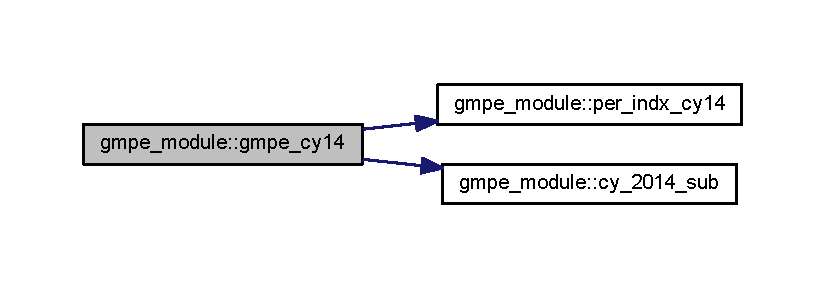
\includegraphics[width=350pt]{namespacegmpe__module_a908fe9e90b79ba090e108746e35b4b02_cgraph}
\end{center}
\end{figure}


\hypertarget{namespacegmpe__module_a5f684874da41cb0160ab7c0473b1adf5}{}\index{gmpe\+\_\+module@{gmpe\+\_\+module}!gmpe\+\_\+interface@{gmpe\+\_\+interface}}
\index{gmpe\+\_\+interface@{gmpe\+\_\+interface}!gmpe\+\_\+module@{gmpe\+\_\+module}}
\subsubsection[{gmpe\+\_\+interface(m\+\_\+gmpe\+\_\+name, Tin, Mw, m\+\_\+sof, Rrup, Rjb, Rx, Ztor, dip,                                           Vs30, Z10, gmpe\+\_\+params, gmpe\+\_\+opts,                                           ln\+Sa, Sigma)}]{\setlength{\rightskip}{0pt plus 5cm}subroutine gmpe\+\_\+module\+::gmpe\+\_\+interface (
\begin{DoxyParamCaption}
\item[{integer}]{m\+\_\+gmpe\+\_\+name, }
\item[{real(8)}]{Tin, }
\item[{real(8)}]{Mw, }
\item[{integer}]{m\+\_\+sof, }
\item[{real(8)}]{Rrup, }
\item[{real(8)}]{Rjb, }
\item[{real(8)}]{Rx, }
\item[{real(8)}]{Ztor, }
\item[{real(8)}]{dip, }
\item[{real(8)}]{Vs30, }
\item[{real(8)}]{Z10, }
\item[{real(8), dimension(\+:), allocatable}]{gmpe\+\_\+params, }
\item[{integer, dimension(\+:), allocatable}]{gmpe\+\_\+opts, }
\item[{real(8)}]{ln\+Sa, }
\item[{real(8)}]{Sigma}
\end{DoxyParamCaption}
)}\label{namespacegmpe__module_a5f684874da41cb0160ab7c0473b1adf5}


Here is the call graph for this function\+:
\nopagebreak
\begin{figure}[H]
\begin{center}
\leavevmode
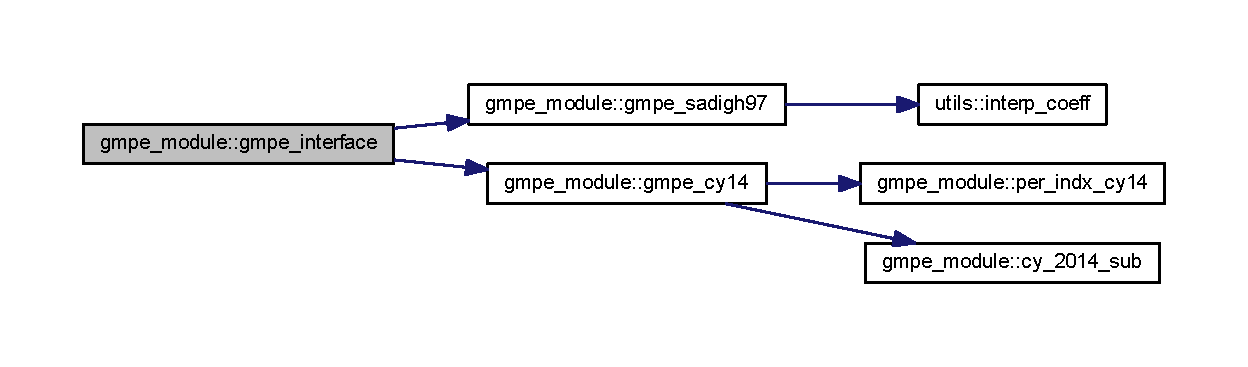
\includegraphics[width=350pt]{namespacegmpe__module_a5f684874da41cb0160ab7c0473b1adf5_cgraph}
\end{center}
\end{figure}


\hypertarget{namespacegmpe__module_a3a1c1fc463d12762d4dcc724f90f876d}{}\index{gmpe\+\_\+module@{gmpe\+\_\+module}!gmpe\+\_\+sadigh97@{gmpe\+\_\+sadigh97}}
\index{gmpe\+\_\+sadigh97@{gmpe\+\_\+sadigh97}!gmpe\+\_\+module@{gmpe\+\_\+module}}
\subsubsection[{gmpe\+\_\+sadigh97(ln\+Sa, Sigma, M, Rrup, Tin, m\+\_\+\+S\+O\+F)}]{\setlength{\rightskip}{0pt plus 5cm}subroutine gmpe\+\_\+module\+::gmpe\+\_\+sadigh97 (
\begin{DoxyParamCaption}
\item[{real(8)}]{ln\+Sa, }
\item[{real(8)}]{Sigma, }
\item[{real(8)}]{M, }
\item[{real(8)}]{Rrup, }
\item[{real(8)}]{Tin, }
\item[{integer}]{m\+\_\+\+S\+O\+F}
\end{DoxyParamCaption}
)}\label{namespacegmpe__module_a3a1c1fc463d12762d4dcc724f90f876d}


Here is the call graph for this function\+:
\nopagebreak
\begin{figure}[H]
\begin{center}
\leavevmode
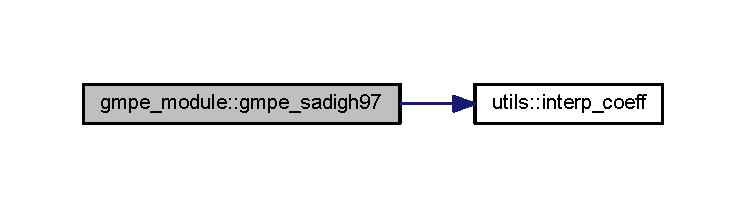
\includegraphics[width=350pt]{namespacegmpe__module_a3a1c1fc463d12762d4dcc724f90f876d_cgraph}
\end{center}
\end{figure}


\hypertarget{namespacegmpe__module_aaef04e7344731f519aba25dbde1bfbc8}{}\index{gmpe\+\_\+module@{gmpe\+\_\+module}!per\+\_\+indx\+\_\+cy14@{per\+\_\+indx\+\_\+cy14}}
\index{per\+\_\+indx\+\_\+cy14@{per\+\_\+indx\+\_\+cy14}!gmpe\+\_\+module@{gmpe\+\_\+module}}
\subsubsection[{per\+\_\+indx\+\_\+cy14(per, per\+\_\+indx)}]{\setlength{\rightskip}{0pt plus 5cm}subroutine gmpe\+\_\+module\+::per\+\_\+indx\+\_\+cy14 (
\begin{DoxyParamCaption}
\item[{real(8)}]{per, }
\item[{integer}]{per\+\_\+indx}
\end{DoxyParamCaption}
)}\label{namespacegmpe__module_aaef04e7344731f519aba25dbde1bfbc8}

\hypertarget{namespaceinput__module}{}\section{input\+\_\+module Module Reference}
\label{namespaceinput__module}\index{input\+\_\+module@{input\+\_\+module}}
\subsection*{Functions/\+Subroutines}
\begin{DoxyCompactItemize}
\item 
subroutine \hyperlink{namespaceinput__module_a00c4a5d066f42d27b85b05a38bed5160}{read\+\_\+input} ()
\item 
subroutine \hyperlink{namespaceinput__module_a07cd15a61e7f02633605f2f442ceb937}{read\+\_\+site} ()
\item 
subroutine \hyperlink{namespaceinput__module_afa2966a0e5fac1ac508ed7aed4f0a3d8}{read\+\_\+frequency} ()
\item 
subroutine \hyperlink{namespaceinput__module_a0d373b7166a3c84647da12172e1ea635}{read\+\_\+fault\+\_\+trace} ()
\item 
subroutine \hyperlink{namespaceinput__module_a1e706b509f806cf51ec52d88f6be16f5}{read\+\_\+rec\+\_\+relation} ()
\item 
subroutine \hyperlink{namespaceinput__module_a162c082b34aa3c082906be0b3260e07b}{read\+\_\+slip\+\_\+rate} ()
\item 
subroutine \hyperlink{namespaceinput__module_aeafdecc4d19831cf533fb2dcaf0a0844}{read\+\_\+b\+\_\+value} ()
\item 
subroutine \hyperlink{namespaceinput__module_acc844c5a0060bf20c9ae19ac3d2e3740}{read\+\_\+sof} ()
\item 
subroutine \hyperlink{namespaceinput__module_af0a24a3c1c27d7891b4ca97e8cbf73e8}{read\+\_\+unit} ()
\item 
subroutine \hyperlink{namespaceinput__module_a05356d7be39772919ba250f4ea4da2f3}{read\+\_\+aleatory\+\_\+distribution} ()
\item 
subroutine \hyperlink{namespaceinput__module_a57f855a995185ff6d52c0a402a4a536b}{read\+\_\+trunc\+\_\+level} ()
\item 
subroutine \hyperlink{namespaceinput__module_a0c45a351fde1aa9a3fe8f15c1d78330e}{read\+\_\+scaling\+\_\+model}
\item 
subroutine \hyperlink{namespaceinput__module_ac982cae54a9baa5626ed817f28c75595}{read\+\_\+dip} ()
\item 
subroutine \hyperlink{namespaceinput__module_a2b2d0311a6010b3b3e59cd947b58f429}{read\+\_\+gmpe\+\_\+name} ()
\item 
subroutine \hyperlink{namespaceinput__module_a4989c6ca8bc90648ca9587bee66d26b1}{read\+\_\+vs30} ()
\item 
subroutine \hyperlink{namespaceinput__module_a79ff648d45e7ac3f88ed461464c23901}{read\+\_\+z10} ()
\item 
subroutine \hyperlink{namespaceinput__module_a37d4fe4627c2f2d2f7063f9df9730476}{read\+\_\+z25} ()
\item 
subroutine \hyperlink{namespaceinput__module_a3b50bd9377741e86fbc4f43ec8e5ef93}{read\+\_\+seismogenic\+\_\+depth} ()
\item 
subroutine \hyperlink{namespaceinput__module_af139a93b520328955d0ff24a5283a948}{read\+\_\+depth\+\_\+distribution} ()
\item 
subroutine \hyperlink{namespaceinput__module_a2b52a667be52963438f117c68ae24bd1}{read\+\_\+aspect\+\_\+ratio} ()
\item 
subroutine \hyperlink{namespaceinput__module_a82104204d5b1aff59b087d4b87cf166b}{read\+\_\+strike\+\_\+dip\+\_\+step} ()
\item 
subroutine \hyperlink{namespaceinput__module_a9277ed03dfb00814405f98a5b0455d1c}{read\+\_\+mag\+\_\+range} ()
\item 
subroutine \hyperlink{namespaceinput__module_a7ce68361e26ec82b49e5313f235dc695}{read\+\_\+depth\+\_\+param} ()
\item 
subroutine \hyperlink{namespaceinput__module_a236da7bc51e5b4d79ef626a76b8dbea1}{read\+\_\+mag\+\_\+step} ()
\item 
subroutine \hyperlink{namespaceinput__module_acd40b5b88af0a4f619e2054305e670bb}{read\+\_\+intensity} ()
\item 
subroutine \hyperlink{namespaceinput__module_a9cf8432b15120af2d78057266ef67ae0}{read\+\_\+mag\+\_\+bin} ()
\item 
subroutine \hyperlink{namespaceinput__module_a8205f938072af7f3a84f190cdf9e32b3}{read\+\_\+dist\+\_\+bin} ()
\item 
subroutine \hyperlink{namespaceinput__module_a5d16b74f3e1993596b03be49827acd58}{read\+\_\+eps\+\_\+bin} ()
\item 
subroutine \hyperlink{namespaceinput__module_a86e724d27e380be85ae46ead8f422ab5}{read\+\_\+gmpe\+\_\+params} ()
\item 
subroutine \hyperlink{namespaceinput__module_ae5ed3783a3cd022cd1606bd280ca816d}{read\+\_\+gmpe\+\_\+opts} ()
\item 
subroutine \hyperlink{namespaceinput__module_a196ab42a030cc2c0efcd2bd463afa3f8}{close\+\_\+file} ()
\item 
subroutine \hyperlink{namespaceinput__module_ab34e9ffe1c6528cc2b5dc30c18126c11}{print\+\_\+haz\+\_\+bin} (haz\+\_\+bin)
\item 
subroutine \hyperlink{namespaceinput__module_a8dca2c193a492040a82753e06385b154}{print\+\_\+haz} (haz)
\end{DoxyCompactItemize}
\subsection*{Variables}
\begin{DoxyCompactItemize}
\item 
integer \hyperlink{namespaceinput__module_a7d1f1dd6198e0770d9218a80115df0de}{fp\+\_\+inp}
\item 
integer \hyperlink{namespaceinput__module_a24121f5e413cdf763ada92cb0c916ba3}{fp\+\_\+log}
\item 
integer \hyperlink{namespaceinput__module_a5b74d4c157160f6d6eaef2c725b02d6a}{fp\+\_\+haz}
\item 
integer \hyperlink{namespaceinput__module_a52ffef6eb6299a12612cc0b2eb5352dc}{fp\+\_\+dag}
\item 
integer \hyperlink{namespaceinput__module_a73158a89ce75123f19e014408bb9b342}{fp\+\_\+rup}
\item 
integer \hyperlink{namespaceinput__module_a34271f9a9a4c0c0d531db4d9e2b05fc3}{ppos}
\item 
logical \hyperlink{namespaceinput__module_af09923ed6808263d4497c13126abdb46}{inp\+\_\+exist}
\item 
character(130) \hyperlink{namespaceinput__module_ad228ac099c1afd318803f2d8514dd2c9}{fnm\+\_\+inp}
\item 
character(130) \hyperlink{namespaceinput__module_a7f573d3c228f74f193a801e6cb1175ef}{arg}
\item 
character(130) \hyperlink{namespaceinput__module_a95df80960079d35b95016b2448da8dcc}{fnm\+\_\+log}
\item 
character(130) \hyperlink{namespaceinput__module_ab37b626c8a9c8a0ad42d001c9a0e5ac4}{fnm\+\_\+haz}
\item 
character(130) \hyperlink{namespaceinput__module_ae99c24908c83beaac79f68a46d079e37}{fnm\+\_\+dag}
\item 
character(130) \hyperlink{namespaceinput__module_a913978d3f2a95df35b24c099c6599cd0}{fnm\+\_\+rup}
\item 
integer \hyperlink{namespaceinput__module_ada333752feb1551085c3d0331da41a6d}{eastat}
\item 
integer \hyperlink{namespaceinput__module_a865cd5e2924fbc40aeefe8bcb6226a75}{iost}
\item 
character(130) \hyperlink{namespaceinput__module_a304ebe11a9b47adcaeb6db5be6bae12d}{line}
\item 
character(130) \hyperlink{namespaceinput__module_ae257590e746cae45e031d04017cf76d1}{wrt\+\_\+fmt}
\item 
character(130) \hyperlink{namespaceinput__module_aa2d7dcffb5650145aa835a858a0ad35a}{str\+\_\+tmp}
\item 
character(130) \hyperlink{namespaceinput__module_ae241dcd6d1b9e390d39acb1f7ed2f38b}{gmpe\+\_\+name}
\item 
character(3) \hyperlink{namespaceinput__module_a781c43885db3614608686197e48ab56b}{ext\+\_\+log} = \textquotesingle{}log\textquotesingle{}
\item 
character(3) \hyperlink{namespaceinput__module_a860f66b4ca95c52a45651e1a7033e302}{ext\+\_\+haz} = \textquotesingle{}haz\textquotesingle{}
\item 
character(3) \hyperlink{namespaceinput__module_ab8a4b6a5af6ac707c4c8656e4d709bec}{ext\+\_\+dag} = \textquotesingle{}dag\textquotesingle{}
\item 
character(3) \hyperlink{namespaceinput__module_a5ba0c6f56b537efe7105ffc5ef3a9a98}{ext\+\_\+rup} = \textquotesingle{}rup\textquotesingle{}
\item 
real(8), dimension(2) \hyperlink{namespaceinput__module_ab574bddc682ceabd1271512c2b1f4e20}{site}
\item 
real(8), dimension(\+:), allocatable \hyperlink{namespaceinput__module_a2eec881a49e9f9d341e49f123b8435a3}{frequency}
\item 
real(8), dimension(\+:), allocatable \hyperlink{namespaceinput__module_ab8a5b4989aa8a656c28df7fa39f21d03}{intensity}
\item 
real(8), dimension(\+:), allocatable \hyperlink{namespaceinput__module_a1bbdfb734d8c5f5b6370d1ab7fbfb04a}{mag\+\_\+bin}
\item 
real(8), dimension(\+:), allocatable \hyperlink{namespaceinput__module_a760ea371c13a02c658f3ec689a63adad}{dist\+\_\+bin}
\item 
real(8), dimension(\+:), allocatable \hyperlink{namespaceinput__module_a6900d0ebf1a2f906895db37f5b82e495}{eps\+\_\+bin}
\item 
real(8), dimension(\+:,\+:), allocatable \hyperlink{namespaceinput__module_a289e412144c4ad26f482d664135f3972}{flt\+\_\+trace}
\item 
real(8), dimension(\+:), allocatable \hyperlink{namespaceinput__module_ab52a267c1d75b879ad598fa6cc377c4b}{gmpe\+\_\+params}
\item 
integer, dimension(\+:), allocatable \hyperlink{namespaceinput__module_a1c956fb0e5942428da3bdb0c932fd10c}{gmpe\+\_\+opts}
\item 
real(8), dimension(500, 2) \hyperlink{namespaceinput__module_ac72418d482bc6d9b164dc8ff77f80812}{temp2}
\item 
real(8), dimension(500) \hyperlink{namespaceinput__module_a35e70ed5e2a0858cd4af8970e6b7a3fe}{temp1}
\item 
integer, dimension(500) \hyperlink{namespaceinput__module_a129d3471a7d48a92476195ec540b0599}{temp\+\_\+int}
\item 
integer \hyperlink{namespaceinput__module_a98528ea542cc829033364307335ecdf6}{tmp\+\_\+int}
\item 
real(8) \hyperlink{namespaceinput__module_a1030c19aa6f6f484e8f538320aa753b0}{tmp1}
\item 
real(8) \hyperlink{namespaceinput__module_a4344e7e8b58aa6d6e534cc25168867dc}{tmp2}
\item 
integer \hyperlink{namespaceinput__module_ae55e8966862c5748b17a68539c94a6f6}{numvalues}
\item 
real(8) \hyperlink{namespaceinput__module_a8c396f94a2d2aabe29bc5ba46c7c7fe0}{slip\+\_\+rate}
\item 
real(8) \hyperlink{namespaceinput__module_a44ab6716b820721bceea32b98883fcdd}{b\+\_\+value}
\item 
real(8) \hyperlink{namespaceinput__module_ae5dd4121bdb07e96089cd081a3017dd9}{trunc\+\_\+level}
\item 
real(8) \hyperlink{namespaceinput__module_a1c64f18e0ac52016bea961845fd4f11e}{vs30}
\item 
real(8) \hyperlink{namespaceinput__module_a29a8cb54fcb208499fa3cf1b30131619}{smin}
\item 
real(8) \hyperlink{namespaceinput__module_a671a995c1135b6127af4ea5a418402ed}{smax}
\item 
real(8) \hyperlink{namespaceinput__module_aab1c202e5a9b8804c86cf645932291d6}{flt\+\_\+dip\+\_\+deg}
\item 
real(8) \hyperlink{namespaceinput__module_a00a633afb5b4d59fbb59372da1b72dd5}{flt\+\_\+dip\+\_\+rad}
\item 
real(8) \hyperlink{namespaceinput__module_ab4d6a4549b55a71a3451143893707ad2}{aspect\+\_\+ratio}
\item 
real(8) \hyperlink{namespaceinput__module_aa9efcd8b3636531d8be863c73c607ba7}{z10}
\item 
real(8) \hyperlink{namespaceinput__module_a397fb4f34e05ebd010c3a545e29b8eb3}{z25}
\item 
real(8) \hyperlink{namespaceinput__module_aec362b5183a78823c9fd5604388f725e}{strike\+\_\+step}
\item 
real(8) \hyperlink{namespaceinput__module_a88d165b66edaf4e0dc9efbc76d5334b3}{dip\+\_\+step}
\item 
real(8) \hyperlink{namespaceinput__module_af24dc133394110c4b8722a650aa7aab5}{depth\+\_\+param}
\item 
real(8) \hyperlink{namespaceinput__module_a5f4a6ebb1c94126c9810b316e17976e2}{mag\+\_\+step}
\item 
real(8) \hyperlink{namespaceinput__module_a6f6194544ef970071393414d02104a8f}{mmin}
\item 
real(8) \hyperlink{namespaceinput__module_a41ea519c5d8ed0def5faaee53d32171e}{mmax}
\item 
integer \hyperlink{namespaceinput__module_afb3ee34150e00c5c18dddd5db73c0b9f}{m\+\_\+sof}
\item 
integer \hyperlink{namespaceinput__module_ac8f94aead42fc3c3c63f6b80156c4392}{m\+\_\+scaling}
\item 
integer \hyperlink{namespaceinput__module_acb06b69e7ed3cec59c693ab700ae7bc7}{m\+\_\+rec\+\_\+relation}
\item 
integer \hyperlink{namespaceinput__module_a1a7790113ec65bfe00fa926b09b6a451}{m\+\_\+unit}
\item 
integer \hyperlink{namespaceinput__module_a418d22665630502982d2925663df35cc}{m\+\_\+sigma\+\_\+trunc}
\item 
integer \hyperlink{namespaceinput__module_a2426a45f38ebf777bbda4d215a04a11a}{m\+\_\+gmpe\+\_\+name}
\item 
integer \hyperlink{namespaceinput__module_acf6263946873708989398bfd2f91bbef}{m\+\_\+depth\+\_\+distribution}
\item 
integer \hyperlink{namespaceinput__module_a39c97f997959a940d039403c89a2b62c}{m\+\_\+aleatory\+\_\+distribution}
\item 
integer \hyperlink{namespaceinput__module_a9c4337d8e000b4ec09cd937de3fec1a4}{n\+\_\+freq}
\item 
integer \hyperlink{namespaceinput__module_a8e9793e0bad76077bc065ec13bc34910}{n\+\_\+inten}
\item 
integer \hyperlink{namespaceinput__module_a16e17c304087bd6dbbca884d691c3c6a}{n\+\_\+mag\+\_\+bin}
\item 
integer \hyperlink{namespaceinput__module_ad9cff8fcf1650cc924462f2409ade59d}{n\+\_\+dist\+\_\+bin}
\item 
integer \hyperlink{namespaceinput__module_a048d1cd2097b01c570f91e1166300c4d}{n\+\_\+eps\+\_\+bin}
\item 
integer \hyperlink{namespaceinput__module_ab43a73209bacb0daeff92dd8758952b6}{flt\+\_\+n\+\_\+corner}
\item 
integer \hyperlink{namespaceinput__module_ab8cf9e7e4661e076527f292296cca198}{flt\+\_\+n\+\_\+seg}
\end{DoxyCompactItemize}


\subsection{Function/\+Subroutine Documentation}
\hypertarget{namespaceinput__module_a196ab42a030cc2c0efcd2bd463afa3f8}{}\index{input\+\_\+module@{input\+\_\+module}!close\+\_\+file@{close\+\_\+file}}
\index{close\+\_\+file@{close\+\_\+file}!input\+\_\+module@{input\+\_\+module}}
\subsubsection[{close\+\_\+file()}]{\setlength{\rightskip}{0pt plus 5cm}subroutine input\+\_\+module\+::close\+\_\+file (
\begin{DoxyParamCaption}
{}
\end{DoxyParamCaption}
)}\label{namespaceinput__module_a196ab42a030cc2c0efcd2bd463afa3f8}
\hypertarget{namespaceinput__module_a8dca2c193a492040a82753e06385b154}{}\index{input\+\_\+module@{input\+\_\+module}!print\+\_\+haz@{print\+\_\+haz}}
\index{print\+\_\+haz@{print\+\_\+haz}!input\+\_\+module@{input\+\_\+module}}
\subsubsection[{print\+\_\+haz(haz)}]{\setlength{\rightskip}{0pt plus 5cm}subroutine input\+\_\+module\+::print\+\_\+haz (
\begin{DoxyParamCaption}
\item[{real(8), dimension(\+:,\+:)}]{haz}
\end{DoxyParamCaption}
)}\label{namespaceinput__module_a8dca2c193a492040a82753e06385b154}
\hypertarget{namespaceinput__module_ab34e9ffe1c6528cc2b5dc30c18126c11}{}\index{input\+\_\+module@{input\+\_\+module}!print\+\_\+haz\+\_\+bin@{print\+\_\+haz\+\_\+bin}}
\index{print\+\_\+haz\+\_\+bin@{print\+\_\+haz\+\_\+bin}!input\+\_\+module@{input\+\_\+module}}
\subsubsection[{print\+\_\+haz\+\_\+bin(haz\+\_\+bin)}]{\setlength{\rightskip}{0pt plus 5cm}subroutine input\+\_\+module\+::print\+\_\+haz\+\_\+bin (
\begin{DoxyParamCaption}
\item[{real(8), dimension(\+:,\+:,\+:,\+:,\+:)}]{haz\+\_\+bin}
\end{DoxyParamCaption}
)}\label{namespaceinput__module_ab34e9ffe1c6528cc2b5dc30c18126c11}
\hypertarget{namespaceinput__module_a05356d7be39772919ba250f4ea4da2f3}{}\index{input\+\_\+module@{input\+\_\+module}!read\+\_\+aleatory\+\_\+distribution@{read\+\_\+aleatory\+\_\+distribution}}
\index{read\+\_\+aleatory\+\_\+distribution@{read\+\_\+aleatory\+\_\+distribution}!input\+\_\+module@{input\+\_\+module}}
\subsubsection[{read\+\_\+aleatory\+\_\+distribution()}]{\setlength{\rightskip}{0pt plus 5cm}subroutine input\+\_\+module\+::read\+\_\+aleatory\+\_\+distribution (
\begin{DoxyParamCaption}
{}
\end{DoxyParamCaption}
)}\label{namespaceinput__module_a05356d7be39772919ba250f4ea4da2f3}
\hypertarget{namespaceinput__module_a2b52a667be52963438f117c68ae24bd1}{}\index{input\+\_\+module@{input\+\_\+module}!read\+\_\+aspect\+\_\+ratio@{read\+\_\+aspect\+\_\+ratio}}
\index{read\+\_\+aspect\+\_\+ratio@{read\+\_\+aspect\+\_\+ratio}!input\+\_\+module@{input\+\_\+module}}
\subsubsection[{read\+\_\+aspect\+\_\+ratio()}]{\setlength{\rightskip}{0pt plus 5cm}subroutine input\+\_\+module\+::read\+\_\+aspect\+\_\+ratio (
\begin{DoxyParamCaption}
{}
\end{DoxyParamCaption}
)}\label{namespaceinput__module_a2b52a667be52963438f117c68ae24bd1}
\hypertarget{namespaceinput__module_aeafdecc4d19831cf533fb2dcaf0a0844}{}\index{input\+\_\+module@{input\+\_\+module}!read\+\_\+b\+\_\+value@{read\+\_\+b\+\_\+value}}
\index{read\+\_\+b\+\_\+value@{read\+\_\+b\+\_\+value}!input\+\_\+module@{input\+\_\+module}}
\subsubsection[{read\+\_\+b\+\_\+value()}]{\setlength{\rightskip}{0pt plus 5cm}subroutine input\+\_\+module\+::read\+\_\+b\+\_\+value (
\begin{DoxyParamCaption}
{}
\end{DoxyParamCaption}
)}\label{namespaceinput__module_aeafdecc4d19831cf533fb2dcaf0a0844}
\hypertarget{namespaceinput__module_af139a93b520328955d0ff24a5283a948}{}\index{input\+\_\+module@{input\+\_\+module}!read\+\_\+depth\+\_\+distribution@{read\+\_\+depth\+\_\+distribution}}
\index{read\+\_\+depth\+\_\+distribution@{read\+\_\+depth\+\_\+distribution}!input\+\_\+module@{input\+\_\+module}}
\subsubsection[{read\+\_\+depth\+\_\+distribution()}]{\setlength{\rightskip}{0pt plus 5cm}subroutine input\+\_\+module\+::read\+\_\+depth\+\_\+distribution (
\begin{DoxyParamCaption}
{}
\end{DoxyParamCaption}
)}\label{namespaceinput__module_af139a93b520328955d0ff24a5283a948}
\hypertarget{namespaceinput__module_a7ce68361e26ec82b49e5313f235dc695}{}\index{input\+\_\+module@{input\+\_\+module}!read\+\_\+depth\+\_\+param@{read\+\_\+depth\+\_\+param}}
\index{read\+\_\+depth\+\_\+param@{read\+\_\+depth\+\_\+param}!input\+\_\+module@{input\+\_\+module}}
\subsubsection[{read\+\_\+depth\+\_\+param()}]{\setlength{\rightskip}{0pt plus 5cm}subroutine input\+\_\+module\+::read\+\_\+depth\+\_\+param (
\begin{DoxyParamCaption}
{}
\end{DoxyParamCaption}
)}\label{namespaceinput__module_a7ce68361e26ec82b49e5313f235dc695}
\hypertarget{namespaceinput__module_ac982cae54a9baa5626ed817f28c75595}{}\index{input\+\_\+module@{input\+\_\+module}!read\+\_\+dip@{read\+\_\+dip}}
\index{read\+\_\+dip@{read\+\_\+dip}!input\+\_\+module@{input\+\_\+module}}
\subsubsection[{read\+\_\+dip()}]{\setlength{\rightskip}{0pt plus 5cm}subroutine input\+\_\+module\+::read\+\_\+dip (
\begin{DoxyParamCaption}
{}
\end{DoxyParamCaption}
)}\label{namespaceinput__module_ac982cae54a9baa5626ed817f28c75595}
\hypertarget{namespaceinput__module_a8205f938072af7f3a84f190cdf9e32b3}{}\index{input\+\_\+module@{input\+\_\+module}!read\+\_\+dist\+\_\+bin@{read\+\_\+dist\+\_\+bin}}
\index{read\+\_\+dist\+\_\+bin@{read\+\_\+dist\+\_\+bin}!input\+\_\+module@{input\+\_\+module}}
\subsubsection[{read\+\_\+dist\+\_\+bin()}]{\setlength{\rightskip}{0pt plus 5cm}subroutine input\+\_\+module\+::read\+\_\+dist\+\_\+bin (
\begin{DoxyParamCaption}
{}
\end{DoxyParamCaption}
)}\label{namespaceinput__module_a8205f938072af7f3a84f190cdf9e32b3}
\hypertarget{namespaceinput__module_a5d16b74f3e1993596b03be49827acd58}{}\index{input\+\_\+module@{input\+\_\+module}!read\+\_\+eps\+\_\+bin@{read\+\_\+eps\+\_\+bin}}
\index{read\+\_\+eps\+\_\+bin@{read\+\_\+eps\+\_\+bin}!input\+\_\+module@{input\+\_\+module}}
\subsubsection[{read\+\_\+eps\+\_\+bin()}]{\setlength{\rightskip}{0pt plus 5cm}subroutine input\+\_\+module\+::read\+\_\+eps\+\_\+bin (
\begin{DoxyParamCaption}
{}
\end{DoxyParamCaption}
)}\label{namespaceinput__module_a5d16b74f3e1993596b03be49827acd58}
\hypertarget{namespaceinput__module_a0d373b7166a3c84647da12172e1ea635}{}\index{input\+\_\+module@{input\+\_\+module}!read\+\_\+fault\+\_\+trace@{read\+\_\+fault\+\_\+trace}}
\index{read\+\_\+fault\+\_\+trace@{read\+\_\+fault\+\_\+trace}!input\+\_\+module@{input\+\_\+module}}
\subsubsection[{read\+\_\+fault\+\_\+trace()}]{\setlength{\rightskip}{0pt plus 5cm}subroutine input\+\_\+module\+::read\+\_\+fault\+\_\+trace (
\begin{DoxyParamCaption}
{}
\end{DoxyParamCaption}
)}\label{namespaceinput__module_a0d373b7166a3c84647da12172e1ea635}
\hypertarget{namespaceinput__module_afa2966a0e5fac1ac508ed7aed4f0a3d8}{}\index{input\+\_\+module@{input\+\_\+module}!read\+\_\+frequency@{read\+\_\+frequency}}
\index{read\+\_\+frequency@{read\+\_\+frequency}!input\+\_\+module@{input\+\_\+module}}
\subsubsection[{read\+\_\+frequency()}]{\setlength{\rightskip}{0pt plus 5cm}subroutine input\+\_\+module\+::read\+\_\+frequency (
\begin{DoxyParamCaption}
{}
\end{DoxyParamCaption}
)}\label{namespaceinput__module_afa2966a0e5fac1ac508ed7aed4f0a3d8}
\hypertarget{namespaceinput__module_a2b2d0311a6010b3b3e59cd947b58f429}{}\index{input\+\_\+module@{input\+\_\+module}!read\+\_\+gmpe\+\_\+name@{read\+\_\+gmpe\+\_\+name}}
\index{read\+\_\+gmpe\+\_\+name@{read\+\_\+gmpe\+\_\+name}!input\+\_\+module@{input\+\_\+module}}
\subsubsection[{read\+\_\+gmpe\+\_\+name()}]{\setlength{\rightskip}{0pt plus 5cm}subroutine input\+\_\+module\+::read\+\_\+gmpe\+\_\+name (
\begin{DoxyParamCaption}
{}
\end{DoxyParamCaption}
)}\label{namespaceinput__module_a2b2d0311a6010b3b3e59cd947b58f429}
\hypertarget{namespaceinput__module_ae5ed3783a3cd022cd1606bd280ca816d}{}\index{input\+\_\+module@{input\+\_\+module}!read\+\_\+gmpe\+\_\+opts@{read\+\_\+gmpe\+\_\+opts}}
\index{read\+\_\+gmpe\+\_\+opts@{read\+\_\+gmpe\+\_\+opts}!input\+\_\+module@{input\+\_\+module}}
\subsubsection[{read\+\_\+gmpe\+\_\+opts()}]{\setlength{\rightskip}{0pt plus 5cm}subroutine input\+\_\+module\+::read\+\_\+gmpe\+\_\+opts (
\begin{DoxyParamCaption}
{}
\end{DoxyParamCaption}
)}\label{namespaceinput__module_ae5ed3783a3cd022cd1606bd280ca816d}
\hypertarget{namespaceinput__module_a86e724d27e380be85ae46ead8f422ab5}{}\index{input\+\_\+module@{input\+\_\+module}!read\+\_\+gmpe\+\_\+params@{read\+\_\+gmpe\+\_\+params}}
\index{read\+\_\+gmpe\+\_\+params@{read\+\_\+gmpe\+\_\+params}!input\+\_\+module@{input\+\_\+module}}
\subsubsection[{read\+\_\+gmpe\+\_\+params()}]{\setlength{\rightskip}{0pt plus 5cm}subroutine input\+\_\+module\+::read\+\_\+gmpe\+\_\+params (
\begin{DoxyParamCaption}
{}
\end{DoxyParamCaption}
)}\label{namespaceinput__module_a86e724d27e380be85ae46ead8f422ab5}
\hypertarget{namespaceinput__module_a00c4a5d066f42d27b85b05a38bed5160}{}\index{input\+\_\+module@{input\+\_\+module}!read\+\_\+input@{read\+\_\+input}}
\index{read\+\_\+input@{read\+\_\+input}!input\+\_\+module@{input\+\_\+module}}
\subsubsection[{read\+\_\+input()}]{\setlength{\rightskip}{0pt plus 5cm}subroutine input\+\_\+module\+::read\+\_\+input (
\begin{DoxyParamCaption}
{}
\end{DoxyParamCaption}
)}\label{namespaceinput__module_a00c4a5d066f42d27b85b05a38bed5160}


Here is the call graph for this function\+:
\nopagebreak
\begin{figure}[H]
\begin{center}
\leavevmode
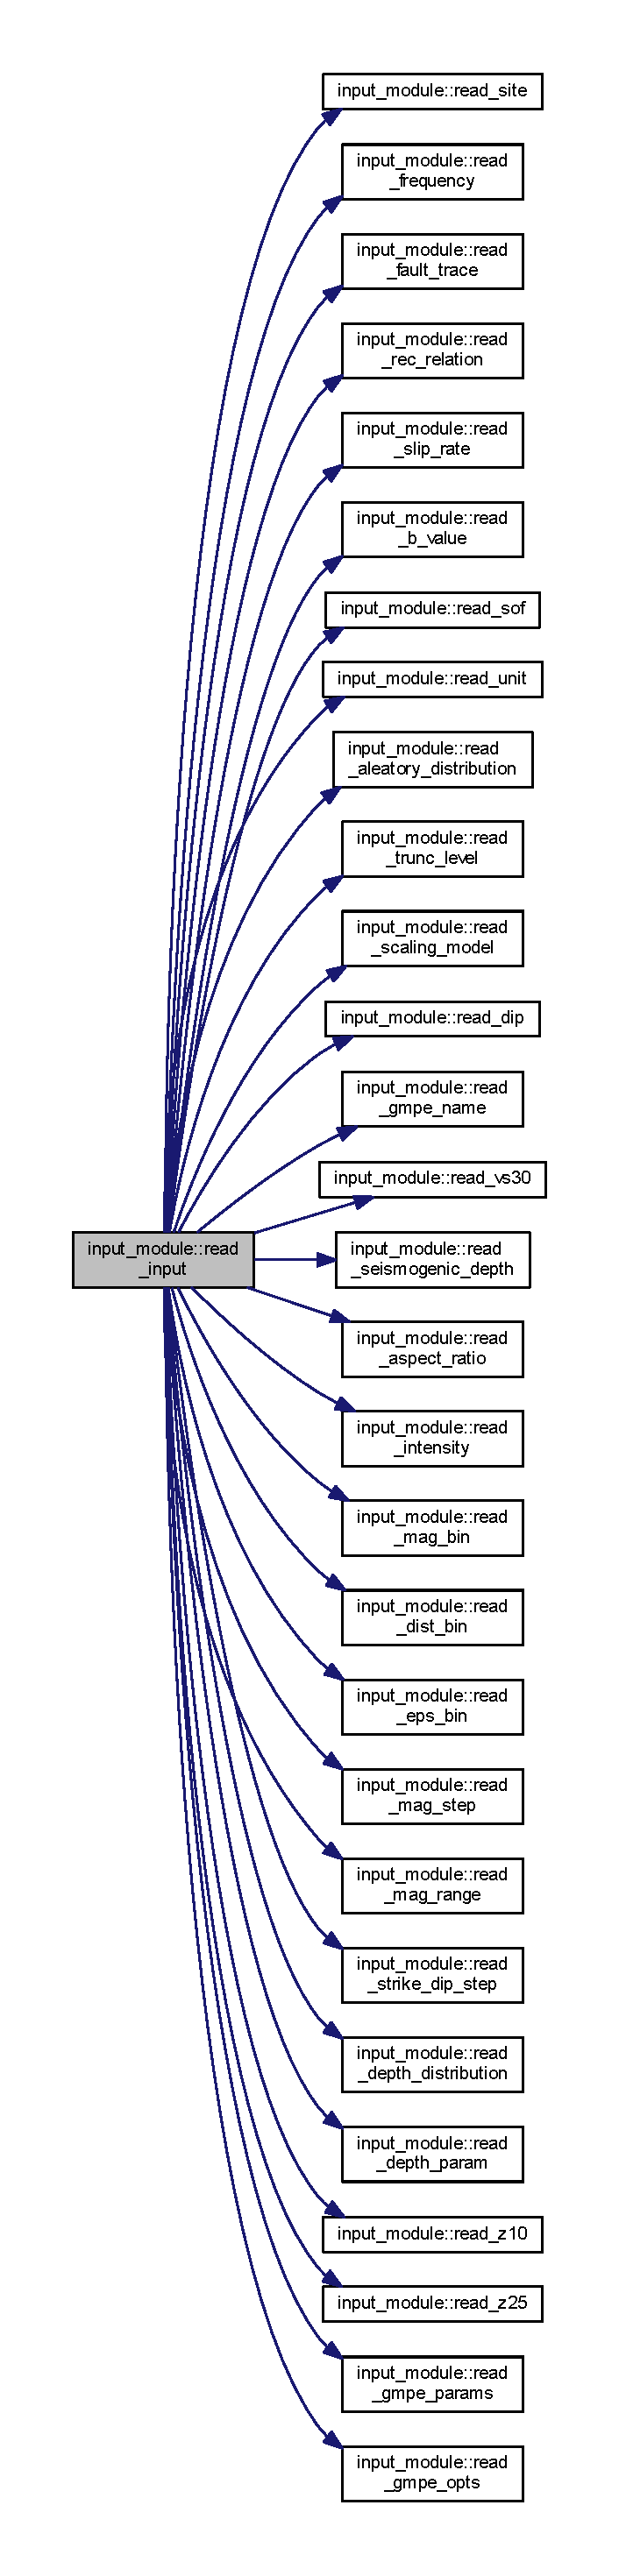
\includegraphics[height=550pt]{namespaceinput__module_a00c4a5d066f42d27b85b05a38bed5160_cgraph}
\end{center}
\end{figure}


\hypertarget{namespaceinput__module_acd40b5b88af0a4f619e2054305e670bb}{}\index{input\+\_\+module@{input\+\_\+module}!read\+\_\+intensity@{read\+\_\+intensity}}
\index{read\+\_\+intensity@{read\+\_\+intensity}!input\+\_\+module@{input\+\_\+module}}
\subsubsection[{read\+\_\+intensity()}]{\setlength{\rightskip}{0pt plus 5cm}subroutine input\+\_\+module\+::read\+\_\+intensity (
\begin{DoxyParamCaption}
{}
\end{DoxyParamCaption}
)}\label{namespaceinput__module_acd40b5b88af0a4f619e2054305e670bb}
\hypertarget{namespaceinput__module_a9cf8432b15120af2d78057266ef67ae0}{}\index{input\+\_\+module@{input\+\_\+module}!read\+\_\+mag\+\_\+bin@{read\+\_\+mag\+\_\+bin}}
\index{read\+\_\+mag\+\_\+bin@{read\+\_\+mag\+\_\+bin}!input\+\_\+module@{input\+\_\+module}}
\subsubsection[{read\+\_\+mag\+\_\+bin()}]{\setlength{\rightskip}{0pt plus 5cm}subroutine input\+\_\+module\+::read\+\_\+mag\+\_\+bin (
\begin{DoxyParamCaption}
{}
\end{DoxyParamCaption}
)}\label{namespaceinput__module_a9cf8432b15120af2d78057266ef67ae0}
\hypertarget{namespaceinput__module_a9277ed03dfb00814405f98a5b0455d1c}{}\index{input\+\_\+module@{input\+\_\+module}!read\+\_\+mag\+\_\+range@{read\+\_\+mag\+\_\+range}}
\index{read\+\_\+mag\+\_\+range@{read\+\_\+mag\+\_\+range}!input\+\_\+module@{input\+\_\+module}}
\subsubsection[{read\+\_\+mag\+\_\+range()}]{\setlength{\rightskip}{0pt plus 5cm}subroutine input\+\_\+module\+::read\+\_\+mag\+\_\+range (
\begin{DoxyParamCaption}
{}
\end{DoxyParamCaption}
)}\label{namespaceinput__module_a9277ed03dfb00814405f98a5b0455d1c}
\hypertarget{namespaceinput__module_a236da7bc51e5b4d79ef626a76b8dbea1}{}\index{input\+\_\+module@{input\+\_\+module}!read\+\_\+mag\+\_\+step@{read\+\_\+mag\+\_\+step}}
\index{read\+\_\+mag\+\_\+step@{read\+\_\+mag\+\_\+step}!input\+\_\+module@{input\+\_\+module}}
\subsubsection[{read\+\_\+mag\+\_\+step()}]{\setlength{\rightskip}{0pt plus 5cm}subroutine input\+\_\+module\+::read\+\_\+mag\+\_\+step (
\begin{DoxyParamCaption}
{}
\end{DoxyParamCaption}
)}\label{namespaceinput__module_a236da7bc51e5b4d79ef626a76b8dbea1}
\hypertarget{namespaceinput__module_a1e706b509f806cf51ec52d88f6be16f5}{}\index{input\+\_\+module@{input\+\_\+module}!read\+\_\+rec\+\_\+relation@{read\+\_\+rec\+\_\+relation}}
\index{read\+\_\+rec\+\_\+relation@{read\+\_\+rec\+\_\+relation}!input\+\_\+module@{input\+\_\+module}}
\subsubsection[{read\+\_\+rec\+\_\+relation()}]{\setlength{\rightskip}{0pt plus 5cm}subroutine input\+\_\+module\+::read\+\_\+rec\+\_\+relation (
\begin{DoxyParamCaption}
{}
\end{DoxyParamCaption}
)}\label{namespaceinput__module_a1e706b509f806cf51ec52d88f6be16f5}
\hypertarget{namespaceinput__module_a0c45a351fde1aa9a3fe8f15c1d78330e}{}\index{input\+\_\+module@{input\+\_\+module}!read\+\_\+scaling\+\_\+model@{read\+\_\+scaling\+\_\+model}}
\index{read\+\_\+scaling\+\_\+model@{read\+\_\+scaling\+\_\+model}!input\+\_\+module@{input\+\_\+module}}
\subsubsection[{read\+\_\+scaling\+\_\+model}]{\setlength{\rightskip}{0pt plus 5cm}subroutine input\+\_\+module\+::read\+\_\+scaling\+\_\+model (
\begin{DoxyParamCaption}
{}
\end{DoxyParamCaption}
)}\label{namespaceinput__module_a0c45a351fde1aa9a3fe8f15c1d78330e}
\hypertarget{namespaceinput__module_a3b50bd9377741e86fbc4f43ec8e5ef93}{}\index{input\+\_\+module@{input\+\_\+module}!read\+\_\+seismogenic\+\_\+depth@{read\+\_\+seismogenic\+\_\+depth}}
\index{read\+\_\+seismogenic\+\_\+depth@{read\+\_\+seismogenic\+\_\+depth}!input\+\_\+module@{input\+\_\+module}}
\subsubsection[{read\+\_\+seismogenic\+\_\+depth()}]{\setlength{\rightskip}{0pt plus 5cm}subroutine input\+\_\+module\+::read\+\_\+seismogenic\+\_\+depth (
\begin{DoxyParamCaption}
{}
\end{DoxyParamCaption}
)}\label{namespaceinput__module_a3b50bd9377741e86fbc4f43ec8e5ef93}
\hypertarget{namespaceinput__module_a07cd15a61e7f02633605f2f442ceb937}{}\index{input\+\_\+module@{input\+\_\+module}!read\+\_\+site@{read\+\_\+site}}
\index{read\+\_\+site@{read\+\_\+site}!input\+\_\+module@{input\+\_\+module}}
\subsubsection[{read\+\_\+site()}]{\setlength{\rightskip}{0pt plus 5cm}subroutine input\+\_\+module\+::read\+\_\+site (
\begin{DoxyParamCaption}
{}
\end{DoxyParamCaption}
)}\label{namespaceinput__module_a07cd15a61e7f02633605f2f442ceb937}
\hypertarget{namespaceinput__module_a162c082b34aa3c082906be0b3260e07b}{}\index{input\+\_\+module@{input\+\_\+module}!read\+\_\+slip\+\_\+rate@{read\+\_\+slip\+\_\+rate}}
\index{read\+\_\+slip\+\_\+rate@{read\+\_\+slip\+\_\+rate}!input\+\_\+module@{input\+\_\+module}}
\subsubsection[{read\+\_\+slip\+\_\+rate()}]{\setlength{\rightskip}{0pt plus 5cm}subroutine input\+\_\+module\+::read\+\_\+slip\+\_\+rate (
\begin{DoxyParamCaption}
{}
\end{DoxyParamCaption}
)}\label{namespaceinput__module_a162c082b34aa3c082906be0b3260e07b}
\hypertarget{namespaceinput__module_acc844c5a0060bf20c9ae19ac3d2e3740}{}\index{input\+\_\+module@{input\+\_\+module}!read\+\_\+sof@{read\+\_\+sof}}
\index{read\+\_\+sof@{read\+\_\+sof}!input\+\_\+module@{input\+\_\+module}}
\subsubsection[{read\+\_\+sof()}]{\setlength{\rightskip}{0pt plus 5cm}subroutine input\+\_\+module\+::read\+\_\+sof (
\begin{DoxyParamCaption}
{}
\end{DoxyParamCaption}
)}\label{namespaceinput__module_acc844c5a0060bf20c9ae19ac3d2e3740}
\hypertarget{namespaceinput__module_a82104204d5b1aff59b087d4b87cf166b}{}\index{input\+\_\+module@{input\+\_\+module}!read\+\_\+strike\+\_\+dip\+\_\+step@{read\+\_\+strike\+\_\+dip\+\_\+step}}
\index{read\+\_\+strike\+\_\+dip\+\_\+step@{read\+\_\+strike\+\_\+dip\+\_\+step}!input\+\_\+module@{input\+\_\+module}}
\subsubsection[{read\+\_\+strike\+\_\+dip\+\_\+step()}]{\setlength{\rightskip}{0pt plus 5cm}subroutine input\+\_\+module\+::read\+\_\+strike\+\_\+dip\+\_\+step (
\begin{DoxyParamCaption}
{}
\end{DoxyParamCaption}
)}\label{namespaceinput__module_a82104204d5b1aff59b087d4b87cf166b}
\hypertarget{namespaceinput__module_a57f855a995185ff6d52c0a402a4a536b}{}\index{input\+\_\+module@{input\+\_\+module}!read\+\_\+trunc\+\_\+level@{read\+\_\+trunc\+\_\+level}}
\index{read\+\_\+trunc\+\_\+level@{read\+\_\+trunc\+\_\+level}!input\+\_\+module@{input\+\_\+module}}
\subsubsection[{read\+\_\+trunc\+\_\+level()}]{\setlength{\rightskip}{0pt plus 5cm}subroutine input\+\_\+module\+::read\+\_\+trunc\+\_\+level (
\begin{DoxyParamCaption}
{}
\end{DoxyParamCaption}
)}\label{namespaceinput__module_a57f855a995185ff6d52c0a402a4a536b}
\hypertarget{namespaceinput__module_af0a24a3c1c27d7891b4ca97e8cbf73e8}{}\index{input\+\_\+module@{input\+\_\+module}!read\+\_\+unit@{read\+\_\+unit}}
\index{read\+\_\+unit@{read\+\_\+unit}!input\+\_\+module@{input\+\_\+module}}
\subsubsection[{read\+\_\+unit()}]{\setlength{\rightskip}{0pt plus 5cm}subroutine input\+\_\+module\+::read\+\_\+unit (
\begin{DoxyParamCaption}
{}
\end{DoxyParamCaption}
)}\label{namespaceinput__module_af0a24a3c1c27d7891b4ca97e8cbf73e8}
\hypertarget{namespaceinput__module_a4989c6ca8bc90648ca9587bee66d26b1}{}\index{input\+\_\+module@{input\+\_\+module}!read\+\_\+vs30@{read\+\_\+vs30}}
\index{read\+\_\+vs30@{read\+\_\+vs30}!input\+\_\+module@{input\+\_\+module}}
\subsubsection[{read\+\_\+vs30()}]{\setlength{\rightskip}{0pt plus 5cm}subroutine input\+\_\+module\+::read\+\_\+vs30 (
\begin{DoxyParamCaption}
{}
\end{DoxyParamCaption}
)}\label{namespaceinput__module_a4989c6ca8bc90648ca9587bee66d26b1}
\hypertarget{namespaceinput__module_a79ff648d45e7ac3f88ed461464c23901}{}\index{input\+\_\+module@{input\+\_\+module}!read\+\_\+z10@{read\+\_\+z10}}
\index{read\+\_\+z10@{read\+\_\+z10}!input\+\_\+module@{input\+\_\+module}}
\subsubsection[{read\+\_\+z10()}]{\setlength{\rightskip}{0pt plus 5cm}subroutine input\+\_\+module\+::read\+\_\+z10 (
\begin{DoxyParamCaption}
{}
\end{DoxyParamCaption}
)}\label{namespaceinput__module_a79ff648d45e7ac3f88ed461464c23901}
\hypertarget{namespaceinput__module_a37d4fe4627c2f2d2f7063f9df9730476}{}\index{input\+\_\+module@{input\+\_\+module}!read\+\_\+z25@{read\+\_\+z25}}
\index{read\+\_\+z25@{read\+\_\+z25}!input\+\_\+module@{input\+\_\+module}}
\subsubsection[{read\+\_\+z25()}]{\setlength{\rightskip}{0pt plus 5cm}subroutine input\+\_\+module\+::read\+\_\+z25 (
\begin{DoxyParamCaption}
{}
\end{DoxyParamCaption}
)}\label{namespaceinput__module_a37d4fe4627c2f2d2f7063f9df9730476}


\subsection{Variable Documentation}
\hypertarget{namespaceinput__module_a7f573d3c228f74f193a801e6cb1175ef}{}\index{input\+\_\+module@{input\+\_\+module}!arg@{arg}}
\index{arg@{arg}!input\+\_\+module@{input\+\_\+module}}
\subsubsection[{arg}]{\setlength{\rightskip}{0pt plus 5cm}character(130) input\+\_\+module\+::arg}\label{namespaceinput__module_a7f573d3c228f74f193a801e6cb1175ef}
\hypertarget{namespaceinput__module_ab4d6a4549b55a71a3451143893707ad2}{}\index{input\+\_\+module@{input\+\_\+module}!aspect\+\_\+ratio@{aspect\+\_\+ratio}}
\index{aspect\+\_\+ratio@{aspect\+\_\+ratio}!input\+\_\+module@{input\+\_\+module}}
\subsubsection[{aspect\+\_\+ratio}]{\setlength{\rightskip}{0pt plus 5cm}real(8) input\+\_\+module\+::aspect\+\_\+ratio}\label{namespaceinput__module_ab4d6a4549b55a71a3451143893707ad2}
\hypertarget{namespaceinput__module_a44ab6716b820721bceea32b98883fcdd}{}\index{input\+\_\+module@{input\+\_\+module}!b\+\_\+value@{b\+\_\+value}}
\index{b\+\_\+value@{b\+\_\+value}!input\+\_\+module@{input\+\_\+module}}
\subsubsection[{b\+\_\+value}]{\setlength{\rightskip}{0pt plus 5cm}real(8) input\+\_\+module\+::b\+\_\+value}\label{namespaceinput__module_a44ab6716b820721bceea32b98883fcdd}
\hypertarget{namespaceinput__module_af24dc133394110c4b8722a650aa7aab5}{}\index{input\+\_\+module@{input\+\_\+module}!depth\+\_\+param@{depth\+\_\+param}}
\index{depth\+\_\+param@{depth\+\_\+param}!input\+\_\+module@{input\+\_\+module}}
\subsubsection[{depth\+\_\+param}]{\setlength{\rightskip}{0pt plus 5cm}real(8) input\+\_\+module\+::depth\+\_\+param}\label{namespaceinput__module_af24dc133394110c4b8722a650aa7aab5}
\hypertarget{namespaceinput__module_a88d165b66edaf4e0dc9efbc76d5334b3}{}\index{input\+\_\+module@{input\+\_\+module}!dip\+\_\+step@{dip\+\_\+step}}
\index{dip\+\_\+step@{dip\+\_\+step}!input\+\_\+module@{input\+\_\+module}}
\subsubsection[{dip\+\_\+step}]{\setlength{\rightskip}{0pt plus 5cm}real(8) input\+\_\+module\+::dip\+\_\+step}\label{namespaceinput__module_a88d165b66edaf4e0dc9efbc76d5334b3}
\hypertarget{namespaceinput__module_a760ea371c13a02c658f3ec689a63adad}{}\index{input\+\_\+module@{input\+\_\+module}!dist\+\_\+bin@{dist\+\_\+bin}}
\index{dist\+\_\+bin@{dist\+\_\+bin}!input\+\_\+module@{input\+\_\+module}}
\subsubsection[{dist\+\_\+bin}]{\setlength{\rightskip}{0pt plus 5cm}real(8), dimension(\+:), allocatable input\+\_\+module\+::dist\+\_\+bin}\label{namespaceinput__module_a760ea371c13a02c658f3ec689a63adad}
\hypertarget{namespaceinput__module_ada333752feb1551085c3d0331da41a6d}{}\index{input\+\_\+module@{input\+\_\+module}!eastat@{eastat}}
\index{eastat@{eastat}!input\+\_\+module@{input\+\_\+module}}
\subsubsection[{eastat}]{\setlength{\rightskip}{0pt plus 5cm}integer input\+\_\+module\+::eastat}\label{namespaceinput__module_ada333752feb1551085c3d0331da41a6d}
\hypertarget{namespaceinput__module_a6900d0ebf1a2f906895db37f5b82e495}{}\index{input\+\_\+module@{input\+\_\+module}!eps\+\_\+bin@{eps\+\_\+bin}}
\index{eps\+\_\+bin@{eps\+\_\+bin}!input\+\_\+module@{input\+\_\+module}}
\subsubsection[{eps\+\_\+bin}]{\setlength{\rightskip}{0pt plus 5cm}real(8), dimension(\+:), allocatable input\+\_\+module\+::eps\+\_\+bin}\label{namespaceinput__module_a6900d0ebf1a2f906895db37f5b82e495}
\hypertarget{namespaceinput__module_ab8a4b6a5af6ac707c4c8656e4d709bec}{}\index{input\+\_\+module@{input\+\_\+module}!ext\+\_\+dag@{ext\+\_\+dag}}
\index{ext\+\_\+dag@{ext\+\_\+dag}!input\+\_\+module@{input\+\_\+module}}
\subsubsection[{ext\+\_\+dag}]{\setlength{\rightskip}{0pt plus 5cm}character(3) input\+\_\+module\+::ext\+\_\+dag = \textquotesingle{}dag\textquotesingle{}}\label{namespaceinput__module_ab8a4b6a5af6ac707c4c8656e4d709bec}
\hypertarget{namespaceinput__module_a860f66b4ca95c52a45651e1a7033e302}{}\index{input\+\_\+module@{input\+\_\+module}!ext\+\_\+haz@{ext\+\_\+haz}}
\index{ext\+\_\+haz@{ext\+\_\+haz}!input\+\_\+module@{input\+\_\+module}}
\subsubsection[{ext\+\_\+haz}]{\setlength{\rightskip}{0pt plus 5cm}character(3) input\+\_\+module\+::ext\+\_\+haz = \textquotesingle{}haz\textquotesingle{}}\label{namespaceinput__module_a860f66b4ca95c52a45651e1a7033e302}
\hypertarget{namespaceinput__module_a781c43885db3614608686197e48ab56b}{}\index{input\+\_\+module@{input\+\_\+module}!ext\+\_\+log@{ext\+\_\+log}}
\index{ext\+\_\+log@{ext\+\_\+log}!input\+\_\+module@{input\+\_\+module}}
\subsubsection[{ext\+\_\+log}]{\setlength{\rightskip}{0pt plus 5cm}character(3) input\+\_\+module\+::ext\+\_\+log = \textquotesingle{}log\textquotesingle{}}\label{namespaceinput__module_a781c43885db3614608686197e48ab56b}
\hypertarget{namespaceinput__module_a5ba0c6f56b537efe7105ffc5ef3a9a98}{}\index{input\+\_\+module@{input\+\_\+module}!ext\+\_\+rup@{ext\+\_\+rup}}
\index{ext\+\_\+rup@{ext\+\_\+rup}!input\+\_\+module@{input\+\_\+module}}
\subsubsection[{ext\+\_\+rup}]{\setlength{\rightskip}{0pt plus 5cm}character(3) input\+\_\+module\+::ext\+\_\+rup = \textquotesingle{}rup\textquotesingle{}}\label{namespaceinput__module_a5ba0c6f56b537efe7105ffc5ef3a9a98}
\hypertarget{namespaceinput__module_aab1c202e5a9b8804c86cf645932291d6}{}\index{input\+\_\+module@{input\+\_\+module}!flt\+\_\+dip\+\_\+deg@{flt\+\_\+dip\+\_\+deg}}
\index{flt\+\_\+dip\+\_\+deg@{flt\+\_\+dip\+\_\+deg}!input\+\_\+module@{input\+\_\+module}}
\subsubsection[{flt\+\_\+dip\+\_\+deg}]{\setlength{\rightskip}{0pt plus 5cm}real(8) input\+\_\+module\+::flt\+\_\+dip\+\_\+deg}\label{namespaceinput__module_aab1c202e5a9b8804c86cf645932291d6}
\hypertarget{namespaceinput__module_a00a633afb5b4d59fbb59372da1b72dd5}{}\index{input\+\_\+module@{input\+\_\+module}!flt\+\_\+dip\+\_\+rad@{flt\+\_\+dip\+\_\+rad}}
\index{flt\+\_\+dip\+\_\+rad@{flt\+\_\+dip\+\_\+rad}!input\+\_\+module@{input\+\_\+module}}
\subsubsection[{flt\+\_\+dip\+\_\+rad}]{\setlength{\rightskip}{0pt plus 5cm}real(8) input\+\_\+module\+::flt\+\_\+dip\+\_\+rad}\label{namespaceinput__module_a00a633afb5b4d59fbb59372da1b72dd5}
\hypertarget{namespaceinput__module_ab43a73209bacb0daeff92dd8758952b6}{}\index{input\+\_\+module@{input\+\_\+module}!flt\+\_\+n\+\_\+corner@{flt\+\_\+n\+\_\+corner}}
\index{flt\+\_\+n\+\_\+corner@{flt\+\_\+n\+\_\+corner}!input\+\_\+module@{input\+\_\+module}}
\subsubsection[{flt\+\_\+n\+\_\+corner}]{\setlength{\rightskip}{0pt plus 5cm}integer input\+\_\+module\+::flt\+\_\+n\+\_\+corner}\label{namespaceinput__module_ab43a73209bacb0daeff92dd8758952b6}
\hypertarget{namespaceinput__module_ab8cf9e7e4661e076527f292296cca198}{}\index{input\+\_\+module@{input\+\_\+module}!flt\+\_\+n\+\_\+seg@{flt\+\_\+n\+\_\+seg}}
\index{flt\+\_\+n\+\_\+seg@{flt\+\_\+n\+\_\+seg}!input\+\_\+module@{input\+\_\+module}}
\subsubsection[{flt\+\_\+n\+\_\+seg}]{\setlength{\rightskip}{0pt plus 5cm}integer input\+\_\+module\+::flt\+\_\+n\+\_\+seg}\label{namespaceinput__module_ab8cf9e7e4661e076527f292296cca198}
\hypertarget{namespaceinput__module_a289e412144c4ad26f482d664135f3972}{}\index{input\+\_\+module@{input\+\_\+module}!flt\+\_\+trace@{flt\+\_\+trace}}
\index{flt\+\_\+trace@{flt\+\_\+trace}!input\+\_\+module@{input\+\_\+module}}
\subsubsection[{flt\+\_\+trace}]{\setlength{\rightskip}{0pt plus 5cm}real(8), dimension(\+:,\+:), allocatable input\+\_\+module\+::flt\+\_\+trace}\label{namespaceinput__module_a289e412144c4ad26f482d664135f3972}
\hypertarget{namespaceinput__module_ae99c24908c83beaac79f68a46d079e37}{}\index{input\+\_\+module@{input\+\_\+module}!fnm\+\_\+dag@{fnm\+\_\+dag}}
\index{fnm\+\_\+dag@{fnm\+\_\+dag}!input\+\_\+module@{input\+\_\+module}}
\subsubsection[{fnm\+\_\+dag}]{\setlength{\rightskip}{0pt plus 5cm}character(130) input\+\_\+module\+::fnm\+\_\+dag}\label{namespaceinput__module_ae99c24908c83beaac79f68a46d079e37}
\hypertarget{namespaceinput__module_ab37b626c8a9c8a0ad42d001c9a0e5ac4}{}\index{input\+\_\+module@{input\+\_\+module}!fnm\+\_\+haz@{fnm\+\_\+haz}}
\index{fnm\+\_\+haz@{fnm\+\_\+haz}!input\+\_\+module@{input\+\_\+module}}
\subsubsection[{fnm\+\_\+haz}]{\setlength{\rightskip}{0pt plus 5cm}character(130) input\+\_\+module\+::fnm\+\_\+haz}\label{namespaceinput__module_ab37b626c8a9c8a0ad42d001c9a0e5ac4}
\hypertarget{namespaceinput__module_ad228ac099c1afd318803f2d8514dd2c9}{}\index{input\+\_\+module@{input\+\_\+module}!fnm\+\_\+inp@{fnm\+\_\+inp}}
\index{fnm\+\_\+inp@{fnm\+\_\+inp}!input\+\_\+module@{input\+\_\+module}}
\subsubsection[{fnm\+\_\+inp}]{\setlength{\rightskip}{0pt plus 5cm}character(130) input\+\_\+module\+::fnm\+\_\+inp}\label{namespaceinput__module_ad228ac099c1afd318803f2d8514dd2c9}
\hypertarget{namespaceinput__module_a95df80960079d35b95016b2448da8dcc}{}\index{input\+\_\+module@{input\+\_\+module}!fnm\+\_\+log@{fnm\+\_\+log}}
\index{fnm\+\_\+log@{fnm\+\_\+log}!input\+\_\+module@{input\+\_\+module}}
\subsubsection[{fnm\+\_\+log}]{\setlength{\rightskip}{0pt plus 5cm}character(130) input\+\_\+module\+::fnm\+\_\+log}\label{namespaceinput__module_a95df80960079d35b95016b2448da8dcc}
\hypertarget{namespaceinput__module_a913978d3f2a95df35b24c099c6599cd0}{}\index{input\+\_\+module@{input\+\_\+module}!fnm\+\_\+rup@{fnm\+\_\+rup}}
\index{fnm\+\_\+rup@{fnm\+\_\+rup}!input\+\_\+module@{input\+\_\+module}}
\subsubsection[{fnm\+\_\+rup}]{\setlength{\rightskip}{0pt plus 5cm}character(130) input\+\_\+module\+::fnm\+\_\+rup}\label{namespaceinput__module_a913978d3f2a95df35b24c099c6599cd0}
\hypertarget{namespaceinput__module_a52ffef6eb6299a12612cc0b2eb5352dc}{}\index{input\+\_\+module@{input\+\_\+module}!fp\+\_\+dag@{fp\+\_\+dag}}
\index{fp\+\_\+dag@{fp\+\_\+dag}!input\+\_\+module@{input\+\_\+module}}
\subsubsection[{fp\+\_\+dag}]{\setlength{\rightskip}{0pt plus 5cm}integer input\+\_\+module\+::fp\+\_\+dag}\label{namespaceinput__module_a52ffef6eb6299a12612cc0b2eb5352dc}
\hypertarget{namespaceinput__module_a5b74d4c157160f6d6eaef2c725b02d6a}{}\index{input\+\_\+module@{input\+\_\+module}!fp\+\_\+haz@{fp\+\_\+haz}}
\index{fp\+\_\+haz@{fp\+\_\+haz}!input\+\_\+module@{input\+\_\+module}}
\subsubsection[{fp\+\_\+haz}]{\setlength{\rightskip}{0pt plus 5cm}integer input\+\_\+module\+::fp\+\_\+haz}\label{namespaceinput__module_a5b74d4c157160f6d6eaef2c725b02d6a}
\hypertarget{namespaceinput__module_a7d1f1dd6198e0770d9218a80115df0de}{}\index{input\+\_\+module@{input\+\_\+module}!fp\+\_\+inp@{fp\+\_\+inp}}
\index{fp\+\_\+inp@{fp\+\_\+inp}!input\+\_\+module@{input\+\_\+module}}
\subsubsection[{fp\+\_\+inp}]{\setlength{\rightskip}{0pt plus 5cm}integer input\+\_\+module\+::fp\+\_\+inp}\label{namespaceinput__module_a7d1f1dd6198e0770d9218a80115df0de}
\hypertarget{namespaceinput__module_a24121f5e413cdf763ada92cb0c916ba3}{}\index{input\+\_\+module@{input\+\_\+module}!fp\+\_\+log@{fp\+\_\+log}}
\index{fp\+\_\+log@{fp\+\_\+log}!input\+\_\+module@{input\+\_\+module}}
\subsubsection[{fp\+\_\+log}]{\setlength{\rightskip}{0pt plus 5cm}integer input\+\_\+module\+::fp\+\_\+log}\label{namespaceinput__module_a24121f5e413cdf763ada92cb0c916ba3}
\hypertarget{namespaceinput__module_a73158a89ce75123f19e014408bb9b342}{}\index{input\+\_\+module@{input\+\_\+module}!fp\+\_\+rup@{fp\+\_\+rup}}
\index{fp\+\_\+rup@{fp\+\_\+rup}!input\+\_\+module@{input\+\_\+module}}
\subsubsection[{fp\+\_\+rup}]{\setlength{\rightskip}{0pt plus 5cm}integer input\+\_\+module\+::fp\+\_\+rup}\label{namespaceinput__module_a73158a89ce75123f19e014408bb9b342}
\hypertarget{namespaceinput__module_a2eec881a49e9f9d341e49f123b8435a3}{}\index{input\+\_\+module@{input\+\_\+module}!frequency@{frequency}}
\index{frequency@{frequency}!input\+\_\+module@{input\+\_\+module}}
\subsubsection[{frequency}]{\setlength{\rightskip}{0pt plus 5cm}real(8), dimension(\+:), allocatable input\+\_\+module\+::frequency}\label{namespaceinput__module_a2eec881a49e9f9d341e49f123b8435a3}
\hypertarget{namespaceinput__module_ae241dcd6d1b9e390d39acb1f7ed2f38b}{}\index{input\+\_\+module@{input\+\_\+module}!gmpe\+\_\+name@{gmpe\+\_\+name}}
\index{gmpe\+\_\+name@{gmpe\+\_\+name}!input\+\_\+module@{input\+\_\+module}}
\subsubsection[{gmpe\+\_\+name}]{\setlength{\rightskip}{0pt plus 5cm}character(130) input\+\_\+module\+::gmpe\+\_\+name}\label{namespaceinput__module_ae241dcd6d1b9e390d39acb1f7ed2f38b}
\hypertarget{namespaceinput__module_a1c956fb0e5942428da3bdb0c932fd10c}{}\index{input\+\_\+module@{input\+\_\+module}!gmpe\+\_\+opts@{gmpe\+\_\+opts}}
\index{gmpe\+\_\+opts@{gmpe\+\_\+opts}!input\+\_\+module@{input\+\_\+module}}
\subsubsection[{gmpe\+\_\+opts}]{\setlength{\rightskip}{0pt plus 5cm}integer, dimension(\+:), allocatable input\+\_\+module\+::gmpe\+\_\+opts}\label{namespaceinput__module_a1c956fb0e5942428da3bdb0c932fd10c}
\hypertarget{namespaceinput__module_ab52a267c1d75b879ad598fa6cc377c4b}{}\index{input\+\_\+module@{input\+\_\+module}!gmpe\+\_\+params@{gmpe\+\_\+params}}
\index{gmpe\+\_\+params@{gmpe\+\_\+params}!input\+\_\+module@{input\+\_\+module}}
\subsubsection[{gmpe\+\_\+params}]{\setlength{\rightskip}{0pt plus 5cm}real(8), dimension(\+:), allocatable input\+\_\+module\+::gmpe\+\_\+params}\label{namespaceinput__module_ab52a267c1d75b879ad598fa6cc377c4b}
\hypertarget{namespaceinput__module_af09923ed6808263d4497c13126abdb46}{}\index{input\+\_\+module@{input\+\_\+module}!inp\+\_\+exist@{inp\+\_\+exist}}
\index{inp\+\_\+exist@{inp\+\_\+exist}!input\+\_\+module@{input\+\_\+module}}
\subsubsection[{inp\+\_\+exist}]{\setlength{\rightskip}{0pt plus 5cm}logical input\+\_\+module\+::inp\+\_\+exist}\label{namespaceinput__module_af09923ed6808263d4497c13126abdb46}
\hypertarget{namespaceinput__module_ab8a5b4989aa8a656c28df7fa39f21d03}{}\index{input\+\_\+module@{input\+\_\+module}!intensity@{intensity}}
\index{intensity@{intensity}!input\+\_\+module@{input\+\_\+module}}
\subsubsection[{intensity}]{\setlength{\rightskip}{0pt plus 5cm}real(8), dimension(\+:), allocatable input\+\_\+module\+::intensity}\label{namespaceinput__module_ab8a5b4989aa8a656c28df7fa39f21d03}
\hypertarget{namespaceinput__module_a865cd5e2924fbc40aeefe8bcb6226a75}{}\index{input\+\_\+module@{input\+\_\+module}!iost@{iost}}
\index{iost@{iost}!input\+\_\+module@{input\+\_\+module}}
\subsubsection[{iost}]{\setlength{\rightskip}{0pt plus 5cm}integer input\+\_\+module\+::iost}\label{namespaceinput__module_a865cd5e2924fbc40aeefe8bcb6226a75}
\hypertarget{namespaceinput__module_a304ebe11a9b47adcaeb6db5be6bae12d}{}\index{input\+\_\+module@{input\+\_\+module}!line@{line}}
\index{line@{line}!input\+\_\+module@{input\+\_\+module}}
\subsubsection[{line}]{\setlength{\rightskip}{0pt plus 5cm}character(130) input\+\_\+module\+::line}\label{namespaceinput__module_a304ebe11a9b47adcaeb6db5be6bae12d}
\hypertarget{namespaceinput__module_a39c97f997959a940d039403c89a2b62c}{}\index{input\+\_\+module@{input\+\_\+module}!m\+\_\+aleatory\+\_\+distribution@{m\+\_\+aleatory\+\_\+distribution}}
\index{m\+\_\+aleatory\+\_\+distribution@{m\+\_\+aleatory\+\_\+distribution}!input\+\_\+module@{input\+\_\+module}}
\subsubsection[{m\+\_\+aleatory\+\_\+distribution}]{\setlength{\rightskip}{0pt plus 5cm}integer input\+\_\+module\+::m\+\_\+aleatory\+\_\+distribution}\label{namespaceinput__module_a39c97f997959a940d039403c89a2b62c}
\hypertarget{namespaceinput__module_acf6263946873708989398bfd2f91bbef}{}\index{input\+\_\+module@{input\+\_\+module}!m\+\_\+depth\+\_\+distribution@{m\+\_\+depth\+\_\+distribution}}
\index{m\+\_\+depth\+\_\+distribution@{m\+\_\+depth\+\_\+distribution}!input\+\_\+module@{input\+\_\+module}}
\subsubsection[{m\+\_\+depth\+\_\+distribution}]{\setlength{\rightskip}{0pt plus 5cm}integer input\+\_\+module\+::m\+\_\+depth\+\_\+distribution}\label{namespaceinput__module_acf6263946873708989398bfd2f91bbef}
\hypertarget{namespaceinput__module_a2426a45f38ebf777bbda4d215a04a11a}{}\index{input\+\_\+module@{input\+\_\+module}!m\+\_\+gmpe\+\_\+name@{m\+\_\+gmpe\+\_\+name}}
\index{m\+\_\+gmpe\+\_\+name@{m\+\_\+gmpe\+\_\+name}!input\+\_\+module@{input\+\_\+module}}
\subsubsection[{m\+\_\+gmpe\+\_\+name}]{\setlength{\rightskip}{0pt plus 5cm}integer input\+\_\+module\+::m\+\_\+gmpe\+\_\+name}\label{namespaceinput__module_a2426a45f38ebf777bbda4d215a04a11a}
\hypertarget{namespaceinput__module_acb06b69e7ed3cec59c693ab700ae7bc7}{}\index{input\+\_\+module@{input\+\_\+module}!m\+\_\+rec\+\_\+relation@{m\+\_\+rec\+\_\+relation}}
\index{m\+\_\+rec\+\_\+relation@{m\+\_\+rec\+\_\+relation}!input\+\_\+module@{input\+\_\+module}}
\subsubsection[{m\+\_\+rec\+\_\+relation}]{\setlength{\rightskip}{0pt plus 5cm}integer input\+\_\+module\+::m\+\_\+rec\+\_\+relation}\label{namespaceinput__module_acb06b69e7ed3cec59c693ab700ae7bc7}
\hypertarget{namespaceinput__module_ac8f94aead42fc3c3c63f6b80156c4392}{}\index{input\+\_\+module@{input\+\_\+module}!m\+\_\+scaling@{m\+\_\+scaling}}
\index{m\+\_\+scaling@{m\+\_\+scaling}!input\+\_\+module@{input\+\_\+module}}
\subsubsection[{m\+\_\+scaling}]{\setlength{\rightskip}{0pt plus 5cm}integer input\+\_\+module\+::m\+\_\+scaling}\label{namespaceinput__module_ac8f94aead42fc3c3c63f6b80156c4392}
\hypertarget{namespaceinput__module_a418d22665630502982d2925663df35cc}{}\index{input\+\_\+module@{input\+\_\+module}!m\+\_\+sigma\+\_\+trunc@{m\+\_\+sigma\+\_\+trunc}}
\index{m\+\_\+sigma\+\_\+trunc@{m\+\_\+sigma\+\_\+trunc}!input\+\_\+module@{input\+\_\+module}}
\subsubsection[{m\+\_\+sigma\+\_\+trunc}]{\setlength{\rightskip}{0pt plus 5cm}integer input\+\_\+module\+::m\+\_\+sigma\+\_\+trunc}\label{namespaceinput__module_a418d22665630502982d2925663df35cc}
\hypertarget{namespaceinput__module_afb3ee34150e00c5c18dddd5db73c0b9f}{}\index{input\+\_\+module@{input\+\_\+module}!m\+\_\+sof@{m\+\_\+sof}}
\index{m\+\_\+sof@{m\+\_\+sof}!input\+\_\+module@{input\+\_\+module}}
\subsubsection[{m\+\_\+sof}]{\setlength{\rightskip}{0pt plus 5cm}integer input\+\_\+module\+::m\+\_\+sof}\label{namespaceinput__module_afb3ee34150e00c5c18dddd5db73c0b9f}
\hypertarget{namespaceinput__module_a1a7790113ec65bfe00fa926b09b6a451}{}\index{input\+\_\+module@{input\+\_\+module}!m\+\_\+unit@{m\+\_\+unit}}
\index{m\+\_\+unit@{m\+\_\+unit}!input\+\_\+module@{input\+\_\+module}}
\subsubsection[{m\+\_\+unit}]{\setlength{\rightskip}{0pt plus 5cm}integer input\+\_\+module\+::m\+\_\+unit}\label{namespaceinput__module_a1a7790113ec65bfe00fa926b09b6a451}
\hypertarget{namespaceinput__module_a1bbdfb734d8c5f5b6370d1ab7fbfb04a}{}\index{input\+\_\+module@{input\+\_\+module}!mag\+\_\+bin@{mag\+\_\+bin}}
\index{mag\+\_\+bin@{mag\+\_\+bin}!input\+\_\+module@{input\+\_\+module}}
\subsubsection[{mag\+\_\+bin}]{\setlength{\rightskip}{0pt plus 5cm}real(8), dimension(\+:), allocatable input\+\_\+module\+::mag\+\_\+bin}\label{namespaceinput__module_a1bbdfb734d8c5f5b6370d1ab7fbfb04a}
\hypertarget{namespaceinput__module_a5f4a6ebb1c94126c9810b316e17976e2}{}\index{input\+\_\+module@{input\+\_\+module}!mag\+\_\+step@{mag\+\_\+step}}
\index{mag\+\_\+step@{mag\+\_\+step}!input\+\_\+module@{input\+\_\+module}}
\subsubsection[{mag\+\_\+step}]{\setlength{\rightskip}{0pt plus 5cm}real(8) input\+\_\+module\+::mag\+\_\+step}\label{namespaceinput__module_a5f4a6ebb1c94126c9810b316e17976e2}
\hypertarget{namespaceinput__module_a41ea519c5d8ed0def5faaee53d32171e}{}\index{input\+\_\+module@{input\+\_\+module}!mmax@{mmax}}
\index{mmax@{mmax}!input\+\_\+module@{input\+\_\+module}}
\subsubsection[{mmax}]{\setlength{\rightskip}{0pt plus 5cm}real(8) input\+\_\+module\+::mmax}\label{namespaceinput__module_a41ea519c5d8ed0def5faaee53d32171e}
\hypertarget{namespaceinput__module_a6f6194544ef970071393414d02104a8f}{}\index{input\+\_\+module@{input\+\_\+module}!mmin@{mmin}}
\index{mmin@{mmin}!input\+\_\+module@{input\+\_\+module}}
\subsubsection[{mmin}]{\setlength{\rightskip}{0pt plus 5cm}real(8) input\+\_\+module\+::mmin}\label{namespaceinput__module_a6f6194544ef970071393414d02104a8f}
\hypertarget{namespaceinput__module_ad9cff8fcf1650cc924462f2409ade59d}{}\index{input\+\_\+module@{input\+\_\+module}!n\+\_\+dist\+\_\+bin@{n\+\_\+dist\+\_\+bin}}
\index{n\+\_\+dist\+\_\+bin@{n\+\_\+dist\+\_\+bin}!input\+\_\+module@{input\+\_\+module}}
\subsubsection[{n\+\_\+dist\+\_\+bin}]{\setlength{\rightskip}{0pt plus 5cm}integer input\+\_\+module\+::n\+\_\+dist\+\_\+bin}\label{namespaceinput__module_ad9cff8fcf1650cc924462f2409ade59d}
\hypertarget{namespaceinput__module_a048d1cd2097b01c570f91e1166300c4d}{}\index{input\+\_\+module@{input\+\_\+module}!n\+\_\+eps\+\_\+bin@{n\+\_\+eps\+\_\+bin}}
\index{n\+\_\+eps\+\_\+bin@{n\+\_\+eps\+\_\+bin}!input\+\_\+module@{input\+\_\+module}}
\subsubsection[{n\+\_\+eps\+\_\+bin}]{\setlength{\rightskip}{0pt plus 5cm}integer input\+\_\+module\+::n\+\_\+eps\+\_\+bin}\label{namespaceinput__module_a048d1cd2097b01c570f91e1166300c4d}
\hypertarget{namespaceinput__module_a9c4337d8e000b4ec09cd937de3fec1a4}{}\index{input\+\_\+module@{input\+\_\+module}!n\+\_\+freq@{n\+\_\+freq}}
\index{n\+\_\+freq@{n\+\_\+freq}!input\+\_\+module@{input\+\_\+module}}
\subsubsection[{n\+\_\+freq}]{\setlength{\rightskip}{0pt plus 5cm}integer input\+\_\+module\+::n\+\_\+freq}\label{namespaceinput__module_a9c4337d8e000b4ec09cd937de3fec1a4}
\hypertarget{namespaceinput__module_a8e9793e0bad76077bc065ec13bc34910}{}\index{input\+\_\+module@{input\+\_\+module}!n\+\_\+inten@{n\+\_\+inten}}
\index{n\+\_\+inten@{n\+\_\+inten}!input\+\_\+module@{input\+\_\+module}}
\subsubsection[{n\+\_\+inten}]{\setlength{\rightskip}{0pt plus 5cm}integer input\+\_\+module\+::n\+\_\+inten}\label{namespaceinput__module_a8e9793e0bad76077bc065ec13bc34910}
\hypertarget{namespaceinput__module_a16e17c304087bd6dbbca884d691c3c6a}{}\index{input\+\_\+module@{input\+\_\+module}!n\+\_\+mag\+\_\+bin@{n\+\_\+mag\+\_\+bin}}
\index{n\+\_\+mag\+\_\+bin@{n\+\_\+mag\+\_\+bin}!input\+\_\+module@{input\+\_\+module}}
\subsubsection[{n\+\_\+mag\+\_\+bin}]{\setlength{\rightskip}{0pt plus 5cm}integer input\+\_\+module\+::n\+\_\+mag\+\_\+bin}\label{namespaceinput__module_a16e17c304087bd6dbbca884d691c3c6a}
\hypertarget{namespaceinput__module_ae55e8966862c5748b17a68539c94a6f6}{}\index{input\+\_\+module@{input\+\_\+module}!numvalues@{numvalues}}
\index{numvalues@{numvalues}!input\+\_\+module@{input\+\_\+module}}
\subsubsection[{numvalues}]{\setlength{\rightskip}{0pt plus 5cm}integer input\+\_\+module\+::numvalues}\label{namespaceinput__module_ae55e8966862c5748b17a68539c94a6f6}
\hypertarget{namespaceinput__module_a34271f9a9a4c0c0d531db4d9e2b05fc3}{}\index{input\+\_\+module@{input\+\_\+module}!ppos@{ppos}}
\index{ppos@{ppos}!input\+\_\+module@{input\+\_\+module}}
\subsubsection[{ppos}]{\setlength{\rightskip}{0pt plus 5cm}integer input\+\_\+module\+::ppos}\label{namespaceinput__module_a34271f9a9a4c0c0d531db4d9e2b05fc3}
\hypertarget{namespaceinput__module_ab574bddc682ceabd1271512c2b1f4e20}{}\index{input\+\_\+module@{input\+\_\+module}!site@{site}}
\index{site@{site}!input\+\_\+module@{input\+\_\+module}}
\subsubsection[{site}]{\setlength{\rightskip}{0pt plus 5cm}real(8), dimension(2) input\+\_\+module\+::site}\label{namespaceinput__module_ab574bddc682ceabd1271512c2b1f4e20}
\hypertarget{namespaceinput__module_a8c396f94a2d2aabe29bc5ba46c7c7fe0}{}\index{input\+\_\+module@{input\+\_\+module}!slip\+\_\+rate@{slip\+\_\+rate}}
\index{slip\+\_\+rate@{slip\+\_\+rate}!input\+\_\+module@{input\+\_\+module}}
\subsubsection[{slip\+\_\+rate}]{\setlength{\rightskip}{0pt plus 5cm}real(8) input\+\_\+module\+::slip\+\_\+rate}\label{namespaceinput__module_a8c396f94a2d2aabe29bc5ba46c7c7fe0}
\hypertarget{namespaceinput__module_a671a995c1135b6127af4ea5a418402ed}{}\index{input\+\_\+module@{input\+\_\+module}!smax@{smax}}
\index{smax@{smax}!input\+\_\+module@{input\+\_\+module}}
\subsubsection[{smax}]{\setlength{\rightskip}{0pt plus 5cm}real(8) input\+\_\+module\+::smax}\label{namespaceinput__module_a671a995c1135b6127af4ea5a418402ed}
\hypertarget{namespaceinput__module_a29a8cb54fcb208499fa3cf1b30131619}{}\index{input\+\_\+module@{input\+\_\+module}!smin@{smin}}
\index{smin@{smin}!input\+\_\+module@{input\+\_\+module}}
\subsubsection[{smin}]{\setlength{\rightskip}{0pt plus 5cm}real(8) input\+\_\+module\+::smin}\label{namespaceinput__module_a29a8cb54fcb208499fa3cf1b30131619}
\hypertarget{namespaceinput__module_aa2d7dcffb5650145aa835a858a0ad35a}{}\index{input\+\_\+module@{input\+\_\+module}!str\+\_\+tmp@{str\+\_\+tmp}}
\index{str\+\_\+tmp@{str\+\_\+tmp}!input\+\_\+module@{input\+\_\+module}}
\subsubsection[{str\+\_\+tmp}]{\setlength{\rightskip}{0pt plus 5cm}character(130) input\+\_\+module\+::str\+\_\+tmp}\label{namespaceinput__module_aa2d7dcffb5650145aa835a858a0ad35a}
\hypertarget{namespaceinput__module_aec362b5183a78823c9fd5604388f725e}{}\index{input\+\_\+module@{input\+\_\+module}!strike\+\_\+step@{strike\+\_\+step}}
\index{strike\+\_\+step@{strike\+\_\+step}!input\+\_\+module@{input\+\_\+module}}
\subsubsection[{strike\+\_\+step}]{\setlength{\rightskip}{0pt plus 5cm}real(8) input\+\_\+module\+::strike\+\_\+step}\label{namespaceinput__module_aec362b5183a78823c9fd5604388f725e}
\hypertarget{namespaceinput__module_a35e70ed5e2a0858cd4af8970e6b7a3fe}{}\index{input\+\_\+module@{input\+\_\+module}!temp1@{temp1}}
\index{temp1@{temp1}!input\+\_\+module@{input\+\_\+module}}
\subsubsection[{temp1}]{\setlength{\rightskip}{0pt plus 5cm}real(8), dimension(500) input\+\_\+module\+::temp1}\label{namespaceinput__module_a35e70ed5e2a0858cd4af8970e6b7a3fe}
\hypertarget{namespaceinput__module_ac72418d482bc6d9b164dc8ff77f80812}{}\index{input\+\_\+module@{input\+\_\+module}!temp2@{temp2}}
\index{temp2@{temp2}!input\+\_\+module@{input\+\_\+module}}
\subsubsection[{temp2}]{\setlength{\rightskip}{0pt plus 5cm}real(8), dimension(500,2) input\+\_\+module\+::temp2}\label{namespaceinput__module_ac72418d482bc6d9b164dc8ff77f80812}
\hypertarget{namespaceinput__module_a129d3471a7d48a92476195ec540b0599}{}\index{input\+\_\+module@{input\+\_\+module}!temp\+\_\+int@{temp\+\_\+int}}
\index{temp\+\_\+int@{temp\+\_\+int}!input\+\_\+module@{input\+\_\+module}}
\subsubsection[{temp\+\_\+int}]{\setlength{\rightskip}{0pt plus 5cm}integer, dimension(500) input\+\_\+module\+::temp\+\_\+int}\label{namespaceinput__module_a129d3471a7d48a92476195ec540b0599}
\hypertarget{namespaceinput__module_a1030c19aa6f6f484e8f538320aa753b0}{}\index{input\+\_\+module@{input\+\_\+module}!tmp1@{tmp1}}
\index{tmp1@{tmp1}!input\+\_\+module@{input\+\_\+module}}
\subsubsection[{tmp1}]{\setlength{\rightskip}{0pt plus 5cm}real(8) input\+\_\+module\+::tmp1}\label{namespaceinput__module_a1030c19aa6f6f484e8f538320aa753b0}
\hypertarget{namespaceinput__module_a4344e7e8b58aa6d6e534cc25168867dc}{}\index{input\+\_\+module@{input\+\_\+module}!tmp2@{tmp2}}
\index{tmp2@{tmp2}!input\+\_\+module@{input\+\_\+module}}
\subsubsection[{tmp2}]{\setlength{\rightskip}{0pt plus 5cm}real(8) input\+\_\+module\+::tmp2}\label{namespaceinput__module_a4344e7e8b58aa6d6e534cc25168867dc}
\hypertarget{namespaceinput__module_a98528ea542cc829033364307335ecdf6}{}\index{input\+\_\+module@{input\+\_\+module}!tmp\+\_\+int@{tmp\+\_\+int}}
\index{tmp\+\_\+int@{tmp\+\_\+int}!input\+\_\+module@{input\+\_\+module}}
\subsubsection[{tmp\+\_\+int}]{\setlength{\rightskip}{0pt plus 5cm}integer input\+\_\+module\+::tmp\+\_\+int}\label{namespaceinput__module_a98528ea542cc829033364307335ecdf6}
\hypertarget{namespaceinput__module_ae5dd4121bdb07e96089cd081a3017dd9}{}\index{input\+\_\+module@{input\+\_\+module}!trunc\+\_\+level@{trunc\+\_\+level}}
\index{trunc\+\_\+level@{trunc\+\_\+level}!input\+\_\+module@{input\+\_\+module}}
\subsubsection[{trunc\+\_\+level}]{\setlength{\rightskip}{0pt plus 5cm}real(8) input\+\_\+module\+::trunc\+\_\+level}\label{namespaceinput__module_ae5dd4121bdb07e96089cd081a3017dd9}
\hypertarget{namespaceinput__module_a1c64f18e0ac52016bea961845fd4f11e}{}\index{input\+\_\+module@{input\+\_\+module}!vs30@{vs30}}
\index{vs30@{vs30}!input\+\_\+module@{input\+\_\+module}}
\subsubsection[{vs30}]{\setlength{\rightskip}{0pt plus 5cm}real(8) input\+\_\+module\+::vs30}\label{namespaceinput__module_a1c64f18e0ac52016bea961845fd4f11e}
\hypertarget{namespaceinput__module_ae257590e746cae45e031d04017cf76d1}{}\index{input\+\_\+module@{input\+\_\+module}!wrt\+\_\+fmt@{wrt\+\_\+fmt}}
\index{wrt\+\_\+fmt@{wrt\+\_\+fmt}!input\+\_\+module@{input\+\_\+module}}
\subsubsection[{wrt\+\_\+fmt}]{\setlength{\rightskip}{0pt plus 5cm}character(130) input\+\_\+module\+::wrt\+\_\+fmt}\label{namespaceinput__module_ae257590e746cae45e031d04017cf76d1}
\hypertarget{namespaceinput__module_aa9efcd8b3636531d8be863c73c607ba7}{}\index{input\+\_\+module@{input\+\_\+module}!z10@{z10}}
\index{z10@{z10}!input\+\_\+module@{input\+\_\+module}}
\subsubsection[{z10}]{\setlength{\rightskip}{0pt plus 5cm}real(8) input\+\_\+module\+::z10}\label{namespaceinput__module_aa9efcd8b3636531d8be863c73c607ba7}
\hypertarget{namespaceinput__module_a397fb4f34e05ebd010c3a545e29b8eb3}{}\index{input\+\_\+module@{input\+\_\+module}!z25@{z25}}
\index{z25@{z25}!input\+\_\+module@{input\+\_\+module}}
\subsubsection[{z25}]{\setlength{\rightskip}{0pt plus 5cm}real(8) input\+\_\+module\+::z25}\label{namespaceinput__module_a397fb4f34e05ebd010c3a545e29b8eb3}

\hypertarget{namespaceutils}{}\section{utils Module Reference}
\label{namespaceutils}\index{utils@{utils}}
\subsection*{Functions/\+Subroutines}
\begin{DoxyCompactItemize}
\item 
subroutine \hyperlink{namespaceutils_a6c61290deedf912e6810628145911f85}{locate} (ibin, edge, x)
\item 
subroutine \hyperlink{namespaceutils_aa0f32919ddbbde1b5238425529660459}{deg2km\+\_\+simple} (vn, ve, alat\+\_\+sta, alon\+\_\+sta,                                           alat\+\_\+ref, alon\+\_\+ref)
\item 
subroutine \hyperlink{namespaceutils_aa1dce66e1b3b67f4ff37fa7a949cb7b4}{delaz2\+\_\+km} (y1, x1, y2, x2, delta, az)
\item 
elemental real(8) function \hyperlink{namespaceutils_aa41cc7594a2b7ecd3f3931859172f175}{normcdf} (x)
\item 
elemental real(8) function \hyperlink{namespaceutils_a568d3767bca697c86b861637a25888f8}{deltacdf} (x)
\item 
subroutine \hyperlink{namespaceutils_ac313e8810c0e461aa91b7299c8fba4be}{truncnormcdf} (x, a, b, z)
\item 
double precision function \hyperlink{namespaceutils_a64e66c94f05898717cbc1863f70c9be1}{m22det} (A)
\item 
double precision function \hyperlink{namespaceutils_a9bad87c0b79a45b5c6e6bbfcb2c6a126}{m33det} (A)
\item 
subroutine \hyperlink{namespaceutils_aa037ebfaff3336105e73f563fdab02a8}{pointlinesegdistance} (a, b, x, dist)
\item 
subroutine \hyperlink{namespaceutils_aebfee5643eb6828d1b6fd64229189af0}{pointtriangledistance} (T\+R\+I1, T\+R\+I2, T\+R\+I3, P, dist)
\item 
real(8) function \hyperlink{namespaceutils_ab5a1a9ca34591c37c7fb606189317e16}{dot3} (x, y)
\item 
subroutine \hyperlink{namespaceutils_af6906785e7d185fbdf7034969aababc4}{dist\+\_\+rup\+\_\+seg} (Rrup, Rjb, Rx, coor, Ztor, strike, dip, rup\+\_\+wid)
\item 
real(8) function \hyperlink{namespaceutils_aa1727e2ba89368130186d248fd7b71b4}{cal\+\_\+rx} (coor)
\item 
subroutine \hyperlink{namespaceutils_a3dfc1e25be8aa02534fda1a437ec9855}{dist\+\_\+rup\+\_\+set} (Rrup, Rjb, Rx, coor, Ztor, strike, dip, rup\+\_\+wid)
\item 
subroutine \hyperlink{namespaceutils_ae3d121578601cfdb0b2687656ea19761}{interp\+\_\+coeff} (x1, x2, y1, y2, x, y, iflag)
\item 
subroutine \hyperlink{namespaceutils_a47c34e02c3a6ca718ff160f085117f47}{prob\+\_\+exceed} (p\+\_\+exceed, m\+\_\+eps, m\+\_\+aleatory\+\_\+distribution, trunclevel)
\end{DoxyCompactItemize}


\subsection{Function/\+Subroutine Documentation}
\hypertarget{namespaceutils_aa1727e2ba89368130186d248fd7b71b4}{}\index{utils@{utils}!cal\+\_\+rx@{cal\+\_\+rx}}
\index{cal\+\_\+rx@{cal\+\_\+rx}!utils@{utils}}
\subsubsection[{cal\+\_\+rx(coor)}]{\setlength{\rightskip}{0pt plus 5cm}real(8) function utils\+::cal\+\_\+rx (
\begin{DoxyParamCaption}
\item[{real(8), dimension(2,2), intent(in)}]{coor}
\end{DoxyParamCaption}
)}\label{namespaceutils_aa1727e2ba89368130186d248fd7b71b4}


Here is the call graph for this function\+:
\nopagebreak
\begin{figure}[H]
\begin{center}
\leavevmode
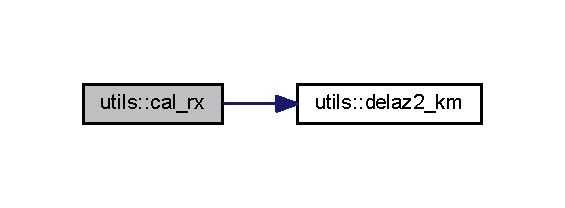
\includegraphics[width=271pt]{namespaceutils_aa1727e2ba89368130186d248fd7b71b4_cgraph}
\end{center}
\end{figure}


\hypertarget{namespaceutils_aa0f32919ddbbde1b5238425529660459}{}\index{utils@{utils}!deg2km\+\_\+simple@{deg2km\+\_\+simple}}
\index{deg2km\+\_\+simple@{deg2km\+\_\+simple}!utils@{utils}}
\subsubsection[{deg2km\+\_\+simple(vn, ve, alat\+\_\+sta, alon\+\_\+sta,                                           alat\+\_\+ref, alon\+\_\+ref)}]{\setlength{\rightskip}{0pt plus 5cm}subroutine utils\+::deg2km\+\_\+simple (
\begin{DoxyParamCaption}
\item[{real(8)}]{vn, }
\item[{real(8)}]{ve, }
\item[{real(8)}]{alat\+\_\+sta, }
\item[{real(8)}]{alon\+\_\+sta, }
\item[{real(8)}]{alat\+\_\+ref, }
\item[{real(8)}]{alon\+\_\+ref}
\end{DoxyParamCaption}
)}\label{namespaceutils_aa0f32919ddbbde1b5238425529660459}
\hypertarget{namespaceutils_aa1dce66e1b3b67f4ff37fa7a949cb7b4}{}\index{utils@{utils}!delaz2\+\_\+km@{delaz2\+\_\+km}}
\index{delaz2\+\_\+km@{delaz2\+\_\+km}!utils@{utils}}
\subsubsection[{delaz2\+\_\+km(y1, x1, y2, x2, delta, az)}]{\setlength{\rightskip}{0pt plus 5cm}subroutine utils\+::delaz2\+\_\+km (
\begin{DoxyParamCaption}
\item[{real(8), intent(in)}]{y1, }
\item[{real(8), intent(in)}]{x1, }
\item[{real(8), intent(in)}]{y2, }
\item[{real(8), intent(in)}]{x2, }
\item[{real(8), intent(out)}]{delta, }
\item[{real(8), intent(out)}]{az}
\end{DoxyParamCaption}
)}\label{namespaceutils_aa1dce66e1b3b67f4ff37fa7a949cb7b4}
\hypertarget{namespaceutils_a568d3767bca697c86b861637a25888f8}{}\index{utils@{utils}!deltacdf@{deltacdf}}
\index{deltacdf@{deltacdf}!utils@{utils}}
\subsubsection[{deltacdf(x)}]{\setlength{\rightskip}{0pt plus 5cm}elemental real(8) function utils\+::deltacdf (
\begin{DoxyParamCaption}
\item[{real(8), intent(in)}]{x}
\end{DoxyParamCaption}
)}\label{namespaceutils_a568d3767bca697c86b861637a25888f8}
\hypertarget{namespaceutils_af6906785e7d185fbdf7034969aababc4}{}\index{utils@{utils}!dist\+\_\+rup\+\_\+seg@{dist\+\_\+rup\+\_\+seg}}
\index{dist\+\_\+rup\+\_\+seg@{dist\+\_\+rup\+\_\+seg}!utils@{utils}}
\subsubsection[{dist\+\_\+rup\+\_\+seg(\+Rrup, Rjb, Rx, coor, Ztor, strike, dip, rup\+\_\+wid)}]{\setlength{\rightskip}{0pt plus 5cm}subroutine utils\+::dist\+\_\+rup\+\_\+seg (
\begin{DoxyParamCaption}
\item[{real(8)}]{Rrup, }
\item[{real(8)}]{Rjb, }
\item[{real(8)}]{Rx, }
\item[{real(8), dimension(2,2)}]{coor, }
\item[{real(8)}]{Ztor, }
\item[{real(8)}]{strike, }
\item[{real(8)}]{dip, }
\item[{real(8)}]{rup\+\_\+wid}
\end{DoxyParamCaption}
)}\label{namespaceutils_af6906785e7d185fbdf7034969aababc4}


Here is the call graph for this function\+:
\nopagebreak
\begin{figure}[H]
\begin{center}
\leavevmode
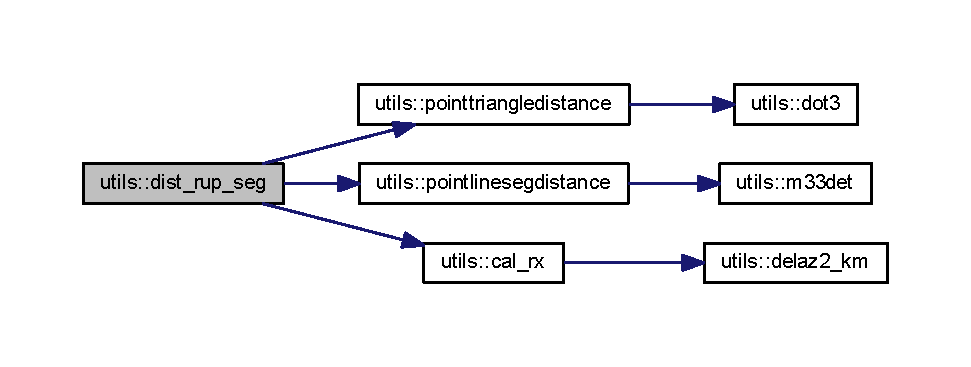
\includegraphics[width=350pt]{namespaceutils_af6906785e7d185fbdf7034969aababc4_cgraph}
\end{center}
\end{figure}


\hypertarget{namespaceutils_a3dfc1e25be8aa02534fda1a437ec9855}{}\index{utils@{utils}!dist\+\_\+rup\+\_\+set@{dist\+\_\+rup\+\_\+set}}
\index{dist\+\_\+rup\+\_\+set@{dist\+\_\+rup\+\_\+set}!utils@{utils}}
\subsubsection[{dist\+\_\+rup\+\_\+set(\+Rrup, Rjb, Rx, coor, Ztor, strike, dip, rup\+\_\+wid)}]{\setlength{\rightskip}{0pt plus 5cm}subroutine utils\+::dist\+\_\+rup\+\_\+set (
\begin{DoxyParamCaption}
\item[{real(8)}]{Rrup, }
\item[{real(8)}]{Rjb, }
\item[{real(8)}]{Rx, }
\item[{real(8), dimension(\+:,\+:), allocatable}]{coor, }
\item[{real(8)}]{Ztor, }
\item[{real(8)}]{strike, }
\item[{real(8)}]{dip, }
\item[{real(8)}]{rup\+\_\+wid}
\end{DoxyParamCaption}
)}\label{namespaceutils_a3dfc1e25be8aa02534fda1a437ec9855}


Here is the call graph for this function\+:
\nopagebreak
\begin{figure}[H]
\begin{center}
\leavevmode
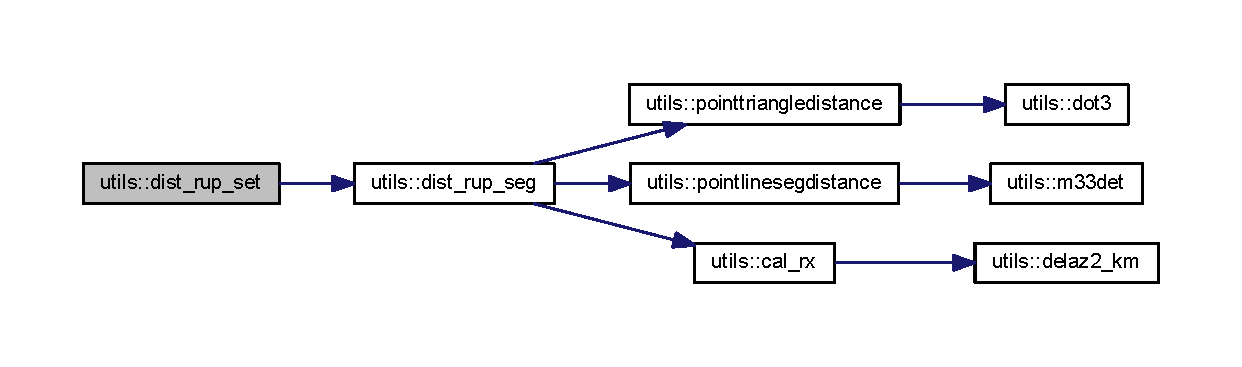
\includegraphics[width=350pt]{namespaceutils_a3dfc1e25be8aa02534fda1a437ec9855_cgraph}
\end{center}
\end{figure}


\hypertarget{namespaceutils_ab5a1a9ca34591c37c7fb606189317e16}{}\index{utils@{utils}!dot3@{dot3}}
\index{dot3@{dot3}!utils@{utils}}
\subsubsection[{dot3(x, y)}]{\setlength{\rightskip}{0pt plus 5cm}real(8) function utils\+::dot3 (
\begin{DoxyParamCaption}
\item[{real(8), dimension(3)}]{x, }
\item[{real(8), dimension(3)}]{y}
\end{DoxyParamCaption}
)}\label{namespaceutils_ab5a1a9ca34591c37c7fb606189317e16}
\hypertarget{namespaceutils_ae3d121578601cfdb0b2687656ea19761}{}\index{utils@{utils}!interp\+\_\+coeff@{interp\+\_\+coeff}}
\index{interp\+\_\+coeff@{interp\+\_\+coeff}!utils@{utils}}
\subsubsection[{interp\+\_\+coeff(x1, x2, y1, y2, x, y, iflag)}]{\setlength{\rightskip}{0pt plus 5cm}subroutine utils\+::interp\+\_\+coeff (
\begin{DoxyParamCaption}
\item[{real(8)}]{x1, }
\item[{real(8)}]{x2, }
\item[{real(8)}]{y1, }
\item[{real(8)}]{y2, }
\item[{real(8)}]{x, }
\item[{real(8)}]{y, }
\item[{integer}]{iflag}
\end{DoxyParamCaption}
)}\label{namespaceutils_ae3d121578601cfdb0b2687656ea19761}
\hypertarget{namespaceutils_a6c61290deedf912e6810628145911f85}{}\index{utils@{utils}!locate@{locate}}
\index{locate@{locate}!utils@{utils}}
\subsubsection[{locate(ibin, edge, x)}]{\setlength{\rightskip}{0pt plus 5cm}subroutine utils\+::locate (
\begin{DoxyParamCaption}
\item[{integer}]{ibin, }
\item[{real(8), dimension(\+:), allocatable}]{edge, }
\item[{real(8)}]{x}
\end{DoxyParamCaption}
)}\label{namespaceutils_a6c61290deedf912e6810628145911f85}
\hypertarget{namespaceutils_a64e66c94f05898717cbc1863f70c9be1}{}\index{utils@{utils}!m22det@{m22det}}
\index{m22det@{m22det}!utils@{utils}}
\subsubsection[{m22det(\+A)}]{\setlength{\rightskip}{0pt plus 5cm}double precision function utils\+::m22det (
\begin{DoxyParamCaption}
\item[{double precision, dimension(2,2), intent(in)}]{A}
\end{DoxyParamCaption}
)}\label{namespaceutils_a64e66c94f05898717cbc1863f70c9be1}
\hypertarget{namespaceutils_a9bad87c0b79a45b5c6e6bbfcb2c6a126}{}\index{utils@{utils}!m33det@{m33det}}
\index{m33det@{m33det}!utils@{utils}}
\subsubsection[{m33det(\+A)}]{\setlength{\rightskip}{0pt plus 5cm}double precision function utils\+::m33det (
\begin{DoxyParamCaption}
\item[{double precision, dimension(3,3), intent(in)}]{A}
\end{DoxyParamCaption}
)}\label{namespaceutils_a9bad87c0b79a45b5c6e6bbfcb2c6a126}
\hypertarget{namespaceutils_aa41cc7594a2b7ecd3f3931859172f175}{}\index{utils@{utils}!normcdf@{normcdf}}
\index{normcdf@{normcdf}!utils@{utils}}
\subsubsection[{normcdf(x)}]{\setlength{\rightskip}{0pt plus 5cm}elemental real(8) function utils\+::normcdf (
\begin{DoxyParamCaption}
\item[{real(8), intent(in)}]{x}
\end{DoxyParamCaption}
)}\label{namespaceutils_aa41cc7594a2b7ecd3f3931859172f175}
\hypertarget{namespaceutils_aa037ebfaff3336105e73f563fdab02a8}{}\index{utils@{utils}!pointlinesegdistance@{pointlinesegdistance}}
\index{pointlinesegdistance@{pointlinesegdistance}!utils@{utils}}
\subsubsection[{pointlinesegdistance(a, b, x, dist)}]{\setlength{\rightskip}{0pt plus 5cm}subroutine utils\+::pointlinesegdistance (
\begin{DoxyParamCaption}
\item[{real(8), dimension(2)}]{a, }
\item[{real(8), dimension(2)}]{b, }
\item[{real(8), dimension(2), intent(in)}]{x, }
\item[{real(8), intent(out)}]{dist}
\end{DoxyParamCaption}
)}\label{namespaceutils_aa037ebfaff3336105e73f563fdab02a8}


Here is the call graph for this function\+:
\nopagebreak
\begin{figure}[H]
\begin{center}
\leavevmode
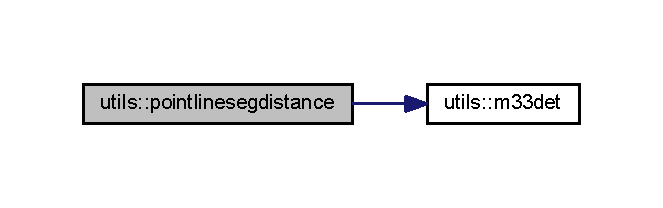
\includegraphics[width=318pt]{namespaceutils_aa037ebfaff3336105e73f563fdab02a8_cgraph}
\end{center}
\end{figure}


\hypertarget{namespaceutils_aebfee5643eb6828d1b6fd64229189af0}{}\index{utils@{utils}!pointtriangledistance@{pointtriangledistance}}
\index{pointtriangledistance@{pointtriangledistance}!utils@{utils}}
\subsubsection[{pointtriangledistance(\+T\+R\+I1, T\+R\+I2, T\+R\+I3, P, dist)}]{\setlength{\rightskip}{0pt plus 5cm}subroutine utils\+::pointtriangledistance (
\begin{DoxyParamCaption}
\item[{real(8), dimension(3), intent(in)}]{T\+R\+I1, }
\item[{real(8), dimension(3), intent(in)}]{T\+R\+I2, }
\item[{real(8), dimension(3), intent(in)}]{T\+R\+I3, }
\item[{real(8), dimension(3), intent(in)}]{P, }
\item[{real(8), intent(out)}]{dist}
\end{DoxyParamCaption}
)}\label{namespaceutils_aebfee5643eb6828d1b6fd64229189af0}


Here is the call graph for this function\+:
\nopagebreak
\begin{figure}[H]
\begin{center}
\leavevmode
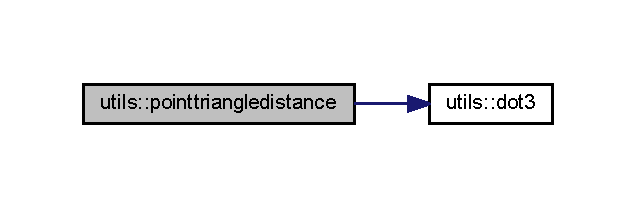
\includegraphics[width=305pt]{namespaceutils_aebfee5643eb6828d1b6fd64229189af0_cgraph}
\end{center}
\end{figure}


\hypertarget{namespaceutils_a47c34e02c3a6ca718ff160f085117f47}{}\index{utils@{utils}!prob\+\_\+exceed@{prob\+\_\+exceed}}
\index{prob\+\_\+exceed@{prob\+\_\+exceed}!utils@{utils}}
\subsubsection[{prob\+\_\+exceed(p\+\_\+exceed, m\+\_\+eps, m\+\_\+aleatory\+\_\+distribution, trunclevel)}]{\setlength{\rightskip}{0pt plus 5cm}subroutine utils\+::prob\+\_\+exceed (
\begin{DoxyParamCaption}
\item[{real(8)}]{p\+\_\+exceed, }
\item[{real(8)}]{m\+\_\+eps, }
\item[{integer}]{m\+\_\+aleatory\+\_\+distribution, }
\item[{real(8)}]{trunclevel}
\end{DoxyParamCaption}
)}\label{namespaceutils_a47c34e02c3a6ca718ff160f085117f47}


Here is the call graph for this function\+:
\nopagebreak
\begin{figure}[H]
\begin{center}
\leavevmode
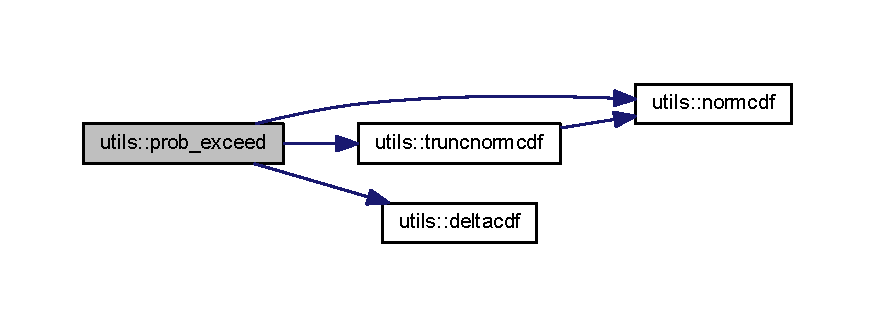
\includegraphics[width=350pt]{namespaceutils_a47c34e02c3a6ca718ff160f085117f47_cgraph}
\end{center}
\end{figure}


\hypertarget{namespaceutils_ac313e8810c0e461aa91b7299c8fba4be}{}\index{utils@{utils}!truncnormcdf@{truncnormcdf}}
\index{truncnormcdf@{truncnormcdf}!utils@{utils}}
\subsubsection[{truncnormcdf(x, a, b, z)}]{\setlength{\rightskip}{0pt plus 5cm}subroutine utils\+::truncnormcdf (
\begin{DoxyParamCaption}
\item[{real(8), intent(in)}]{x, }
\item[{real(8), intent(in)}]{a, }
\item[{real(8), intent(in)}]{b, }
\item[{real(8), intent(out)}]{z}
\end{DoxyParamCaption}
)}\label{namespaceutils_ac313e8810c0e461aa91b7299c8fba4be}


Here is the call graph for this function\+:
\nopagebreak
\begin{figure}[H]
\begin{center}
\leavevmode
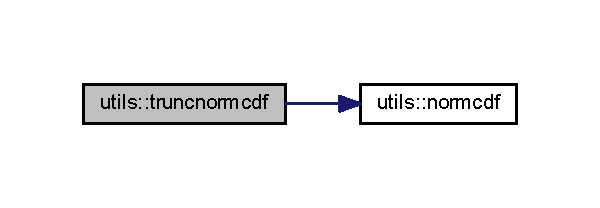
\includegraphics[width=288pt]{namespaceutils_ac313e8810c0e461aa91b7299c8fba4be_cgraph}
\end{center}
\end{figure}



\chapter{File Documentation}
\hypertarget{const__module_8f90}{}\section{const\+\_\+module.\+f90 File Reference}
\label{const__module_8f90}\index{const\+\_\+module.\+f90@{const\+\_\+module.\+f90}}
\subsection*{Modules}
\begin{DoxyCompactItemize}
\item 
module \hyperlink{namespaceconst__module}{const\+\_\+module}
\end{DoxyCompactItemize}
\subsection*{Variables}
\begin{DoxyCompactItemize}
\item 
real(8), parameter \hyperlink{namespaceconst__module_a6e2d7a0e80dfe577ca95736d3e143899}{const\+\_\+module\+::pi} = 3.\+14159265358979
\item 
real(8), parameter \hyperlink{namespaceconst__module_a87cf12ab3afb0ddc5f58492d1fb1d828}{const\+\_\+module\+::deg2rad} = 0.\+0174532925199433
\item 
real(8), parameter \hyperlink{namespaceconst__module_a61843a48c8dec76293f423c682c8d772}{const\+\_\+module\+::rad2deg} = 57.\+2957795130823
\item 
real(8), parameter \hyperlink{namespaceconst__module_aa70be203aa6a91ce3961b81a6eae1e60}{const\+\_\+module\+::sqrt2\+\_\+inv} = 0.\+707106781186547
\item 
real(8), parameter \hyperlink{namespaceconst__module_ab766035166a55b031df25669f66e7b06}{const\+\_\+module\+::earth\+\_\+r} = 6371.\+0
\item 
integer, parameter \hyperlink{namespaceconst__module_afdf6c6b7ffea232bbc86b7ffef8298dc}{const\+\_\+module\+::ss} = 1
\item 
integer, parameter \hyperlink{namespaceconst__module_a2fac1c74f2a81234dec392f6ad1c73ea}{const\+\_\+module\+::rv} = 2
\item 
integer, parameter \hyperlink{namespaceconst__module_a45c7ab4515e2c0068ca69e5f4fed8a51}{const\+\_\+module\+::nm} = 3
\item 
integer, parameter \hyperlink{namespaceconst__module_a437f551584bfdf420d4b28c829759eb5}{const\+\_\+module\+::na} = 4
\item 
integer, parameter \hyperlink{namespaceconst__module_a760935a100ba2e8695aa777f582d5a61}{const\+\_\+module\+::wc94} = 1
\item 
integer, parameter \hyperlink{namespaceconst__module_a28954bb32bf9368bbb5569a257603c57}{const\+\_\+module\+::peer} = 2
\item 
integer, parameter \hyperlink{namespaceconst__module_a6d9b6ff754fe58527edcaea132c3d736}{const\+\_\+module\+::ceus} = 3
\item 
integer, parameter \hyperlink{namespaceconst__module_aac415d96f710c33f0228284d6f5504c9}{const\+\_\+module\+::point} = 4
\item 
integer, parameter \hyperlink{namespaceconst__module_a7b2347a542b2eda2b6841e1d9fdf19f4}{const\+\_\+module\+::exponential} = 1
\item 
integer, parameter \hyperlink{namespaceconst__module_ab9dc6742ce1e2309dd194ecdd254779d}{const\+\_\+module\+::characteristic} = 2
\item 
integer, parameter \hyperlink{namespaceconst__module_a6bed9e9fc42a9b205a9214865ad145f5}{const\+\_\+module\+::delta} = 3
\item 
integer, parameter \hyperlink{namespaceconst__module_ad7dece49d5a2db833c491ea2eed54f52}{const\+\_\+module\+::deg} = 1
\item 
integer, parameter \hyperlink{namespaceconst__module_a4e8504d7945ca96447c578c95644bd5a}{const\+\_\+module\+::km} = 2
\item 
integer, parameter \hyperlink{namespaceconst__module_a83696a36c5a2e83e44cbfbbc479717a9}{const\+\_\+module\+::sadigh97} = 1
\item 
integer, parameter \hyperlink{namespaceconst__module_ac32c40069d129a7d06c22292afaae3ba}{const\+\_\+module\+::cy14} = 2
\item 
integer, parameter \hyperlink{namespaceconst__module_a91a738fc17a72ffc4e34e5141cccc469}{const\+\_\+module\+::uniform} = 1
\item 
integer, parameter \hyperlink{namespaceconst__module_a7e2946932c4a8471477923bc49aeafe4}{const\+\_\+module\+::triangular} = 2
\item 
integer, parameter \hyperlink{namespaceconst__module_a8010dcce5207fede7f1da8dbde0b5be8}{const\+\_\+module\+::normal} = 1
\item 
integer, parameter \hyperlink{namespaceconst__module_a3895bfacad51cb8237e9cae087b1663a}{const\+\_\+module\+::trunc\+\_\+normal} = 2
\item 
integer, parameter \hyperlink{namespaceconst__module_a0a0ee9e64316ae52e9c539987c5d18d5}{const\+\_\+module\+::heaviside} = 3
\end{DoxyCompactItemize}

\hypertarget{flt__module_8f90}{}\section{flt\+\_\+module.\+f90 File Reference}
\label{flt__module_8f90}\index{flt\+\_\+module.\+f90@{flt\+\_\+module.\+f90}}
\subsection*{Modules}
\begin{DoxyCompactItemize}
\item 
module \hyperlink{namespaceflt__module}{flt\+\_\+module}
\end{DoxyCompactItemize}
\subsection*{Functions/\+Subroutines}
\begin{DoxyCompactItemize}
\item 
subroutine \hyperlink{namespaceflt__module_a36fbe983f26cb385897a0f3b3a69b374}{flt\+\_\+module\+::mag\+\_\+freq\+\_\+distribution} ()
\item 
subroutine \hyperlink{flt__module_8f90_a97aa7eb6fea0093dd73109fe014535b4}{mfd\+\_\+delta} ()
\item 
subroutine \hyperlink{flt__module_8f90_a57006c14043e293ddc4506dfe0291848}{mfd\+\_\+exp} ()
\item 
subroutine \hyperlink{flt__module_8f90_abcae43af287f888ab306c973bdfa32e1}{mfd\+\_\+char} ()
\item 
subroutine \hyperlink{namespaceflt__module_adf3a48955b957b3900c168b85a7e3a7f}{flt\+\_\+module\+::unit\+\_\+conversion} ()
\item 
subroutine \hyperlink{namespaceflt__module_abdb1848f76f2f97490cbb813742463bb}{flt\+\_\+module\+::caldepthprob} ()
\item 
subroutine \hyperlink{namespaceflt__module_a7c28beda425cae19654ab1d770575fa9}{flt\+\_\+module\+::deg2km\+\_\+model} ()
\item 
subroutine \hyperlink{namespaceflt__module_a5fa0cac3fd11ee99069c21930a0e2fa4}{flt\+\_\+module\+::align\+\_\+model} ()
\item 
subroutine \hyperlink{namespaceflt__module_a70e82d6c4a8cbb15e934c5b846b3f2fd}{flt\+\_\+module\+::flt\+\_\+ini} ()
\item 
subroutine \hyperlink{namespaceflt__module_aea512cba753c29d842ade7e80af288dc}{flt\+\_\+module\+::cal\+\_\+p\+\_\+locd\+\_\+arr} ()
\item 
subroutine \hyperlink{namespaceflt__module_ae0fae05513f5a50898cdd23f18cee48e}{flt\+\_\+module\+::cal\+\_\+coor\+\_\+d} ()
\item 
subroutine \hyperlink{namespaceflt__module_a5e554053b0a794d5027652daae033cbb}{flt\+\_\+module\+::rupture\+\_\+location} ()
\item 
subroutine \hyperlink{namespaceflt__module_a4df7cbbee97b24416c4834d0da1d86f5}{flt\+\_\+module\+::locate\+\_\+rupture} (S1\+\_\+local, S2\+\_\+local, rup\+\_\+coor)
\item 
subroutine \hyperlink{namespaceflt__module_a03121e683f2ec0d996e20de582b4a47c}{flt\+\_\+module\+::mw2arup} ()
\end{DoxyCompactItemize}
\subsection*{Variables}
\begin{DoxyCompactItemize}
\item 
real(8), dimension(\+:), allocatable \hyperlink{namespaceflt__module_aca5726712ea516198b181e7cb2f58a79}{flt\+\_\+module\+::flt\+\_\+len\+\_\+seg}
\item 
real(8), dimension(\+:), allocatable \hyperlink{namespaceflt__module_afe7ee1528f7162ad84a3517be2962885}{flt\+\_\+module\+::flt\+\_\+az\+\_\+seg}
\item 
real(8), dimension(\+:,\+:), allocatable \hyperlink{namespaceflt__module_a5f040c388185e1ef250084d5c59d41e9}{flt\+\_\+module\+::flt\+\_\+coor}
\item 
real(8), dimension(\+:), allocatable \hyperlink{namespaceflt__module_ade0f97d7261ffc38567aa16de68c1583}{flt\+\_\+module\+::flt\+\_\+s\+\_\+corner}
\item 
real(8), dimension(2) \hyperlink{namespaceflt__module_a2aeddbabcca2c320d94712a5ef502b79}{flt\+\_\+module\+::site\+\_\+coor}
\item 
real(8), dimension(\+:), allocatable \hyperlink{namespaceflt__module_ab5c2fb389cfd0080d938d50ef55e28ef}{flt\+\_\+module\+::rup\+\_\+top}
\item 
real(8), dimension(\+:,\+:), allocatable \hyperlink{namespaceflt__module_afbf76baeddad45d761cc805c838b369a}{flt\+\_\+module\+::rup\+\_\+coor}
\item 
real(8), dimension(\+:,\+:), allocatable \hyperlink{namespaceflt__module_a46387202eab4affb664fabc1dfbc3523}{flt\+\_\+module\+::coor\+\_\+d}
\item 
real(8), dimension(\+:), allocatable \hyperlink{namespaceflt__module_a388db17b48dfcaeb0b4c53d1a23f83b6}{flt\+\_\+module\+::s1}
\item 
real(8), dimension(\+:), allocatable \hyperlink{namespaceflt__module_a774958e9c5ad266c9faed76a724e27ac}{flt\+\_\+module\+::s2}
\item 
real(8), dimension(\+:), allocatable \hyperlink{namespaceflt__module_a3ae9412ace7bafcdc16443a1de523c08}{flt\+\_\+module\+::p\+\_\+locd\+\_\+arr}
\item 
real(8), dimension(\+:), allocatable \hyperlink{namespaceflt__module_a758f2d6ebaadfe7af02eddd7ab5e4bdd}{flt\+\_\+module\+::mag\+\_\+inc\+\_\+0}
\item 
real(8), dimension(\+:), allocatable \hyperlink{namespaceflt__module_a3aa16b477093fff931adc3d47efb4391}{flt\+\_\+module\+::rate\+\_\+inc\+\_\+0}
\item 
real(8), dimension(\+:), allocatable \hyperlink{namespaceflt__module_af9892b4dca9fdd6644278654eb95f0d2}{flt\+\_\+module\+::mag\+\_\+inc}
\item 
real(8), dimension(\+:), allocatable \hyperlink{namespaceflt__module_af4abd22305b27392695e298e409485eb}{flt\+\_\+module\+::rate\+\_\+inc}
\item 
real(8) \hyperlink{namespaceflt__module_a5afcf609fce08da82c3c6f3c6ae623d1}{flt\+\_\+module\+::flt\+\_\+area}
\item 
real(8) \hyperlink{namespaceflt__module_a4bc1d05951c8d1ad1263099b2168fc52}{flt\+\_\+module\+::flt\+\_\+len}
\item 
real(8) \hyperlink{namespaceflt__module_a0a0ca2180f3d4b230a85f4e74898c1ab}{flt\+\_\+module\+::flt\+\_\+wid}
\item 
real(8) \hyperlink{namespaceflt__module_a5f628ae600d8550ab693d874d7a26bb0}{flt\+\_\+module\+::flt\+\_\+strike\+\_\+deg}
\item 
real(8) \hyperlink{namespaceflt__module_a618a9014909e559bdbedf80be8a159a3}{flt\+\_\+module\+::flt\+\_\+strike\+\_\+rad}
\item 
real(8) \hyperlink{namespaceflt__module_ad4dbd8fe640ed7c127b993e51b31c2cb}{flt\+\_\+module\+::step\+\_\+d}
\item 
real(8) \hyperlink{namespaceflt__module_aac3ac3d5dda31c71db0f70b6c04bde99}{flt\+\_\+module\+::step\+\_\+s}
\item 
real(8) \hyperlink{namespaceflt__module_a5a750dfe01760a5134b5cd98aa924b01}{flt\+\_\+module\+::step\+\_\+d\+\_\+trial}
\item 
real(8) \hyperlink{namespaceflt__module_abbc6ad6d8104d02669bab58b22654f6b}{flt\+\_\+module\+::step\+\_\+s\+\_\+trial}
\item 
real(8) \hyperlink{namespaceflt__module_aa83583fdd38e91b447b8fbf1ae9f833c}{flt\+\_\+module\+::rup\+\_\+len}
\item 
real(8) \hyperlink{namespaceflt__module_a5cbe7cb918ea3ecbe35270bdcc9ab63d}{flt\+\_\+module\+::rup\+\_\+wid}
\item 
real(8) \hyperlink{namespaceflt__module_aec90f89a37148a6fe2fa52df737b51ef}{flt\+\_\+module\+::rup\+\_\+area}
\item 
real(8) \hyperlink{namespaceflt__module_acb649d537953bd575e6bbded75b6c99b}{flt\+\_\+module\+::rup\+\_\+len\+\_\+trial}
\item 
real(8) \hyperlink{namespaceflt__module_a6cefaab59a5e1f02e62505b132fe9384}{flt\+\_\+module\+::rup\+\_\+wid\+\_\+trial}
\item 
real(8) \hyperlink{namespaceflt__module_af824d404f5d8ef8f21222c648b493389}{flt\+\_\+module\+::rup\+\_\+area\+\_\+trial}
\item 
integer \hyperlink{namespaceflt__module_a82fbb8ec3230fb344b2e8970e95398e3}{flt\+\_\+module\+::n\+\_\+locd}
\item 
integer \hyperlink{namespaceflt__module_ab114b19843b4c7f6c795898a67157717}{flt\+\_\+module\+::i\+\_\+locd}
\item 
integer \hyperlink{namespaceflt__module_a544a94f997804736b60b9989c7489732}{flt\+\_\+module\+::n\+\_\+locs}
\item 
integer \hyperlink{namespaceflt__module_ab04ec1f028778d49315cb1d0f6e80941}{flt\+\_\+module\+::i\+\_\+locs}
\item 
integer \hyperlink{namespaceflt__module_ab23ea8eb58ad8e18929cf668eb01f663}{flt\+\_\+module\+::n\+\_\+cor}
\item 
integer \hyperlink{namespaceflt__module_a74639d2c8f137bceff8db7f162301d8c}{flt\+\_\+module\+::i\+\_\+seg}
\item 
real(8) \hyperlink{namespaceflt__module_a3a9896b28d0823ab1f9c8bda7380c0d9}{flt\+\_\+module\+::step\+\_\+d\+\_\+v}
\item 
real(8) \hyperlink{namespaceflt__module_a2bbb6ee47643b88f63a980bf4f075ad5}{flt\+\_\+module\+::step\+\_\+d\+\_\+h}
\item 
real(8) \hyperlink{namespaceflt__module_afaa001d959f566926be3b2e7383fa244}{flt\+\_\+module\+::step\+\_\+d\+\_\+hc}
\item 
real(8) \hyperlink{namespaceflt__module_a5e5aaec050d5c1fa09b359dc2b162532}{flt\+\_\+module\+::step\+\_\+d\+\_\+hs}
\item 
real(8) \hyperlink{namespaceflt__module_ac1c817f0b45b42ee735df0300075b47e}{flt\+\_\+module\+::p\+\_\+locs}
\item 
real(8) \hyperlink{namespaceflt__module_a9a55926b369374d66caf682a539d8acf}{flt\+\_\+module\+::p\+\_\+locd}
\item 
real(8) \hyperlink{namespaceflt__module_a9e6d611f8124986d8547149562e07e40}{flt\+\_\+module\+::ftop}
\item 
real(8) \hyperlink{namespaceflt__module_aa0b3754bd3b678669c3b99f861359208}{flt\+\_\+module\+::mw}
\item 
real(8) \hyperlink{namespaceflt__module_ac0a06739ec2f31f13ad0b2213797e9c7}{flt\+\_\+module\+::rate}
\item 
real(8) \hyperlink{namespaceflt__module_aacc666d4125c94c8ff0b54e1a6fac18b}{flt\+\_\+module\+::rrup}
\item 
real(8) \hyperlink{namespaceflt__module_a61bb108f64be27cd6e6b621bd0d2be66}{flt\+\_\+module\+::rjb}
\item 
real(8) \hyperlink{namespaceflt__module_a8fa2cff4d9d0c963d1d2e99f399211c5}{flt\+\_\+module\+::rx}
\item 
integer \hyperlink{namespaceflt__module_a5e6a726815330fe30804c2cfb77e2651}{flt\+\_\+module\+::i\+\_\+mag}
\item 
integer \hyperlink{namespaceflt__module_ac480b7d0327ba835996ed5a35a3c6ec4}{flt\+\_\+module\+::n\+\_\+mag}
\item 
integer \hyperlink{namespaceflt__module_a922b2ed6f3dff53fad4a824cde4270fd}{flt\+\_\+module\+::i\+\_\+mag\+\_\+bin}
\item 
integer \hyperlink{namespaceflt__module_a9480fc2f60b62f2eb903d45f90e0dc73}{flt\+\_\+module\+::i\+\_\+dist\+\_\+bin}
\item 
integer \hyperlink{namespaceflt__module_a4bb764374a373b9dea720cedee5f208a}{flt\+\_\+module\+::i\+\_\+eps\+\_\+bin}
\item 
integer \hyperlink{namespaceflt__module_aa1dd9d9c50f40c03cb2d3e6772366e77}{flt\+\_\+module\+::i\+\_\+freq}
\item 
integer \hyperlink{namespaceflt__module_ae179cb5e3d011707ce0742d9c49df852}{flt\+\_\+module\+::i\+\_\+inten}
\item 
real(8) \hyperlink{namespaceflt__module_ab88c9c308585340c18213d3778e152a9}{flt\+\_\+module\+::tin}
\end{DoxyCompactItemize}


\subsection{Function/\+Subroutine Documentation}
\hypertarget{flt__module_8f90_abcae43af287f888ab306c973bdfa32e1}{}\index{flt\+\_\+module.\+f90@{flt\+\_\+module.\+f90}!mfd\+\_\+char@{mfd\+\_\+char}}
\index{mfd\+\_\+char@{mfd\+\_\+char}!flt\+\_\+module.\+f90@{flt\+\_\+module.\+f90}}
\subsubsection[{mfd\+\_\+char()}]{\setlength{\rightskip}{0pt plus 5cm}subroutine mag\+\_\+freq\+\_\+distribution\+::mfd\+\_\+char (
\begin{DoxyParamCaption}
{}
\end{DoxyParamCaption}
)}\label{flt__module_8f90_abcae43af287f888ab306c973bdfa32e1}
\hypertarget{flt__module_8f90_a97aa7eb6fea0093dd73109fe014535b4}{}\index{flt\+\_\+module.\+f90@{flt\+\_\+module.\+f90}!mfd\+\_\+delta@{mfd\+\_\+delta}}
\index{mfd\+\_\+delta@{mfd\+\_\+delta}!flt\+\_\+module.\+f90@{flt\+\_\+module.\+f90}}
\subsubsection[{mfd\+\_\+delta()}]{\setlength{\rightskip}{0pt plus 5cm}subroutine mag\+\_\+freq\+\_\+distribution\+::mfd\+\_\+delta (
\begin{DoxyParamCaption}
{}
\end{DoxyParamCaption}
)}\label{flt__module_8f90_a97aa7eb6fea0093dd73109fe014535b4}
\hypertarget{flt__module_8f90_a57006c14043e293ddc4506dfe0291848}{}\index{flt\+\_\+module.\+f90@{flt\+\_\+module.\+f90}!mfd\+\_\+exp@{mfd\+\_\+exp}}
\index{mfd\+\_\+exp@{mfd\+\_\+exp}!flt\+\_\+module.\+f90@{flt\+\_\+module.\+f90}}
\subsubsection[{mfd\+\_\+exp()}]{\setlength{\rightskip}{0pt plus 5cm}subroutine mag\+\_\+freq\+\_\+distribution\+::mfd\+\_\+exp (
\begin{DoxyParamCaption}
{}
\end{DoxyParamCaption}
)}\label{flt__module_8f90_a57006c14043e293ddc4506dfe0291848}

\hypertarget{_g_m_p_e__module_8f90}{}\section{G\+M\+P\+E\+\_\+module.\+f90 File Reference}
\label{_g_m_p_e__module_8f90}\index{G\+M\+P\+E\+\_\+module.\+f90@{G\+M\+P\+E\+\_\+module.\+f90}}
\subsection*{Modules}
\begin{DoxyCompactItemize}
\item 
module \hyperlink{namespacegmpe__module}{gmpe\+\_\+module}
\end{DoxyCompactItemize}
\subsection*{Functions/\+Subroutines}
\begin{DoxyCompactItemize}
\item 
subroutine \hyperlink{namespacegmpe__module_a5f684874da41cb0160ab7c0473b1adf5}{gmpe\+\_\+module\+::gmpe\+\_\+interface} (m\+\_\+gmpe\+\_\+name, Tin, Mw, m\+\_\+sof, Rrup, Rjb, Rx, Ztor, dip,                                           Vs30, Z10, gmpe\+\_\+params, gmpe\+\_\+opts,                                           ln\+Sa, Sigma)
\item 
subroutine \hyperlink{namespacegmpe__module_a3a1c1fc463d12762d4dcc724f90f876d}{gmpe\+\_\+module\+::gmpe\+\_\+sadigh97} (ln\+Sa, Sigma, M, Rrup, Tin, m\+\_\+\+S\+O\+F)
\item 
subroutine \hyperlink{namespacegmpe__module_a908fe9e90b79ba090e108746e35b4b02}{gmpe\+\_\+module\+::gmpe\+\_\+cy14} (M, T, Rrup, Rjb, Rx, Ztor, dip, m\+\_\+\+S\+O\+F, Z10, Vs30, gmpe\+\_\+params, gmpe\+\_\+opts, ln\+Sa, sigma)
\item 
subroutine \hyperlink{namespacegmpe__module_a2b7ab2b80fab7e94cfd35a2e5652bc5a}{gmpe\+\_\+module\+::cy\+\_\+2014\+\_\+sub} (M, ip, R\+\_\+\+R\+U\+P, R\+\_\+\+J\+B, Rx, Ztor, delta, F\+\_\+\+R\+V, F\+\_\+\+N\+M, H\+W, Z10, Vs30, F\+V\+S30, region, d\+\_\+\+D\+P\+P, ln\+Sa, sigma)
\item 
subroutine \hyperlink{namespacegmpe__module_aaef04e7344731f519aba25dbde1bfbc8}{gmpe\+\_\+module\+::per\+\_\+indx\+\_\+cy14} (per, per\+\_\+indx)
\end{DoxyCompactItemize}

\hypertarget{input__module_8f90}{}\section{input\+\_\+module.\+f90 File Reference}
\label{input__module_8f90}\index{input\+\_\+module.\+f90@{input\+\_\+module.\+f90}}
\subsection*{Modules}
\begin{DoxyCompactItemize}
\item 
module \hyperlink{namespaceinput__module}{input\+\_\+module}
\end{DoxyCompactItemize}
\subsection*{Functions/\+Subroutines}
\begin{DoxyCompactItemize}
\item 
subroutine \hyperlink{namespaceinput__module_a00c4a5d066f42d27b85b05a38bed5160}{input\+\_\+module\+::read\+\_\+input} ()
\item 
subroutine \hyperlink{namespaceinput__module_a07cd15a61e7f02633605f2f442ceb937}{input\+\_\+module\+::read\+\_\+site} ()
\item 
subroutine \hyperlink{namespaceinput__module_afa2966a0e5fac1ac508ed7aed4f0a3d8}{input\+\_\+module\+::read\+\_\+frequency} ()
\item 
subroutine \hyperlink{namespaceinput__module_a0d373b7166a3c84647da12172e1ea635}{input\+\_\+module\+::read\+\_\+fault\+\_\+trace} ()
\item 
subroutine \hyperlink{namespaceinput__module_a1e706b509f806cf51ec52d88f6be16f5}{input\+\_\+module\+::read\+\_\+rec\+\_\+relation} ()
\item 
subroutine \hyperlink{namespaceinput__module_a162c082b34aa3c082906be0b3260e07b}{input\+\_\+module\+::read\+\_\+slip\+\_\+rate} ()
\item 
subroutine \hyperlink{namespaceinput__module_aeafdecc4d19831cf533fb2dcaf0a0844}{input\+\_\+module\+::read\+\_\+b\+\_\+value} ()
\item 
subroutine \hyperlink{namespaceinput__module_acc844c5a0060bf20c9ae19ac3d2e3740}{input\+\_\+module\+::read\+\_\+sof} ()
\item 
subroutine \hyperlink{namespaceinput__module_af0a24a3c1c27d7891b4ca97e8cbf73e8}{input\+\_\+module\+::read\+\_\+unit} ()
\item 
subroutine \hyperlink{namespaceinput__module_a05356d7be39772919ba250f4ea4da2f3}{input\+\_\+module\+::read\+\_\+aleatory\+\_\+distribution} ()
\item 
subroutine \hyperlink{namespaceinput__module_a57f855a995185ff6d52c0a402a4a536b}{input\+\_\+module\+::read\+\_\+trunc\+\_\+level} ()
\item 
subroutine \hyperlink{namespaceinput__module_a0c45a351fde1aa9a3fe8f15c1d78330e}{input\+\_\+module\+::read\+\_\+scaling\+\_\+model}
\item 
subroutine \hyperlink{namespaceinput__module_ac982cae54a9baa5626ed817f28c75595}{input\+\_\+module\+::read\+\_\+dip} ()
\item 
subroutine \hyperlink{namespaceinput__module_a2b2d0311a6010b3b3e59cd947b58f429}{input\+\_\+module\+::read\+\_\+gmpe\+\_\+name} ()
\item 
subroutine \hyperlink{namespaceinput__module_a4989c6ca8bc90648ca9587bee66d26b1}{input\+\_\+module\+::read\+\_\+vs30} ()
\item 
subroutine \hyperlink{namespaceinput__module_a79ff648d45e7ac3f88ed461464c23901}{input\+\_\+module\+::read\+\_\+z10} ()
\item 
subroutine \hyperlink{namespaceinput__module_a37d4fe4627c2f2d2f7063f9df9730476}{input\+\_\+module\+::read\+\_\+z25} ()
\item 
subroutine \hyperlink{namespaceinput__module_a3b50bd9377741e86fbc4f43ec8e5ef93}{input\+\_\+module\+::read\+\_\+seismogenic\+\_\+depth} ()
\item 
subroutine \hyperlink{namespaceinput__module_af139a93b520328955d0ff24a5283a948}{input\+\_\+module\+::read\+\_\+depth\+\_\+distribution} ()
\item 
subroutine \hyperlink{namespaceinput__module_a2b52a667be52963438f117c68ae24bd1}{input\+\_\+module\+::read\+\_\+aspect\+\_\+ratio} ()
\item 
subroutine \hyperlink{namespaceinput__module_a82104204d5b1aff59b087d4b87cf166b}{input\+\_\+module\+::read\+\_\+strike\+\_\+dip\+\_\+step} ()
\item 
subroutine \hyperlink{namespaceinput__module_a9277ed03dfb00814405f98a5b0455d1c}{input\+\_\+module\+::read\+\_\+mag\+\_\+range} ()
\item 
subroutine \hyperlink{namespaceinput__module_a7ce68361e26ec82b49e5313f235dc695}{input\+\_\+module\+::read\+\_\+depth\+\_\+param} ()
\item 
subroutine \hyperlink{namespaceinput__module_a236da7bc51e5b4d79ef626a76b8dbea1}{input\+\_\+module\+::read\+\_\+mag\+\_\+step} ()
\item 
subroutine \hyperlink{namespaceinput__module_acd40b5b88af0a4f619e2054305e670bb}{input\+\_\+module\+::read\+\_\+intensity} ()
\item 
subroutine \hyperlink{namespaceinput__module_a9cf8432b15120af2d78057266ef67ae0}{input\+\_\+module\+::read\+\_\+mag\+\_\+bin} ()
\item 
subroutine \hyperlink{namespaceinput__module_a8205f938072af7f3a84f190cdf9e32b3}{input\+\_\+module\+::read\+\_\+dist\+\_\+bin} ()
\item 
subroutine \hyperlink{namespaceinput__module_a5d16b74f3e1993596b03be49827acd58}{input\+\_\+module\+::read\+\_\+eps\+\_\+bin} ()
\item 
subroutine \hyperlink{namespaceinput__module_a86e724d27e380be85ae46ead8f422ab5}{input\+\_\+module\+::read\+\_\+gmpe\+\_\+params} ()
\item 
subroutine \hyperlink{namespaceinput__module_ae5ed3783a3cd022cd1606bd280ca816d}{input\+\_\+module\+::read\+\_\+gmpe\+\_\+opts} ()
\item 
subroutine \hyperlink{namespaceinput__module_a196ab42a030cc2c0efcd2bd463afa3f8}{input\+\_\+module\+::close\+\_\+file} ()
\item 
subroutine \hyperlink{namespaceinput__module_ab34e9ffe1c6528cc2b5dc30c18126c11}{input\+\_\+module\+::print\+\_\+haz\+\_\+bin} (haz\+\_\+bin)
\item 
subroutine \hyperlink{namespaceinput__module_a8dca2c193a492040a82753e06385b154}{input\+\_\+module\+::print\+\_\+haz} (haz)
\end{DoxyCompactItemize}
\subsection*{Variables}
\begin{DoxyCompactItemize}
\item 
integer \hyperlink{namespaceinput__module_a7d1f1dd6198e0770d9218a80115df0de}{input\+\_\+module\+::fp\+\_\+inp}
\item 
integer \hyperlink{namespaceinput__module_a24121f5e413cdf763ada92cb0c916ba3}{input\+\_\+module\+::fp\+\_\+log}
\item 
integer \hyperlink{namespaceinput__module_a5b74d4c157160f6d6eaef2c725b02d6a}{input\+\_\+module\+::fp\+\_\+haz}
\item 
integer \hyperlink{namespaceinput__module_a52ffef6eb6299a12612cc0b2eb5352dc}{input\+\_\+module\+::fp\+\_\+dag}
\item 
integer \hyperlink{namespaceinput__module_a73158a89ce75123f19e014408bb9b342}{input\+\_\+module\+::fp\+\_\+rup}
\item 
integer \hyperlink{namespaceinput__module_a34271f9a9a4c0c0d531db4d9e2b05fc3}{input\+\_\+module\+::ppos}
\item 
logical \hyperlink{namespaceinput__module_af09923ed6808263d4497c13126abdb46}{input\+\_\+module\+::inp\+\_\+exist}
\item 
character(130) \hyperlink{namespaceinput__module_ad228ac099c1afd318803f2d8514dd2c9}{input\+\_\+module\+::fnm\+\_\+inp}
\item 
character(130) \hyperlink{namespaceinput__module_a7f573d3c228f74f193a801e6cb1175ef}{input\+\_\+module\+::arg}
\item 
character(130) \hyperlink{namespaceinput__module_a95df80960079d35b95016b2448da8dcc}{input\+\_\+module\+::fnm\+\_\+log}
\item 
character(130) \hyperlink{namespaceinput__module_ab37b626c8a9c8a0ad42d001c9a0e5ac4}{input\+\_\+module\+::fnm\+\_\+haz}
\item 
character(130) \hyperlink{namespaceinput__module_ae99c24908c83beaac79f68a46d079e37}{input\+\_\+module\+::fnm\+\_\+dag}
\item 
character(130) \hyperlink{namespaceinput__module_a913978d3f2a95df35b24c099c6599cd0}{input\+\_\+module\+::fnm\+\_\+rup}
\item 
integer \hyperlink{namespaceinput__module_ada333752feb1551085c3d0331da41a6d}{input\+\_\+module\+::eastat}
\item 
integer \hyperlink{namespaceinput__module_a865cd5e2924fbc40aeefe8bcb6226a75}{input\+\_\+module\+::iost}
\item 
character(130) \hyperlink{namespaceinput__module_a304ebe11a9b47adcaeb6db5be6bae12d}{input\+\_\+module\+::line}
\item 
character(130) \hyperlink{namespaceinput__module_ae257590e746cae45e031d04017cf76d1}{input\+\_\+module\+::wrt\+\_\+fmt}
\item 
character(130) \hyperlink{namespaceinput__module_aa2d7dcffb5650145aa835a858a0ad35a}{input\+\_\+module\+::str\+\_\+tmp}
\item 
character(130) \hyperlink{namespaceinput__module_ae241dcd6d1b9e390d39acb1f7ed2f38b}{input\+\_\+module\+::gmpe\+\_\+name}
\item 
character(3) \hyperlink{namespaceinput__module_a781c43885db3614608686197e48ab56b}{input\+\_\+module\+::ext\+\_\+log} = \textquotesingle{}log\textquotesingle{}
\item 
character(3) \hyperlink{namespaceinput__module_a860f66b4ca95c52a45651e1a7033e302}{input\+\_\+module\+::ext\+\_\+haz} = \textquotesingle{}haz\textquotesingle{}
\item 
character(3) \hyperlink{namespaceinput__module_ab8a4b6a5af6ac707c4c8656e4d709bec}{input\+\_\+module\+::ext\+\_\+dag} = \textquotesingle{}dag\textquotesingle{}
\item 
character(3) \hyperlink{namespaceinput__module_a5ba0c6f56b537efe7105ffc5ef3a9a98}{input\+\_\+module\+::ext\+\_\+rup} = \textquotesingle{}rup\textquotesingle{}
\item 
real(8), dimension(2) \hyperlink{namespaceinput__module_ab574bddc682ceabd1271512c2b1f4e20}{input\+\_\+module\+::site}
\item 
real(8), dimension(\+:), allocatable \hyperlink{namespaceinput__module_a2eec881a49e9f9d341e49f123b8435a3}{input\+\_\+module\+::frequency}
\item 
real(8), dimension(\+:), allocatable \hyperlink{namespaceinput__module_ab8a5b4989aa8a656c28df7fa39f21d03}{input\+\_\+module\+::intensity}
\item 
real(8), dimension(\+:), allocatable \hyperlink{namespaceinput__module_a1bbdfb734d8c5f5b6370d1ab7fbfb04a}{input\+\_\+module\+::mag\+\_\+bin}
\item 
real(8), dimension(\+:), allocatable \hyperlink{namespaceinput__module_a760ea371c13a02c658f3ec689a63adad}{input\+\_\+module\+::dist\+\_\+bin}
\item 
real(8), dimension(\+:), allocatable \hyperlink{namespaceinput__module_a6900d0ebf1a2f906895db37f5b82e495}{input\+\_\+module\+::eps\+\_\+bin}
\item 
real(8), dimension(\+:,\+:), allocatable \hyperlink{namespaceinput__module_a289e412144c4ad26f482d664135f3972}{input\+\_\+module\+::flt\+\_\+trace}
\item 
real(8), dimension(\+:), allocatable \hyperlink{namespaceinput__module_ab52a267c1d75b879ad598fa6cc377c4b}{input\+\_\+module\+::gmpe\+\_\+params}
\item 
integer, dimension(\+:), allocatable \hyperlink{namespaceinput__module_a1c956fb0e5942428da3bdb0c932fd10c}{input\+\_\+module\+::gmpe\+\_\+opts}
\item 
real(8), dimension(500, 2) \hyperlink{namespaceinput__module_ac72418d482bc6d9b164dc8ff77f80812}{input\+\_\+module\+::temp2}
\item 
real(8), dimension(500) \hyperlink{namespaceinput__module_a35e70ed5e2a0858cd4af8970e6b7a3fe}{input\+\_\+module\+::temp1}
\item 
integer, dimension(500) \hyperlink{namespaceinput__module_a129d3471a7d48a92476195ec540b0599}{input\+\_\+module\+::temp\+\_\+int}
\item 
integer \hyperlink{namespaceinput__module_a98528ea542cc829033364307335ecdf6}{input\+\_\+module\+::tmp\+\_\+int}
\item 
real(8) \hyperlink{namespaceinput__module_a1030c19aa6f6f484e8f538320aa753b0}{input\+\_\+module\+::tmp1}
\item 
real(8) \hyperlink{namespaceinput__module_a4344e7e8b58aa6d6e534cc25168867dc}{input\+\_\+module\+::tmp2}
\item 
integer \hyperlink{namespaceinput__module_ae55e8966862c5748b17a68539c94a6f6}{input\+\_\+module\+::numvalues}
\item 
real(8) \hyperlink{namespaceinput__module_a8c396f94a2d2aabe29bc5ba46c7c7fe0}{input\+\_\+module\+::slip\+\_\+rate}
\item 
real(8) \hyperlink{namespaceinput__module_a44ab6716b820721bceea32b98883fcdd}{input\+\_\+module\+::b\+\_\+value}
\item 
real(8) \hyperlink{namespaceinput__module_ae5dd4121bdb07e96089cd081a3017dd9}{input\+\_\+module\+::trunc\+\_\+level}
\item 
real(8) \hyperlink{namespaceinput__module_a1c64f18e0ac52016bea961845fd4f11e}{input\+\_\+module\+::vs30}
\item 
real(8) \hyperlink{namespaceinput__module_a29a8cb54fcb208499fa3cf1b30131619}{input\+\_\+module\+::smin}
\item 
real(8) \hyperlink{namespaceinput__module_a671a995c1135b6127af4ea5a418402ed}{input\+\_\+module\+::smax}
\item 
real(8) \hyperlink{namespaceinput__module_aab1c202e5a9b8804c86cf645932291d6}{input\+\_\+module\+::flt\+\_\+dip\+\_\+deg}
\item 
real(8) \hyperlink{namespaceinput__module_a00a633afb5b4d59fbb59372da1b72dd5}{input\+\_\+module\+::flt\+\_\+dip\+\_\+rad}
\item 
real(8) \hyperlink{namespaceinput__module_ab4d6a4549b55a71a3451143893707ad2}{input\+\_\+module\+::aspect\+\_\+ratio}
\item 
real(8) \hyperlink{namespaceinput__module_aa9efcd8b3636531d8be863c73c607ba7}{input\+\_\+module\+::z10}
\item 
real(8) \hyperlink{namespaceinput__module_a397fb4f34e05ebd010c3a545e29b8eb3}{input\+\_\+module\+::z25}
\item 
real(8) \hyperlink{namespaceinput__module_aec362b5183a78823c9fd5604388f725e}{input\+\_\+module\+::strike\+\_\+step}
\item 
real(8) \hyperlink{namespaceinput__module_a88d165b66edaf4e0dc9efbc76d5334b3}{input\+\_\+module\+::dip\+\_\+step}
\item 
real(8) \hyperlink{namespaceinput__module_af24dc133394110c4b8722a650aa7aab5}{input\+\_\+module\+::depth\+\_\+param}
\item 
real(8) \hyperlink{namespaceinput__module_a5f4a6ebb1c94126c9810b316e17976e2}{input\+\_\+module\+::mag\+\_\+step}
\item 
real(8) \hyperlink{namespaceinput__module_a6f6194544ef970071393414d02104a8f}{input\+\_\+module\+::mmin}
\item 
real(8) \hyperlink{namespaceinput__module_a41ea519c5d8ed0def5faaee53d32171e}{input\+\_\+module\+::mmax}
\item 
integer \hyperlink{namespaceinput__module_afb3ee34150e00c5c18dddd5db73c0b9f}{input\+\_\+module\+::m\+\_\+sof}
\item 
integer \hyperlink{namespaceinput__module_ac8f94aead42fc3c3c63f6b80156c4392}{input\+\_\+module\+::m\+\_\+scaling}
\item 
integer \hyperlink{namespaceinput__module_acb06b69e7ed3cec59c693ab700ae7bc7}{input\+\_\+module\+::m\+\_\+rec\+\_\+relation}
\item 
integer \hyperlink{namespaceinput__module_a1a7790113ec65bfe00fa926b09b6a451}{input\+\_\+module\+::m\+\_\+unit}
\item 
integer \hyperlink{namespaceinput__module_a418d22665630502982d2925663df35cc}{input\+\_\+module\+::m\+\_\+sigma\+\_\+trunc}
\item 
integer \hyperlink{namespaceinput__module_a2426a45f38ebf777bbda4d215a04a11a}{input\+\_\+module\+::m\+\_\+gmpe\+\_\+name}
\item 
integer \hyperlink{namespaceinput__module_acf6263946873708989398bfd2f91bbef}{input\+\_\+module\+::m\+\_\+depth\+\_\+distribution}
\item 
integer \hyperlink{namespaceinput__module_a39c97f997959a940d039403c89a2b62c}{input\+\_\+module\+::m\+\_\+aleatory\+\_\+distribution}
\item 
integer \hyperlink{namespaceinput__module_a9c4337d8e000b4ec09cd937de3fec1a4}{input\+\_\+module\+::n\+\_\+freq}
\item 
integer \hyperlink{namespaceinput__module_a8e9793e0bad76077bc065ec13bc34910}{input\+\_\+module\+::n\+\_\+inten}
\item 
integer \hyperlink{namespaceinput__module_a16e17c304087bd6dbbca884d691c3c6a}{input\+\_\+module\+::n\+\_\+mag\+\_\+bin}
\item 
integer \hyperlink{namespaceinput__module_ad9cff8fcf1650cc924462f2409ade59d}{input\+\_\+module\+::n\+\_\+dist\+\_\+bin}
\item 
integer \hyperlink{namespaceinput__module_a048d1cd2097b01c570f91e1166300c4d}{input\+\_\+module\+::n\+\_\+eps\+\_\+bin}
\item 
integer \hyperlink{namespaceinput__module_ab43a73209bacb0daeff92dd8758952b6}{input\+\_\+module\+::flt\+\_\+n\+\_\+corner}
\item 
integer \hyperlink{namespaceinput__module_ab8cf9e7e4661e076527f292296cca198}{input\+\_\+module\+::flt\+\_\+n\+\_\+seg}
\end{DoxyCompactItemize}

\hypertarget{main__flt__haz_8f90}{}\section{main\+\_\+flt\+\_\+haz.\+f90 File Reference}
\label{main__flt__haz_8f90}\index{main\+\_\+flt\+\_\+haz.\+f90@{main\+\_\+flt\+\_\+haz.\+f90}}
\subsection*{Functions/\+Subroutines}
\begin{DoxyCompactItemize}
\item 
program \hyperlink{main__flt__haz_8f90_a7af4fe9056aa6bfbf0aca482e05e9503}{flt\+\_\+haz}
\end{DoxyCompactItemize}


\subsection{Function/\+Subroutine Documentation}
\hypertarget{main__flt__haz_8f90_a7af4fe9056aa6bfbf0aca482e05e9503}{}\index{main\+\_\+flt\+\_\+haz.\+f90@{main\+\_\+flt\+\_\+haz.\+f90}!flt\+\_\+haz@{flt\+\_\+haz}}
\index{flt\+\_\+haz@{flt\+\_\+haz}!main\+\_\+flt\+\_\+haz.\+f90@{main\+\_\+flt\+\_\+haz.\+f90}}
\subsubsection[{flt\+\_\+haz}]{\setlength{\rightskip}{0pt plus 5cm}program flt\+\_\+haz (
\begin{DoxyParamCaption}
{}
\end{DoxyParamCaption}
)}\label{main__flt__haz_8f90_a7af4fe9056aa6bfbf0aca482e05e9503}


Here is the call graph for this function\+:
\nopagebreak
\begin{figure}[H]
\begin{center}
\leavevmode
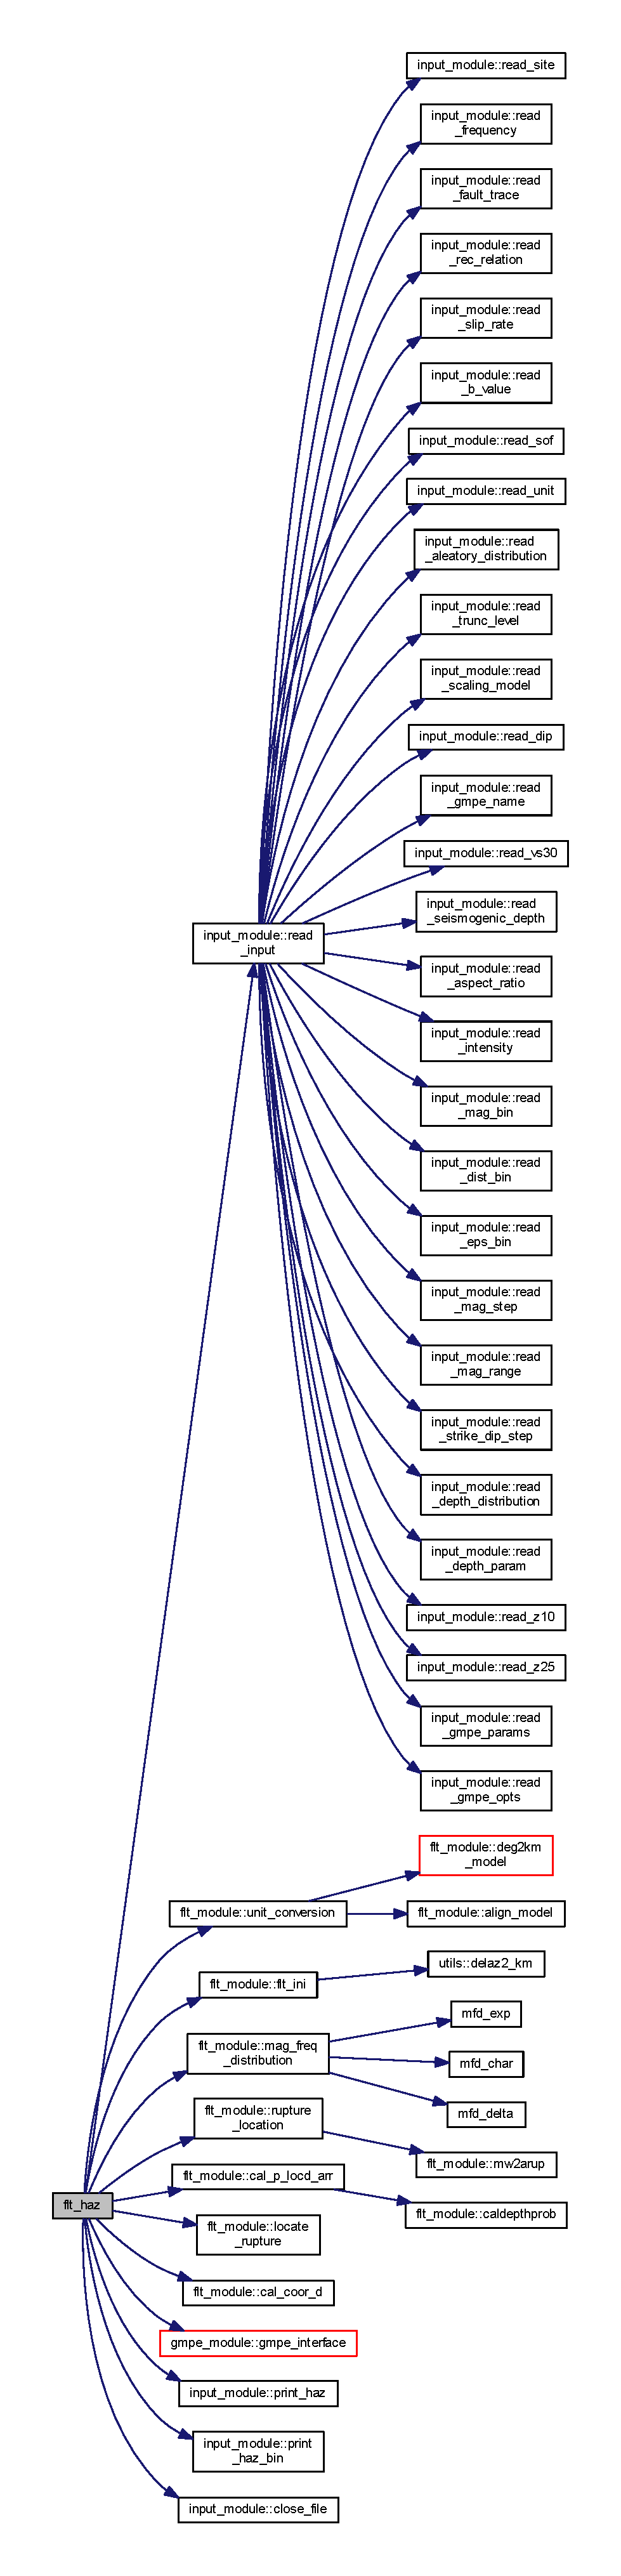
\includegraphics[height=550pt]{main__flt__haz_8f90_a7af4fe9056aa6bfbf0aca482e05e9503_cgraph}
\end{center}
\end{figure}



\hypertarget{utils_8f90}{}\section{utils.\+f90 File Reference}
\label{utils_8f90}\index{utils.\+f90@{utils.\+f90}}
\subsection*{Modules}
\begin{DoxyCompactItemize}
\item 
module \hyperlink{namespaceutils}{utils}
\end{DoxyCompactItemize}
\subsection*{Functions/\+Subroutines}
\begin{DoxyCompactItemize}
\item 
subroutine \hyperlink{namespaceutils_a6c61290deedf912e6810628145911f85}{utils\+::locate} (ibin, edge, x)
\item 
subroutine \hyperlink{namespaceutils_aa0f32919ddbbde1b5238425529660459}{utils\+::deg2km\+\_\+simple} (vn, ve, alat\+\_\+sta, alon\+\_\+sta,                                           alat\+\_\+ref, alon\+\_\+ref)
\item 
subroutine \hyperlink{namespaceutils_aa1dce66e1b3b67f4ff37fa7a949cb7b4}{utils\+::delaz2\+\_\+km} (y1, x1, y2, x2, delta, az)
\item 
elemental real(8) function \hyperlink{namespaceutils_aa41cc7594a2b7ecd3f3931859172f175}{utils\+::normcdf} (x)
\item 
elemental real(8) function \hyperlink{namespaceutils_a568d3767bca697c86b861637a25888f8}{utils\+::deltacdf} (x)
\item 
subroutine \hyperlink{namespaceutils_ac313e8810c0e461aa91b7299c8fba4be}{utils\+::truncnormcdf} (x, a, b, z)
\item 
double precision function \hyperlink{namespaceutils_a64e66c94f05898717cbc1863f70c9be1}{utils\+::m22det} (A)
\item 
double precision function \hyperlink{namespaceutils_a9bad87c0b79a45b5c6e6bbfcb2c6a126}{utils\+::m33det} (A)
\item 
subroutine \hyperlink{namespaceutils_aa037ebfaff3336105e73f563fdab02a8}{utils\+::pointlinesegdistance} (a, b, x, dist)
\item 
subroutine \hyperlink{namespaceutils_aebfee5643eb6828d1b6fd64229189af0}{utils\+::pointtriangledistance} (T\+R\+I1, T\+R\+I2, T\+R\+I3, P, dist)
\item 
real(8) function \hyperlink{namespaceutils_ab5a1a9ca34591c37c7fb606189317e16}{utils\+::dot3} (x, y)
\item 
subroutine \hyperlink{namespaceutils_af6906785e7d185fbdf7034969aababc4}{utils\+::dist\+\_\+rup\+\_\+seg} (Rrup, Rjb, Rx, coor, Ztor, strike, dip, rup\+\_\+wid)
\item 
real(8) function \hyperlink{namespaceutils_aa1727e2ba89368130186d248fd7b71b4}{utils\+::cal\+\_\+rx} (coor)
\item 
subroutine \hyperlink{namespaceutils_a3dfc1e25be8aa02534fda1a437ec9855}{utils\+::dist\+\_\+rup\+\_\+set} (Rrup, Rjb, Rx, coor, Ztor, strike, dip, rup\+\_\+wid)
\item 
subroutine \hyperlink{namespaceutils_ae3d121578601cfdb0b2687656ea19761}{utils\+::interp\+\_\+coeff} (x1, x2, y1, y2, x, y, iflag)
\item 
subroutine \hyperlink{namespaceutils_a47c34e02c3a6ca718ff160f085117f47}{utils\+::prob\+\_\+exceed} (p\+\_\+exceed, m\+\_\+eps, m\+\_\+aleatory\+\_\+distribution, trunclevel)
\end{DoxyCompactItemize}

%--- End generated contents ---

% Index
\backmatter
\newpage
\phantomsection
\clearemptydoublepage
\addcontentsline{toc}{chapter}{Index}
\printindex

\end{document}
